\documentclass[11pt,a4paper]{article}
\usepackage{fontspec}
\setmainfont{TeX Gyre Termes}
\setsansfont{TeX Gyre Heros}
\setmonofont[Scale=0.86]{DejaVu Sans Mono}
\usepackage[a4paper,left=2cm,right=2cm,top=2.2cm,bottom=2.2cm,headheight=28pt]{geometry}
\usepackage{graphicx,xcolor,tikz,amssymb,array,longtable,diagbox,enumitem,fancyhdr,titlesec}
\usepackage[most]{tcolorbox}
\usepackage{needspace}
\renewcommand{\contentsname}{Mục lục}
\usepackage[hidelinks]{hyperref}
\usepackage{bookmark}
\definecolor{brew}{HTML}{573520}
\definecolor{cream}{HTML}{F7F1EA}
\definecolor{amber}{HTML}{B4690E}
\definecolor{good}{HTML}{2F7D3A}
\definecolor{soft}{HTML}{6D5A49}
\setlength{\parindent}{0pt}
\setlength{\parskip}{3pt}
\sloppy\setlength{\emergencystretch}{3em}
\setlength{\fboxsep}{0pt}

\titleformat{\part}[display]{\sffamily\bfseries\Huge\color{brew}\centering}{\large PHẦN \thepart}{6pt}{}[\vspace{4pt}{\color{amber}\rule{0.3\textwidth}{1.2pt}}]
\titleformat{\section}{\sffamily\bfseries\Large\color{brew}}{\thesection.}{0.5em}{}
\titleformat{\subsection}{\sffamily\bfseries\large\color{brew}}{\thesubsection}{0.5em}{}
\renewcommand{\thepart}{\Roman{part}}
\pagestyle{fancy}\fancyhf{}
\lhead{\small\sffamily\color{soft} BrewLite -- Bộ câu hỏi vấn đáp và bài tập}
\rhead{\small\sffamily\color{soft} Lâm Sơn Hùng -- 3123560031}
\cfoot{\small\sffamily\thepage}
\renewcommand{\headrulewidth}{0.4pt}

% Mức độ câu hỏi
\newcommand{\dotlv}[1]{\textcolor{amber}{#1}}
\newcommand{\lvA}{\dotlv{$\bullet$}\textcolor{black!20}{$\bullet\bullet$}}
\newcommand{\lvB}{\dotlv{$\bullet\bullet$}\textcolor{black!20}{$\bullet$}}
\newcommand{\lvC}{\dotlv{$\bullet\bullet\bullet$}}
\newcommand{\chk}{\raisebox{-1pt}{\tikz\draw[soft,line width=0.6pt] (0,0) rectangle (9pt,9pt);}}

% Câu hỏi + gợi ý
\newcommand{\qa}[4]{%
  \par\needspace{5\baselineskip}\vspace{5pt}\noindent
  {\sffamily\bfseries\color{brew}Câu #1.}\ {\bfseries #3}\hfill{\small #2}\,\chk\par\nopagebreak[4]\vspace{1pt}
  \begin{tcolorbox}[enhanced,breakable,colback=cream,colframe=cream,boxrule=0pt,left=6pt,right=6pt,top=3pt,bottom=3pt,arc=2pt,
    borderline west={2pt}{0pt}{amber},before skip=0pt,after skip=2pt]
  {\small\sffamily\color{soft}Gợi ý trả lời.}\ {\small #4}
  \end{tcolorbox}}

% Bài tập
\newcommand{\exq}[2]{\par\needspace{6\baselineskip}\vspace{8pt}\noindent{\sffamily\bfseries\color{brew}Bài #1.}\ #2\par\nopagebreak[4]}
\newcommand{\writelines}[1]{\vspace{2pt}\foreach \i in {1,...,#1}{\par\noindent\textcolor{black!35}{\dotfill}\par\vspace{5pt}}}
\newcommand{\drawgrid}[1]{\par\nopagebreak[4]\vspace{3pt}\noindent\begin{tikzpicture}
  \draw[step=0.5cm,black!12,very thin] (0,0) grid (\linewidth,#1);
  \draw[black!40] (0,0) rectangle (\linewidth,#1);
  \node[anchor=north west,font=\scriptsize\sffamily,text=black!45] at (0.1,#1) {Vẽ vào đây};
\end{tikzpicture}\par}
\newcommand{\ansq}[2]{\par\vspace{3pt}\noindent\hangindent=1.1cm\hangafter=1\makebox[1.1cm][l]{\sffamily\bfseries\color{good}#1}{\small #2}\par}

\begin{document}

% ---------------- Bìa ----------------
\begin{titlepage}
\centering
{\sffamily\small TRƯỜNG ĐẠI HỌC SÀI GÒN\\ KHOA CÔNG NGHỆ THÔNG TIN}\\[1cm]

\includegraphics[width=2.6cm]{img/logo.png}\\[1.2cm]
{\sffamily\large\color{soft} Môn Công nghệ Phần mềm -- Bài tập lớn BrewLite}\\[0.6cm]
{\sffamily\bfseries\Huge\color{brew} Bộ câu hỏi vấn đáp}\\[0.25cm]
{\sffamily\bfseries\Huge\color{brew} và bài tập ôn luyện}\\[0.5cm]
{\color{amber}\rule{0.35\textwidth}{1.5pt}}\\[0.5cm]
{\large Lý thuyết nền tảng $\cdot$ Luồng hoạt động $\cdot$ Toàn bộ sơ đồ $\cdot$ Kiến trúc $\cdot$ Kiểm thử $\cdot$ CI/CD $\cdot$ Demo}\\[0.3cm]
{\large Assignment 1 và Assignment 2}\\[1.6cm]
\begin{tabular}{rl}
Sinh viên: & Lâm Sơn Hùng -- 3123560031\\
Giảng viên: & Từ Lãng Phiêu\\
Nội dung: & 183 câu hỏi có gợi ý trả lời, 43 bài tập có đáp án
\end{tabular}
\vfill
{\small TP. Hồ Chí Minh, tháng 11/2026}
\end{titlepage}

% ---------------- Cách dùng ----------------
\section*{Cách dùng tài liệu}
\begin{itemize}[leftmargin=1.2em,itemsep=2pt]
  \item \textbf{Phần I} gồm các câu thầy có thể hỏi, chia theo chủ đề. Mỗi câu có \textbf{gợi ý trả lời} viết sát với đồ án (đúng tên file, số liệu, mã lỗi). Hãy tự trả lời thành tiếng trước, rồi mới đọc gợi ý.
  \item Mức độ: \lvA\ cơ bản (chắc chắn bị hỏi), \lvB\ hiểu sâu, \lvC\ nâng cao hoặc câu bẫy. Trả lời được thì đánh dấu vào ô \chk.
  \item Đầu mỗi chương sơ đồ có hình thật của đồ án để vừa nhìn vừa giải thích, như khi thầy chỉ vào sơ đồ trong báo cáo.
  \item Chương \textbf{Demo giao diện và chức năng} là các yêu cầu thao tác trực tiếp; gợi ý cho biết phải bấm gì và chỉ ra kết quả nào trên màn hình.
  \item \textbf{Phần II} là bài tập để làm ngay trong tài liệu (dòng trống và khung vẽ). \textbf{Phần III} là đáp án.
\end{itemize}

\subsection*{Những con số và tên cần thuộc}
\renewcommand{\arraystretch}{1.25}
\begin{longtable}{|p{4.2cm}|p{11.8cm}|}
\hline
Scrum A1 & 3 Sprint $\times$ 10 ngày, 10 task, 33 SP (10 + 9 + 14); Task 10 = 8 SP \\ \hline
Scrum A2 & 5 task tuần tự, 2 Sprint: Sprint 1 = 27 SP, Sprint 2 = 32 SP \\ \hline
Yêu cầu & FR-01..FR-15, NFR-01..NFR-11; UC-05 Đặt và thanh toán (A1..A5, E1..E8); US-01..US-14 \\ \hline
Use case & A1: 13 use case; A2: UC-01..UC-12; 3 actor: Khách hàng, Nhân viên, Cổng thanh toán \\ \hline
DFD & Mức 0: 1 tiến trình, 3 tác nhân; mức 1: 6 tiến trình, 5 kho D1..D5 \\ \hline
State machine & 7 trạng thái, 9 chuyển tiếp hợp lệ / 49 cặp; sai trả 409 INVALID\_TRANSITION \\ \hline
CSDL & users, products, orders, order\_items, payments, promotions, loyalty\_transactions; 2 migration \\ \hline
Giá & Size S $-$5.000, M 0, L +7.000; topping 5.000 / 7.000 / 5.000 / 10.000 \\ \hline
Khuyến mãi, điểm & BREW10 10\% tối đa 20.000; WELCOME20 20\% đơn từ 100.000 tối đa 50.000; 1 điểm / 10.000đ \\ \hline
HTTP & 201 tạo, 200 phát lại, 400 sai dữ liệu, 401 chưa đăng nhập, 402 thanh toán lỗi, 403 không quyền, 404, 409 xung đột \\ \hline
Đồng thời & Optimistic lock cột version, thử lại $\le$ 8; thanh toán khóa dòng FOR UPDATE; UNIQUE idempotencyKey \\ \hline
Kiểm thử & 15 unit + 27 integration + 7 component + 1 E2E = 50 (A2); 55 kịch bản, 224 điểm kiểm tra, 6 lỗi (A1) \\ \hline
Cổng & web 3000, API 3001, PostgreSQL 5432; health: GET /health \\ \hline
CI & Install $\rightarrow$ Lint $\rightarrow$ Unit Test $\rightarrow$ Build (+ integration, E2E, gitleaks) \\ \hline
CD & Push/Tag $\rightarrow$ Lint và Test $\rightarrow$ Build $\rightarrow$ Docker Image (SHA) $\rightarrow$ GHCR $\rightarrow$ Deploy Render $\rightarrow$ Smoke Test $\rightarrow$ (lỗi) Rollback \\ \hline
Kiến trúc & C4 mức 1–2, 3 lớp, 7 ADR, modular monolith; Render Singapore, DB không public \\ \hline
Tài khoản demo & staff@brewlite.local / staff123 (local); khách tự đăng ký \\ \hline
\end{longtable}

\newpage
\tableofcontents
\newpage

\part{Câu hỏi vấn đáp và gợi ý trả lời}
\section{Agile, Scrum và quy trình làm việc}
\noindent\textit{Lý thuyết Scrum và cách đồ án áp dụng ở Assignment 1 (3 Sprint, 10 task) và Assignment 2 (2 Sprint, 5 task).} \hfill \small(15 câu)\normalsize\par\medskip
\begin{center}
\fbox{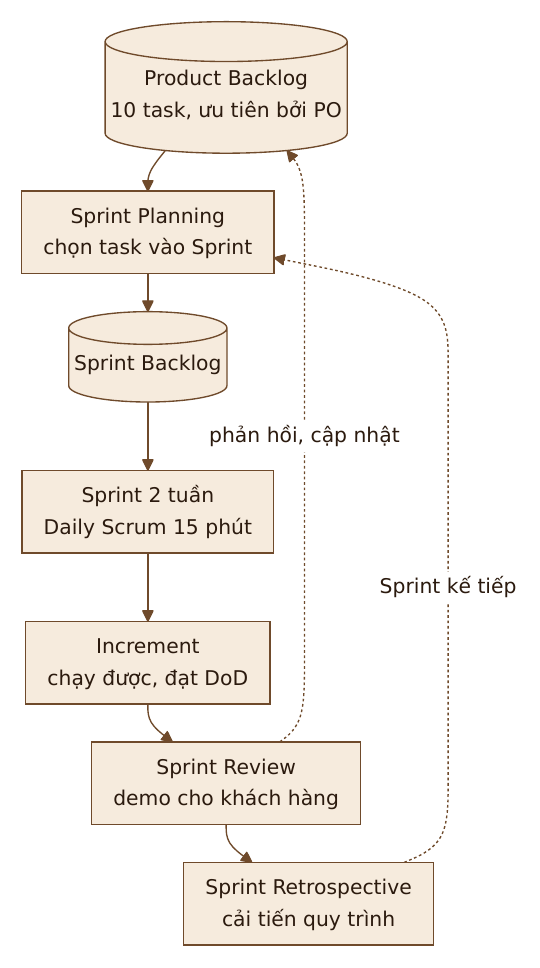
\includegraphics[width=0.62\textwidth,height=0.30\textheight,keepaspectratio]{img/a1/scrum.png}}\hspace{2mm}
\end{center}\vspace{-2mm}
\qa{1}{\lvA}{Agile là gì? Tuyên ngôn Agile gồm những giá trị nào?}{Agile là cách phát triển theo vòng lặp ngắn, giao phần mềm chạy được sớm, nhận phản hồi rồi điều chỉnh. 4 giá trị: con người và tương tác hơn quy trình và công cụ; phần mềm chạy được hơn tài liệu đầy đủ; hợp tác với khách hàng hơn đàm phán hợp đồng; phản hồi thay đổi hơn bám theo kế hoạch. Vế phải vẫn có giá trị, chỉ là vế trái được ưu tiên hơn.}
\qa{2}{\lvA}{Scrum có những vai trò, sự kiện và tạo phẩm nào?}{3 vai trò: Product Owner, Scrum Master, Development Team. 5 sự kiện: Sprint, Sprint Planning, Daily Scrum (15 phút), Sprint Review, Sprint Retrospective. 3 tạo phẩm: Product Backlog, Sprint Backlog, Increment.}
\qa{3}{\lvA}{Product Owner và Scrum Master khác nhau thế nào?}{PO quyết định làm gì và thứ tự ưu tiên (quản lý Product Backlog, nghiệm thu). SM bảo vệ quy trình: điều phối sự kiện, gỡ vướng mắc, giúp nhóm áp dụng Scrum đúng. PO trả lời 'làm cái gì', SM giúp 'làm thế nào cho đúng quy trình'.}
\qa{4}{\lvA}{Sprint Review khác Sprint Retrospective ra sao?}{Review nhìn vào SẢN PHẨM: demo Increment cho PO/khách hàng, nhận phản hồi, cập nhật backlog. Retrospective nhìn vào QUY TRÌNH: nhóm tự hỏi điều gì làm tốt, điều gì cần cải thiện và chọn hành động cho Sprint sau.}
\qa{5}{\lvB}{Em làm một mình thì áp dụng Scrum thế nào?}{Em kiêm cả PO, SM và Developer. Vẫn giữ đủ sự kiện ở quy mô cá nhân: lập kế hoạch đầu Sprint, cập nhật tiến độ hằng ngày (burndown), demo cuối Sprint, viết retrospective. Backlog có ưu tiên và story point; Definition of Done dùng để quyết định task đã xong chưa.}
\qa{6}{\lvA}{Story point là gì? Vì sao không ước lượng bằng giờ?}{Story point đo độ lớn tương đối (độ phức tạp, khối lượng, rủi ro) của một hạng mục, thường dùng dãy Fibonacci. Ước lượng tương đối nhanh và ổn định hơn ước lượng giờ, vì con người so sánh 'cái này to gấp đôi cái kia' tốt hơn đoán chính xác thời gian.}
\qa{7}{\lvA}{Velocity và burndown chart dùng để làm gì?}{Velocity là số story point hoàn thành mỗi Sprint, dùng để dự báo Sprint sau nhận được bao nhiêu việc. Burndown chart vẽ story point còn lại theo ngày; so đường thực tế với đường lý tưởng để biết đang chậm hay nhanh.}
\qa{8}{\lvB}{Definition of Done của đồ án gồm những gì?}{A1: code chạy không lỗi build, có commit rõ ràng, API validate và UI xử lý loading/lỗi, có README. A2 mở rộng thành 8 điểm: merge qua PR theo mẫu; CI xanh (lint, unit, build, integration, e2e, quét secret); có test cho hành vi mới; validate backend + loading/rỗng/lỗi frontend; đổi schema có migration kèm down(); tài liệu cập nhật cùng PR; không lộ secret; CD triển khai và smoke test đạt.}
\qa{9}{\lvB}{Definition of Done khác Acceptance Criteria thế nào?}{Acceptance Criteria gắn với TỪNG user story (story này cần đạt điều kiện gì). Definition of Done áp dụng CHUNG cho mọi hạng mục (chất lượng tối thiểu: test, review, tài liệu, triển khai). Một story chỉ Done khi đạt cả hai.}
\qa{10}{\lvA}{Assignment 1 chia Sprint thế nào?}{3 Sprint, mỗi Sprint 10 ngày, 10 task, tổng 33 SP. Sprint 1: Task 1–4 (khởi tạo, API sản phẩm, menu, chi tiết) = 10 SP. Sprint 2: Task 5–7 (giỏ, API đơn, JWT) = 9 SP. Sprint 3: Task 8–10 (thanh toán, xác nhận/lịch sử/Docker, nghiệp vụ backend) = 14 SP vì Task 10 chiếm 8 SP.}
\qa{11}{\lvA}{Assignment 2 chia Sprint thế nào?}{2 Sprint. Sprint 1 (27 SP, 11 hạng mục): tài liệu Task 1–3, repo, quy ước, CI, MVP xem menu. Sprint 2 (32 SP, 13 hạng mục): hoàn thiện MVP, migration, health, PWA, E2E, CD, triển khai production, bàn giao.}
\qa{12}{\lvA}{Sprint Goal là gì? Cho ví dụ trong đồ án.}{Một câu nêu mục tiêu của Sprint, giúp nhóm ra quyết định khi phát sinh. Sprint 1 A2: 'Tạo nền tảng kỹ thuật, tài liệu có kiểm soát phiên bản và MVP đầu tiên chạy được cho luồng xem menu'. Sprint 2 A2: 'Hoàn thành luồng end-to-end, tự động hóa đóng gói và triển khai một phiên bản production'.}
\qa{13}{\lvB}{Vì sao đề A2 yêu cầu làm 5 task tuần tự?}{Để mô phỏng đúng vòng đời: yêu cầu phải có trước mới mô hình hóa, mô hình có trước mới thiết kế kiến trúc, rồi mới code. Task sau chỉ được nghiệm thu khi tạo phẩm task trước đã có trên repo với lịch sử rõ ràng; vì vậy git của em có các commit docs(task1) $\rightarrow$ docs(task2) $\rightarrow$ docs(task3) $\rightarrow$ chore(task4) $\rightarrow$ feat(task5).}
\qa{14}{\lvA}{MVP là gì? MVP khác prototype/mockup thế nào?}{MVP (Minimum Viable Product) là phiên bản nhỏ nhất CHẠY ĐƯỢC, đủ tính năng cốt lõi để kiểm chứng giả thuyết với người dùng thật. Mockup chỉ là hình tĩnh; prototype có thể bấm thử nhưng thường không có backend thật.}
\qa{15}{\lvC}{Nếu PO đổi yêu cầu giữa Sprint thì em xử lý thế nào?}{Không đưa thẳng vào Sprint đang chạy nếu làm lệch Sprint Goal: ghi vào Product Backlog, PO ưu tiên lại, đưa vào Sprint sau. Nếu thay đổi khẩn cấp làm Sprint Goal mất ý nghĩa thì PO có thể hủy Sprint và lập kế hoạch lại. Tài liệu yêu cầu đổi qua pull request có ghi lý do.}
\section{Khai thác và đặc tả yêu cầu}
\noindent\textit{Stakeholder, phạm vi, FR/NFR, user story, tiêu chí chấp nhận, MoSCoW, đặc tả UC-05 (Task 1 của A2).} \hfill \small(18 câu)\normalsize\par\medskip
\qa{16}{\lvA}{Product Vision của BrewLite là gì?}{'BrewLite giúp khách hàng đặt và thanh toán đồ uống không dùng tiền mặt chỉ trong vài chạm, giảm thời gian xếp hàng và nhận đơn nhanh tại quầy.'}
\qa{17}{\lvA}{Vấn đề nghiệp vụ mà BrewLite giải quyết?}{Giờ cao điểm hàng dài trước quầy, khách mất 1–3 phút gọi món và trả tiền nên bỏ về; nhân viên vừa nhận order vừa thu tiền dễ nhầm món/size/topping; quán không có dữ liệu đơn và chương trình khách hàng thân thiết.}
\qa{18}{\lvA}{Stakeholder là gì? Kể các stakeholder của đồ án.}{Stakeholder là người hoặc tổ chức bị ảnh hưởng hoặc có ảnh hưởng tới hệ thống. 6 nhóm: khách hàng, nhân viên quầy, quản lý cửa hàng, giảng viên/khách hàng nghiệm thu, nhóm phát triển, đơn vị thanh toán. Mỗi nhóm có mục tiêu và kỳ vọng riêng (ví dụ khách muốn không bị trừ tiền hai lần, quản lý muốn không bán vượt kho).}
\qa{19}{\lvA}{Phạm vi in-scope, mở rộng và out-of-scope khác nhau thế nào?}{In-scope: làm trong MVP (FR-01..FR-13, health, CI/CD). Mở rộng: chưa làm bản này nhưng có trong backlog (giao diện nhân viên, cổng thật, thông báo READY, đơn tự hết hạn). Out-of-scope: không làm trong dự án (giao hàng, tiền mặt, nhiều chi nhánh, app native, kế toán, lưu thẻ).}
\qa{20}{\lvB}{Giả định và ràng buộc khác nhau ra sao? Cho ví dụ.}{Giả định là điều coi là đúng nhưng chưa kiểm chứng, nếu sai thì phải xem lại thiết kế (A-01 khách có smartphone và Internet; A-03 cổng mô phỏng hành xử như cổng thật). Ràng buộc là điều bắt buộc phải tuân theo (C-01 bắt buộc Next.js, NestJS, PostgreSQL; C-03 ngân sách 0 đồng; C-05 secret không vào repo).}
\qa{21}{\lvB}{Kể các rủi ro ban đầu và biện pháp.}{R-01 trừ tiền hai lần $\rightarrow$ Idempotency-Key, UNIQUE, khóa dòng. R-02 bán vượt kho $\rightarrow$ optimistic lock, CHECK stock \textgreater{}= 0. R-03 một người làm dễ trễ $\rightarrow$ MoSCoW, tự động hóa. R-04 gói miễn phí Render ngủ/Postgres hết hạn $\rightarrow$ smoke test thử lại, mở URL trước giờ chấm. R-05 lộ secret $\rightarrow$ .gitignore, gitleaks. R-06 migration lỗi $\rightarrow$ 1 transaction, health check. R-07 lệch giá $\rightarrow$ server tính lại, hỏi khách.}
\qa{22}{\lvA}{Yêu cầu chức năng và phi chức năng khác nhau thế nào?}{FR mô tả hệ thống LÀM GÌ (xem menu, đặt đơn, thanh toán). NFR mô tả hệ thống làm TỐT ĐẾN ĐÂU (hiệu năng \textless{} 500 ms, bảo mật bcrypt/JWT, khả dụng trên di động, khả năng triển khai).}
\qa{23}{\lvA}{SRS của em có bao nhiêu FR, NFR? Kể vài cái.}{FR-01..FR-15 và NFR-01..NFR-11. Ví dụ FR-01 xem menu, FR-05 đặt đơn, FR-07 thanh toán idempotent, FR-10 state machine, FR-12 điểm thưởng, FR-13 PWA; NFR-01 p95 \textless{} 500 ms, NFR-03 bảo mật xác thực, NFR-04 toàn vẹn giao dịch, NFR-07 tính sẵn sàng, NFR-08 khả năng triển khai.}
\qa{24}{\lvA}{MoSCoW là gì? Em xếp yêu cầu ra sao?}{Must / Should / Could / Won't (this time). Must: luồng menu $\rightarrow$ giỏ $\rightarrow$ đăng nhập $\rightarrow$ đặt đơn $\rightarrow$ thanh toán $\rightarrow$ xác nhận, state machine, NFR bảo mật và triển khai. Should: mã giảm giá, hủy đơn, điểm thưởng. Could: PWA. Won't (bản 2.0): giao diện nhân viên, thông báo đơn READY.}
\qa{25}{\lvB}{Tiêu chí chấp nhận tốt phải như thế nào?}{Kiểm chứng được bằng đúng/sai, có điều kiện và kết quả cụ thể, viết được thành test. Ví dụ tốt: 'POST /payments thiếu Idempotency-Key trả 400'. Ví dụ kém: 'thanh toán phải an toàn'. Có thể viết dạng Given/When/Then.}
\qa{26}{\lvA}{User story có cấu trúc thế nào? Cho ví dụ của đồ án.}{'Là \textless{}vai trò\textgreater{}, tôi muốn \textless{}mục tiêu\textgreater{} để \textless{}lợi ích\textgreater{}.' Ví dụ US-07: 'Là khách hàng, tôi muốn bấm thanh toán nhiều lần hoặc mất mạng mà không bị trừ tiền hai lần.' Tiêu chí: cùng Idempotency-Key chỉ tạo 1 đơn/1 giao dịch. A1 có US-01..US-09; A2 bổ sung US-10..US-14.}
\qa{27}{\lvB}{Tiêu chí INVEST của user story?}{Independent (độc lập), Negotiable (thương lượng được), Valuable (có giá trị), Estimable (ước lượng được), Small (đủ nhỏ để làm trong một Sprint), Testable (kiểm thử được).}
\qa{28}{\lvA}{Use-case trọng tâm em chọn là gì và vì sao?}{UC-05 Đặt và thanh toán đơn hàng, vì tạo ra doanh thu và chứa các rủi ro lớn nhất: trừ tiền hai lần, bán vượt kho, thanh toán lỗi.}
\qa{29}{\lvA}{Đặc tả UC-05 gồm những mục nào?}{Mã/tên, actor chính (Khách hàng) và phụ (Cổng thanh toán), trigger (bấm Thanh toán ở /cart), yêu cầu liên quan, include/extend, tiền điều kiện (giỏ $\ge$ 1 món), hậu điều kiện thành công và thất bại, luồng chính 10 bước, luồng thay thế A1..A5, luồng ngoại lệ E1..E8, quy tắc đặc biệt, bảng tiêu chí $\rightarrow$ test.}
\qa{30}{\lvB}{Luồng thay thế khác luồng ngoại lệ thế nào? Kể các luồng của UC-05.}{Thay thế (A): vẫn đạt mục tiêu theo đường khác. Ngoại lệ (E): không đạt, hệ thống xử lý lỗi có kiểm soát. A1 chưa đăng nhập; A2 nhập mã hợp lệ; A3 giá server khác giỏ; A4 gửi lặp cùng key; A5 thanh toán lại đơn PAYMENT\_FAILED. E1 dữ liệu sai 400; E2 mã giảm giá sai; E3 hết hàng 409; E4 token hết hạn 401; E5 cổng từ chối 402; E6 đơn không thanh toán được 409; E7 key dùng cho đơn khác 409; E8 mất kết nối.}
\qa{31}{\lvB}{Hậu điều kiện thành công của UC-05?}{Đúng 1 đơn PAID với giá server tính; đúng 1 payment SUCCESS gắn Idempotency-Key; tồn kho giảm đúng số ly; khách được cộng $\lfloor$tổng/10.000$\rfloor$ điểm và có 1 LoyaltyTransaction EARN; giỏ được xóa; khách thấy trang /orders/:id.}
\qa{32}{\lvB}{Quy tắc nghiệp vụ BR-01..BR-05 là gì?}{BR-01 đơn giá = giá gốc size M + chênh lệch size + tổng topping khác nhau. BR-02 giảm = $\lfloor$tạm tính $\times$ \% / 100$\rfloor$, không vượt trần. BR-03 điểm = $\lfloor$tổng / 10.000$\rfloor$, cộng một lần khi PAID, thu hồi khi hủy. BR-04 giữ kho khi tạo đơn, trả kho khi hủy. BR-05 chỉ đơn PENDING/PAYMENT\_FAILED được thanh toán.}
\qa{33}{\lvC}{Làm sao chứng minh tiêu chí chấp nhận đã được dùng để viết test?}{Mỗi dòng SRS có cột Test với mã cụ thể (ví dụ FR-07 $\rightarrow$ INT-T08, T09, T10, T16, T17), và ma trận truy vết nối yêu cầu $\rightarrow$ use-case $\rightarrow$ sơ đồ $\rightarrow$ code $\rightarrow$ test. Tên test trong code bắt đầu bằng đúng mã đó.}
\section{Sơ đồ Use Case}
\noindent\textit{Use case tổng quát A1 (13 use case) và A2 (UC-01..UC-12), use case UC-05.} \hfill \small(9 câu)\normalsize\par\medskip
\begin{center}
\fbox{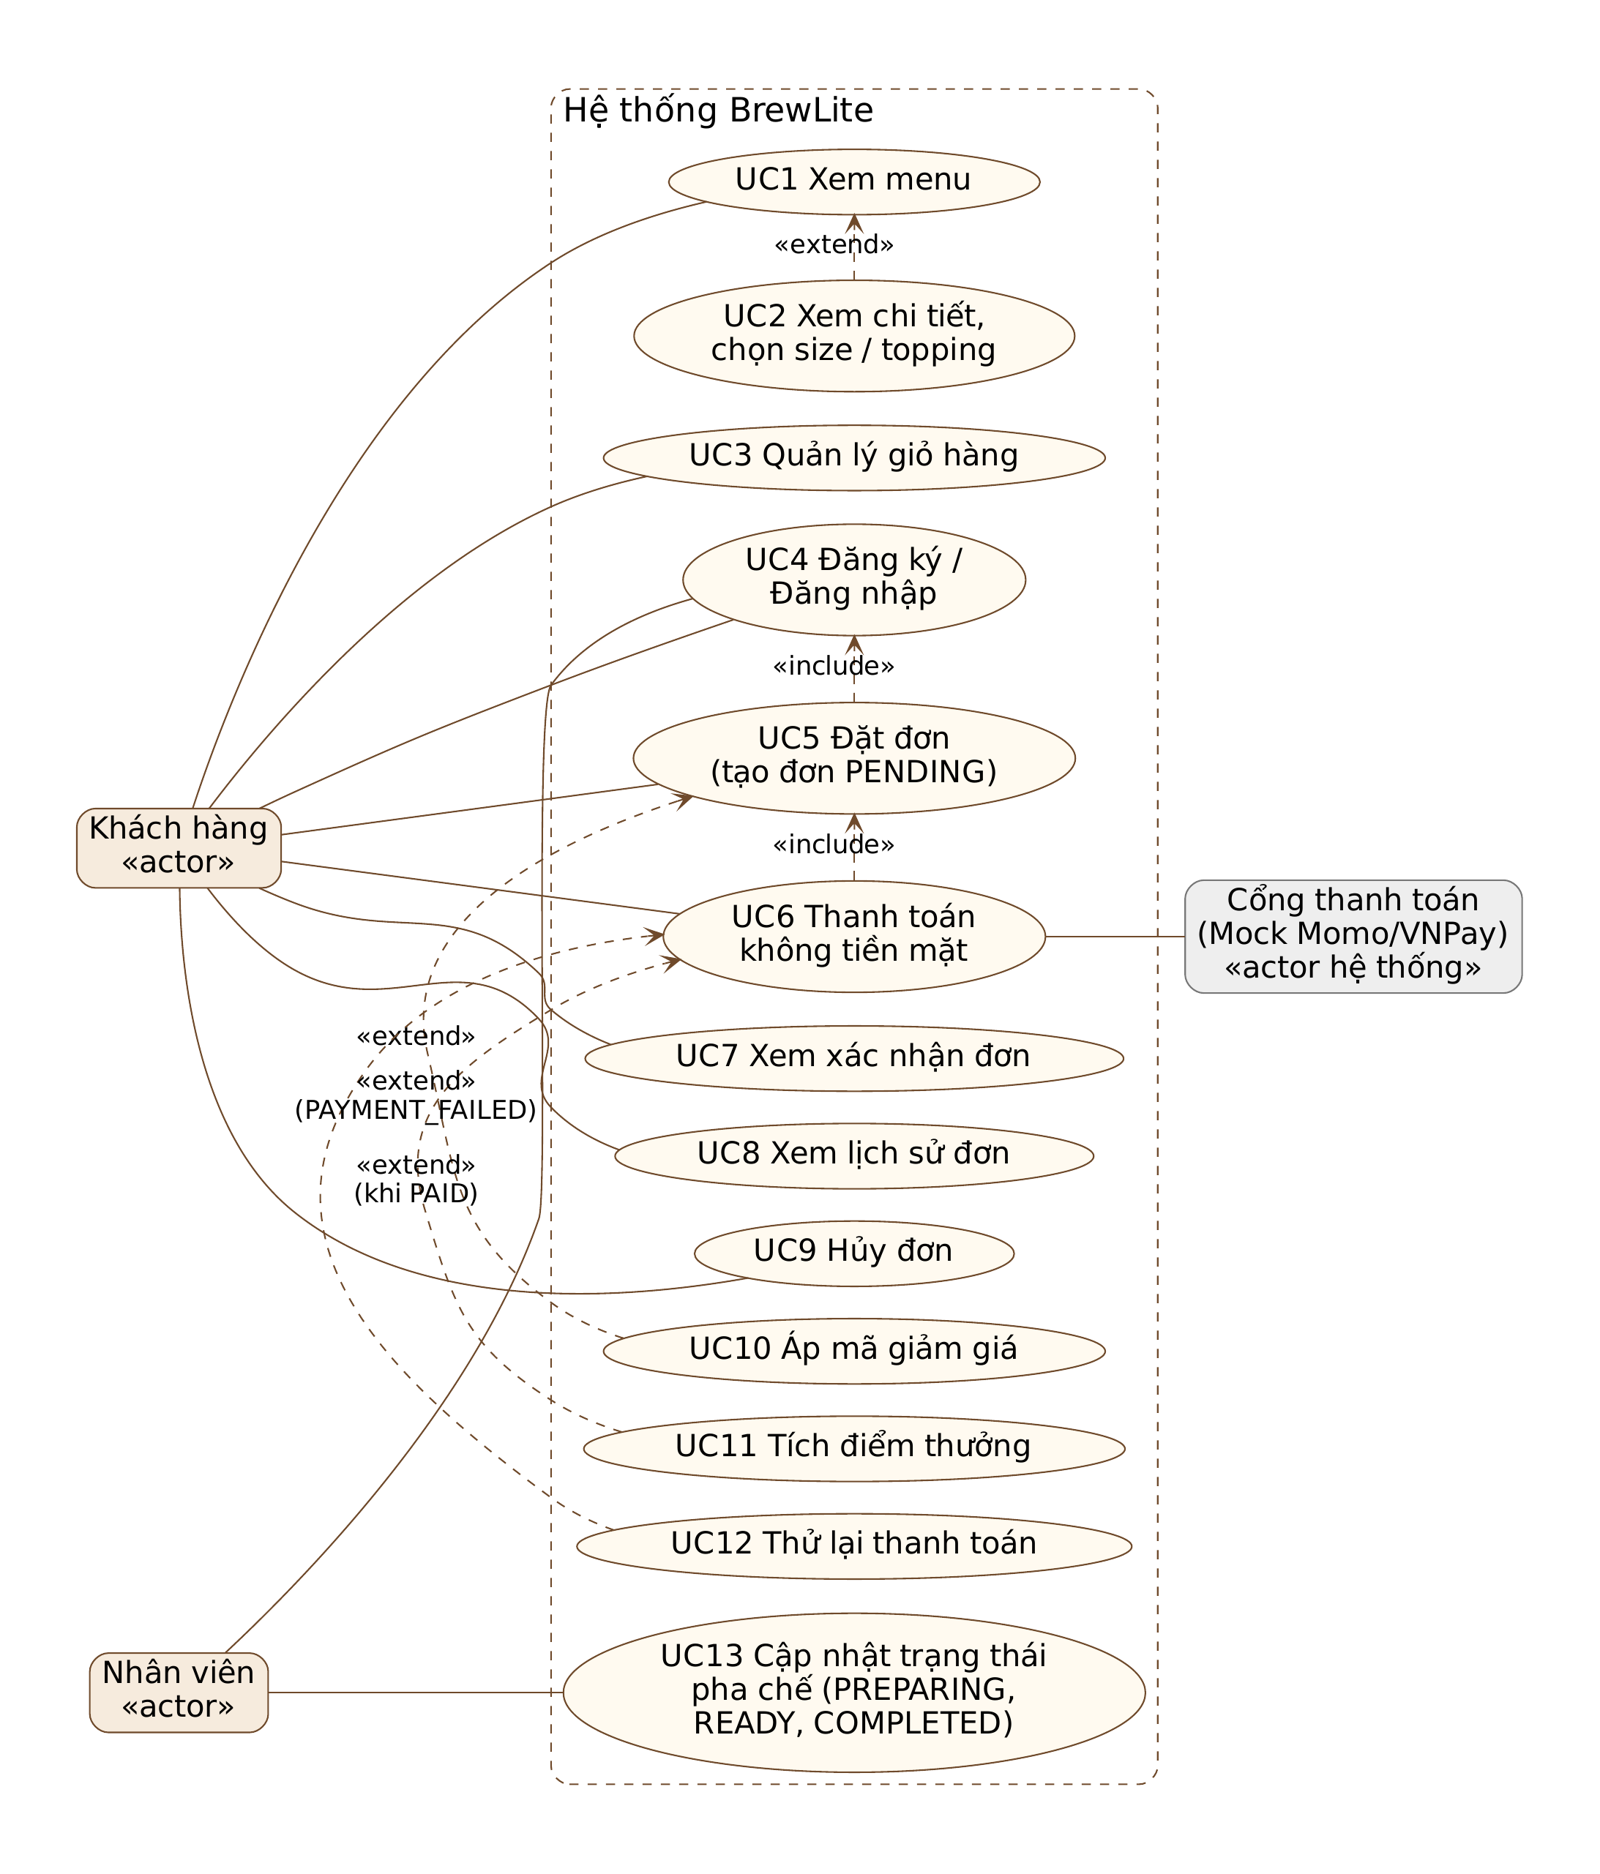
\includegraphics[width=0.47\textwidth,height=0.30\textheight,keepaspectratio]{img/a1/usecase.png}}\hspace{2mm}
\fbox{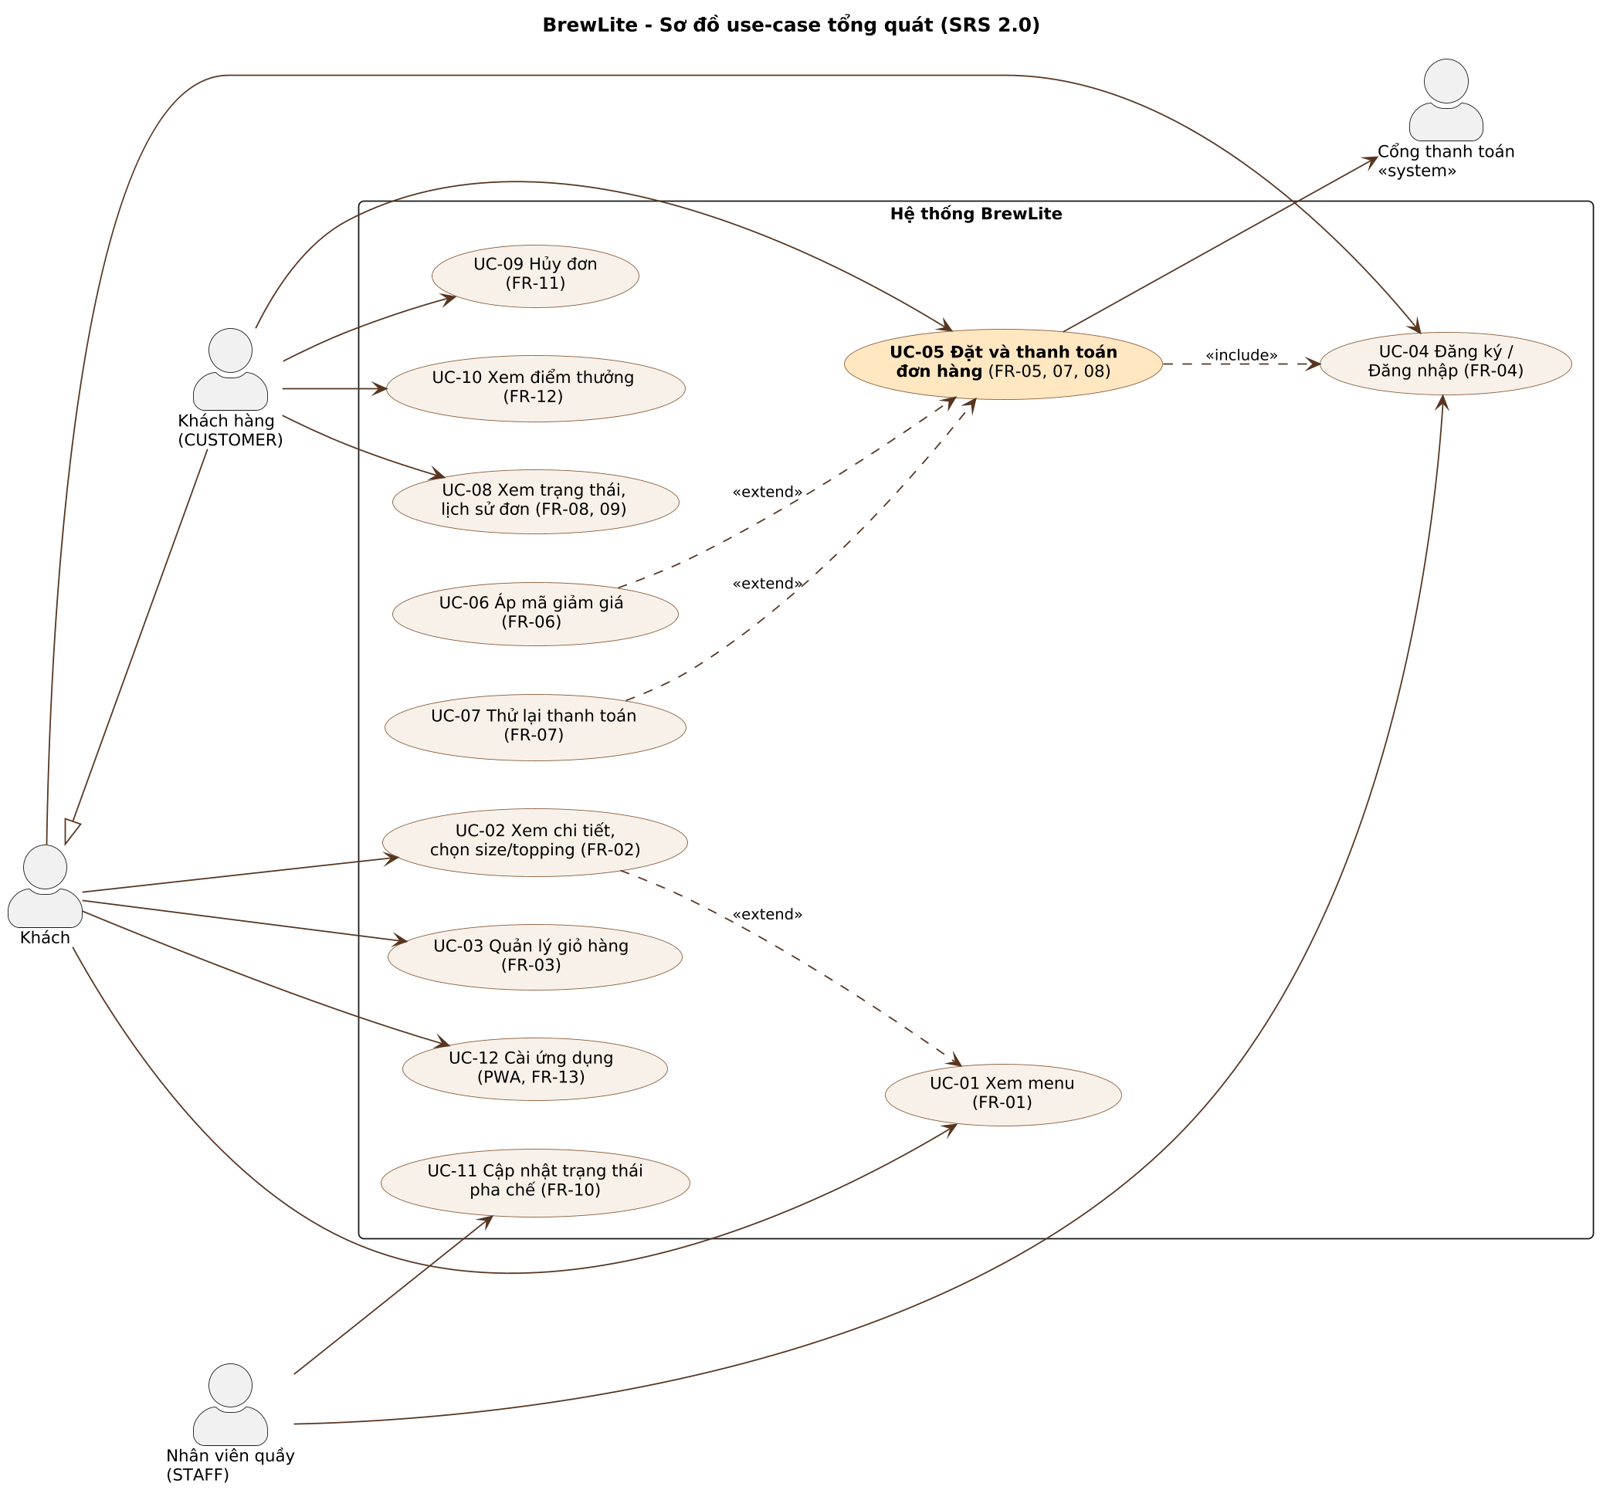
\includegraphics[width=0.47\textwidth,height=0.30\textheight,keepaspectratio]{img/a2/usecase-overview.png}}\hspace{2mm}
\end{center}\vspace{-2mm}
\qa{34}{\lvA}{Sơ đồ use case dùng để làm gì?}{Mô tả hệ thống từ góc nhìn bên ngoài: AI (actor) dùng hệ thống để LÀM GÌ (use case). Không mô tả cách làm bên trong hay thứ tự thời gian.}
\qa{35}{\lvA}{Các thành phần của sơ đồ use case?}{Actor (người que hoặc «actor»), use case (hình elip, tên động từ + danh từ), system boundary (hình chữ nhật), association (đường nối actor – use case), include, extend, generalization.}
\qa{36}{\lvA}{Include và extend khác nhau thế nào? Mũi tên chỉ hướng nào?}{Include: hành vi BẮT BUỘC, use case gốc luôn gọi use case được include; mũi tên đứt từ gốc tới use case được include. Extend: hành vi TÙY CHỌN, chỉ xảy ra khi có điều kiện; mũi tên đứt từ use case mở rộng về use case gốc.}
\qa{37}{\lvA}{Actor của BrewLite là ai?}{Khách hàng (A2 tách Khách chưa đăng nhập và Khách hàng CUSTOMER, có generalization), Nhân viên quầy (STAFF), Cổng thanh toán (actor hệ thống, mô phỏng).}
\qa{38}{\lvB}{Cổng thanh toán có phải actor không? Vì sao?}{Có. Actor là bất kỳ thực thể BÊN NGOÀI ranh giới hệ thống tương tác với hệ thống, có thể là người hoặc hệ thống khác. Cổng thanh toán là hệ thống ngoài nên vẽ là actor «system».}
\qa{39}{\lvB}{Trong sơ đồ của em, quan hệ nào là include, quan hệ nào là extend?}{A1: UC5 Đặt đơn include UC4 Đăng nhập; UC6 Thanh toán include UC5; UC2 extend UC1; UC10 Áp mã extend UC5; UC11 Tích điểm extend UC6 (khi PAID); UC12 Thử lại thanh toán extend UC6 (khi PAYMENT\_FAILED). A2: UC-05 include UC-04; UC-06 Áp mã extend UC-05; UC-07 Thử lại extend UC-05; UC-02 extend UC-01.}
\qa{40}{\lvA}{A1 có bao nhiêu use case? A2 có bao nhiêu?}{A1: 13 use case (UC1..UC13). A2 (SRS 2.0): 12 use case UC-01..UC-12, thêm UC-10 Xem điểm thưởng và UC-12 Cài ứng dụng PWA.}
\qa{41}{\lvB}{Generalization giữa Khách và Khách hàng nghĩa là gì?}{Khách hàng (đã đăng nhập) kế thừa mọi use case của Khách (xem menu, chi tiết, giỏ, đăng nhập) và có thêm use case riêng (đặt đơn, xem lịch sử, hủy đơn, xem điểm).}
\qa{42}{\lvB}{Lỗi thường gặp khi vẽ use case?}{Đặt tên use case là danh từ hoặc tên màn hình; vẽ use case quá nhỏ như 'bấm nút'; dùng use case để vẽ thứ tự bước (đó là việc của activity); nhầm hướng mũi tên include/extend; nối actor với nhau; để actor bên trong ranh giới hệ thống.}
\section{Sơ đồ dòng dữ liệu (DFD)}
\noindent\textit{DFD mức 0 và mức 1 của A1.} \hfill \small(8 câu)\normalsize\par\medskip
\begin{center}
\fbox{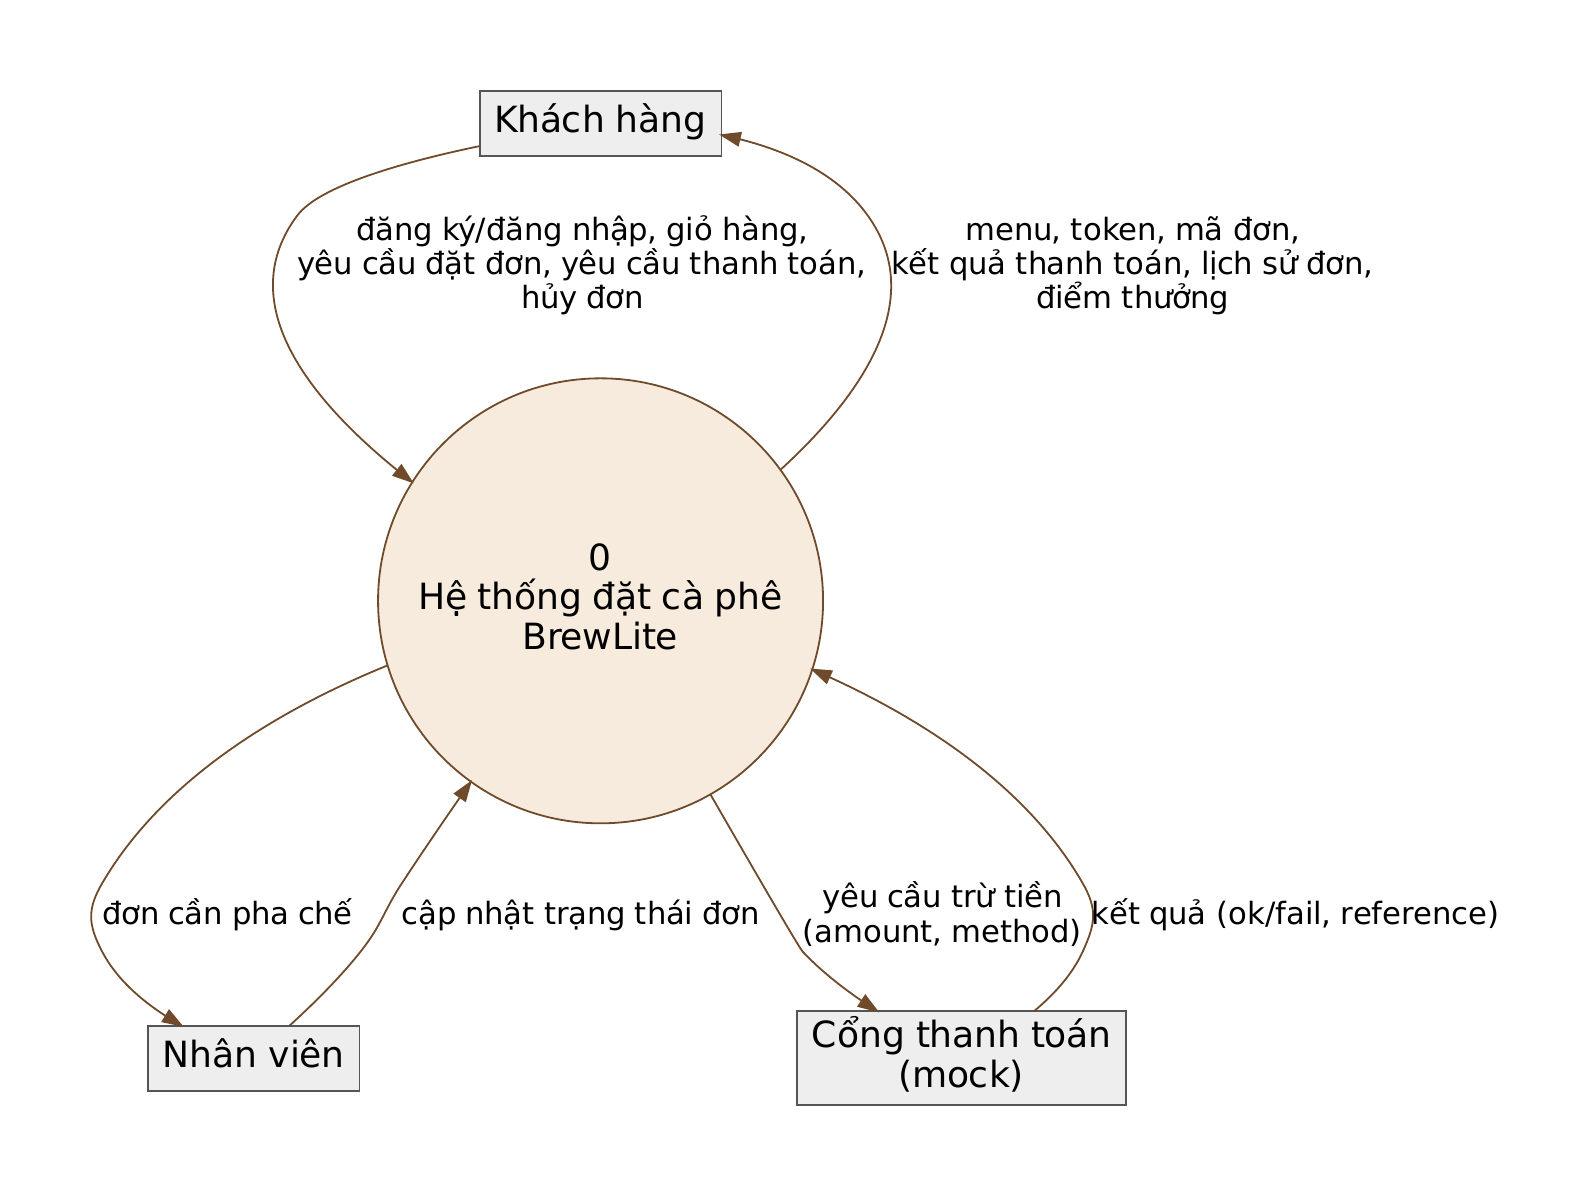
\includegraphics[width=0.47\textwidth,height=0.30\textheight,keepaspectratio]{img/a1/dfd0.png}}\hspace{2mm}
\fbox{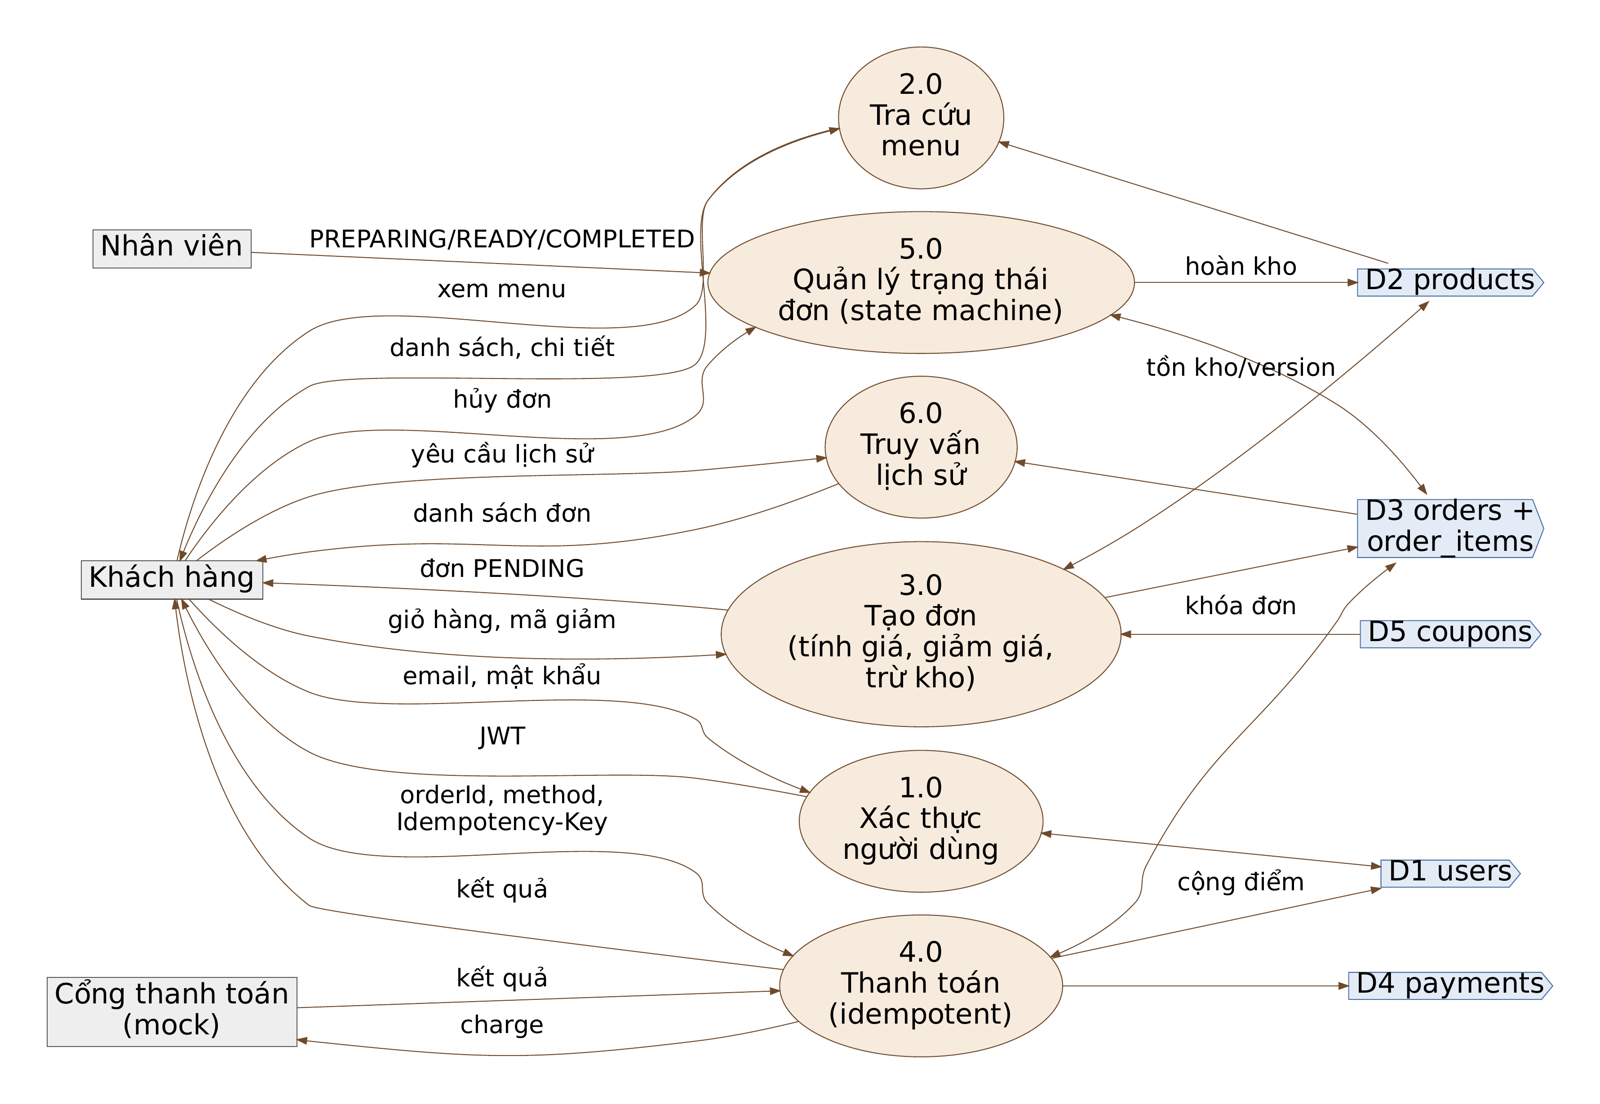
\includegraphics[width=0.47\textwidth,height=0.30\textheight,keepaspectratio]{img/a1/dfd1.png}}\hspace{2mm}
\end{center}\vspace{-2mm}
\qa{43}{\lvA}{DFD mô tả gì? Khác use case và activity thế nào?}{DFD mô tả DỮ LIỆU đi từ đâu, qua xử lý nào, được lưu ở đâu. Use case mô tả ai làm gì; activity mô tả thứ tự bước và điều kiện. DFD không có thứ tự thời gian hay rẽ nhánh.}
\qa{44}{\lvA}{4 ký hiệu của DFD?}{Tác nhân ngoài (hình chữ nhật), tiến trình (hình tròn/chữ nhật bo góc, có số và động từ), kho dữ liệu (hai đường song song hoặc hộp hở, D1, D2...), luồng dữ liệu (mũi tên có nhãn là danh từ).}
\qa{45}{\lvA}{DFD mức 0 (sơ đồ ngữ cảnh) của em có gì?}{Một tiến trình duy nhất '0 Hệ thống BrewLite' và 3 tác nhân ngoài: Khách hàng, Nhân viên, Cổng thanh toán, với các luồng vào/ra như yêu cầu đặt đơn, xác nhận, yêu cầu charge, kết quả thanh toán.}
\qa{46}{\lvA}{DFD mức 1 có những tiến trình và kho nào?}{6 tiến trình: 1.0 Xác thực, 2.0 Tra cứu menu, 3.0 Tạo đơn, 4.0 Thanh toán (idempotent), 5.0 Quản lý trạng thái đơn, 6.0 Truy vấn lịch sử. 5 kho: D1 users, D2 products, D3 orders + order\_items, D4 payments, D5 coupons.}
\qa{47}{\lvB}{Các luật bắt buộc khi vẽ DFD?}{Luồng dữ liệu phải đi qua tiến trình: không nối trực tiếp tác nhân – tác nhân, tác nhân – kho, kho – kho. Mỗi tiến trình có ít nhất một luồng vào và một luồng ra (tránh hố đen, phép màu). Kho phải có luồng vào và ra. Cân bằng: luồng vào/ra mức con khớp với tiến trình cha.}
\qa{48}{\lvB}{Hố đen, phép màu, xám là gì?}{Hố đen: tiến trình chỉ có vào không có ra. Phép màu: chỉ có ra không có vào. Hố xám (grey hole): đầu vào không đủ để tạo ra đầu ra.}
\qa{49}{\lvB}{Cân bằng DFD là gì?}{Khi phân rã tiến trình cha thành mức con, tất cả luồng vào/ra của cha phải xuất hiện ở mức con (cùng tác nhân, cùng dữ liệu). Ví dụ luồng 'yêu cầu đặt đơn' từ Khách hàng ở mức 0 phải có ở mức 1 (vào tiến trình 3.0).}
\qa{50}{\lvC}{Ở A2 bảng coupons đã đổi thành promotions. DFD có cần sửa không?}{Có, kho D5 nên đổi tên thành promotions và thêm kho loyalty\_transactions (D6) nối với tiến trình 4.0 (cộng điểm) và 5.0 (thu hồi khi hủy). Đây là ví dụ cho việc sơ đồ phải được cập nhật qua pull request khi mô hình dữ liệu đổi.}
\section{Sơ đồ hoạt động (Activity)}
\noindent\textit{Activity A1 (2 sơ đồ) và Activity-01 A2 có swimlane.} \hfill \small(7 câu)\normalsize\par\medskip
\begin{center}
\fbox{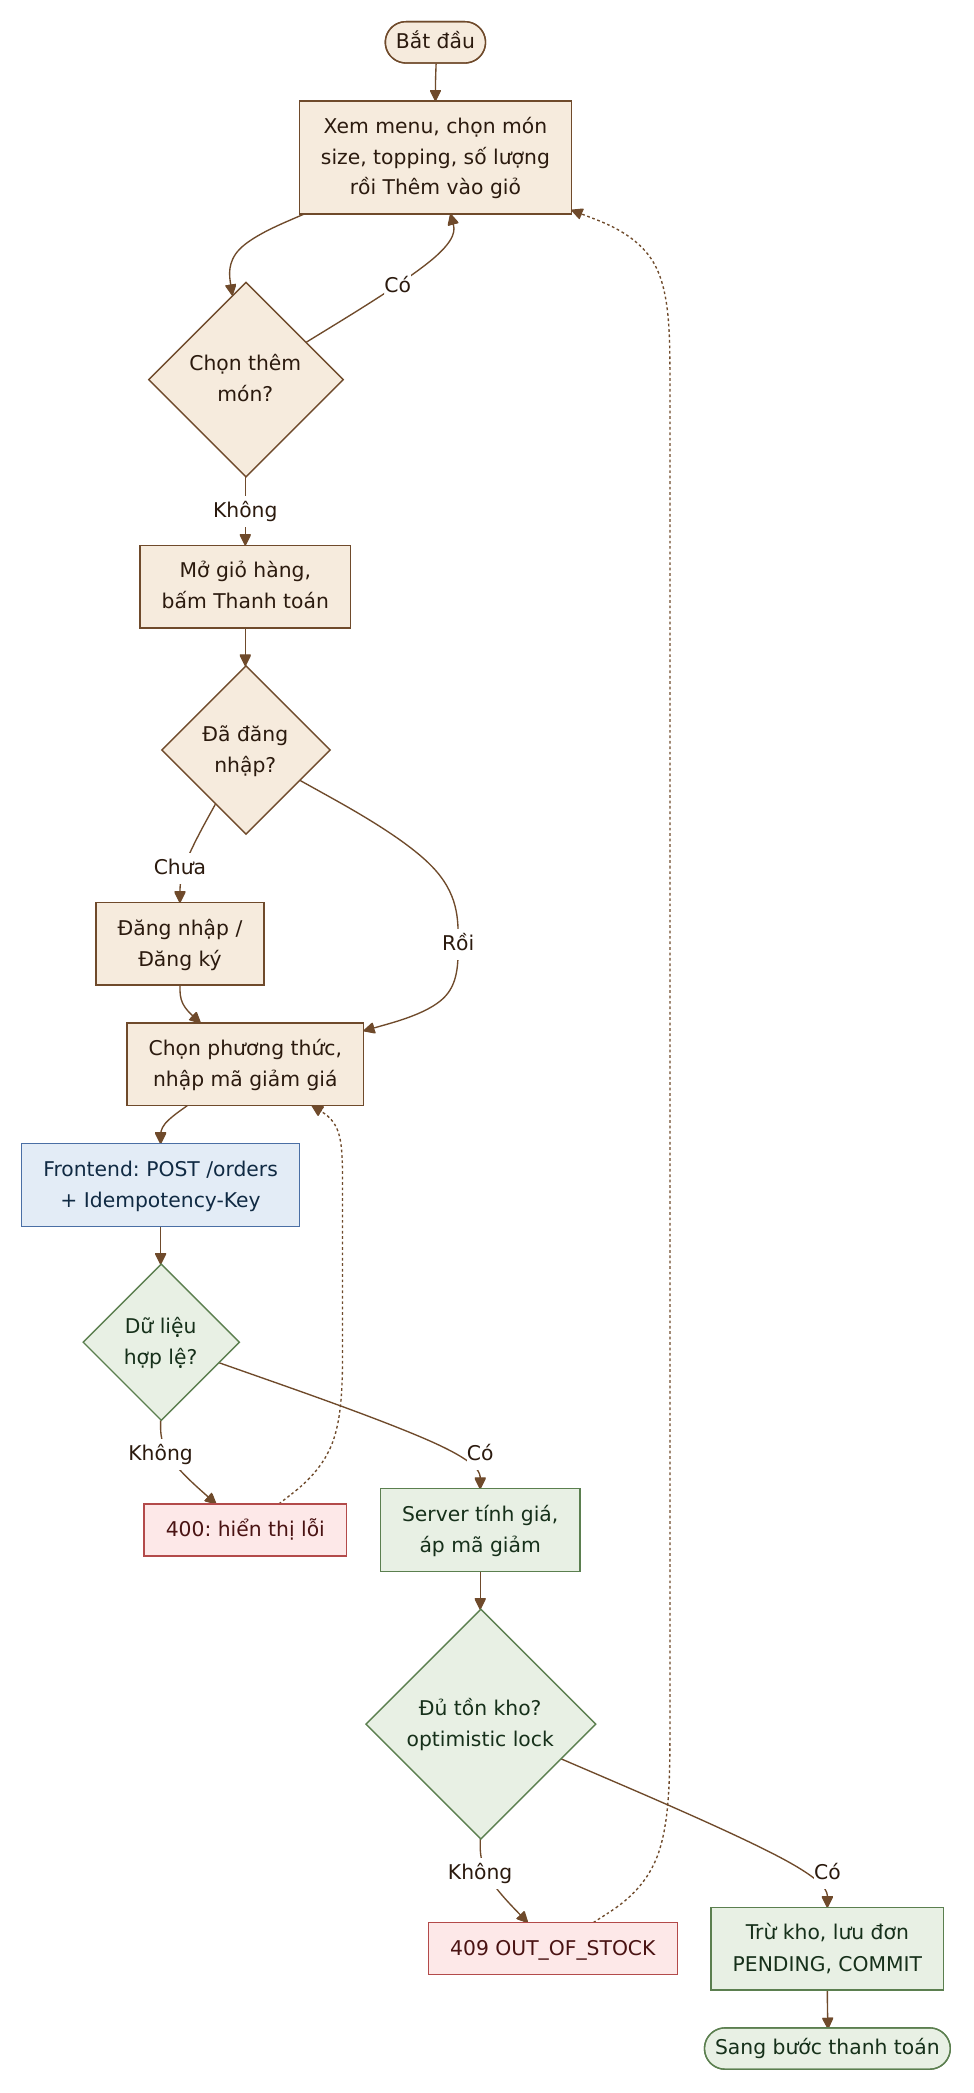
\includegraphics[width=0.47\textwidth,height=0.30\textheight,keepaspectratio]{img/a1/activity-a.png}}\hspace{2mm}
\fbox{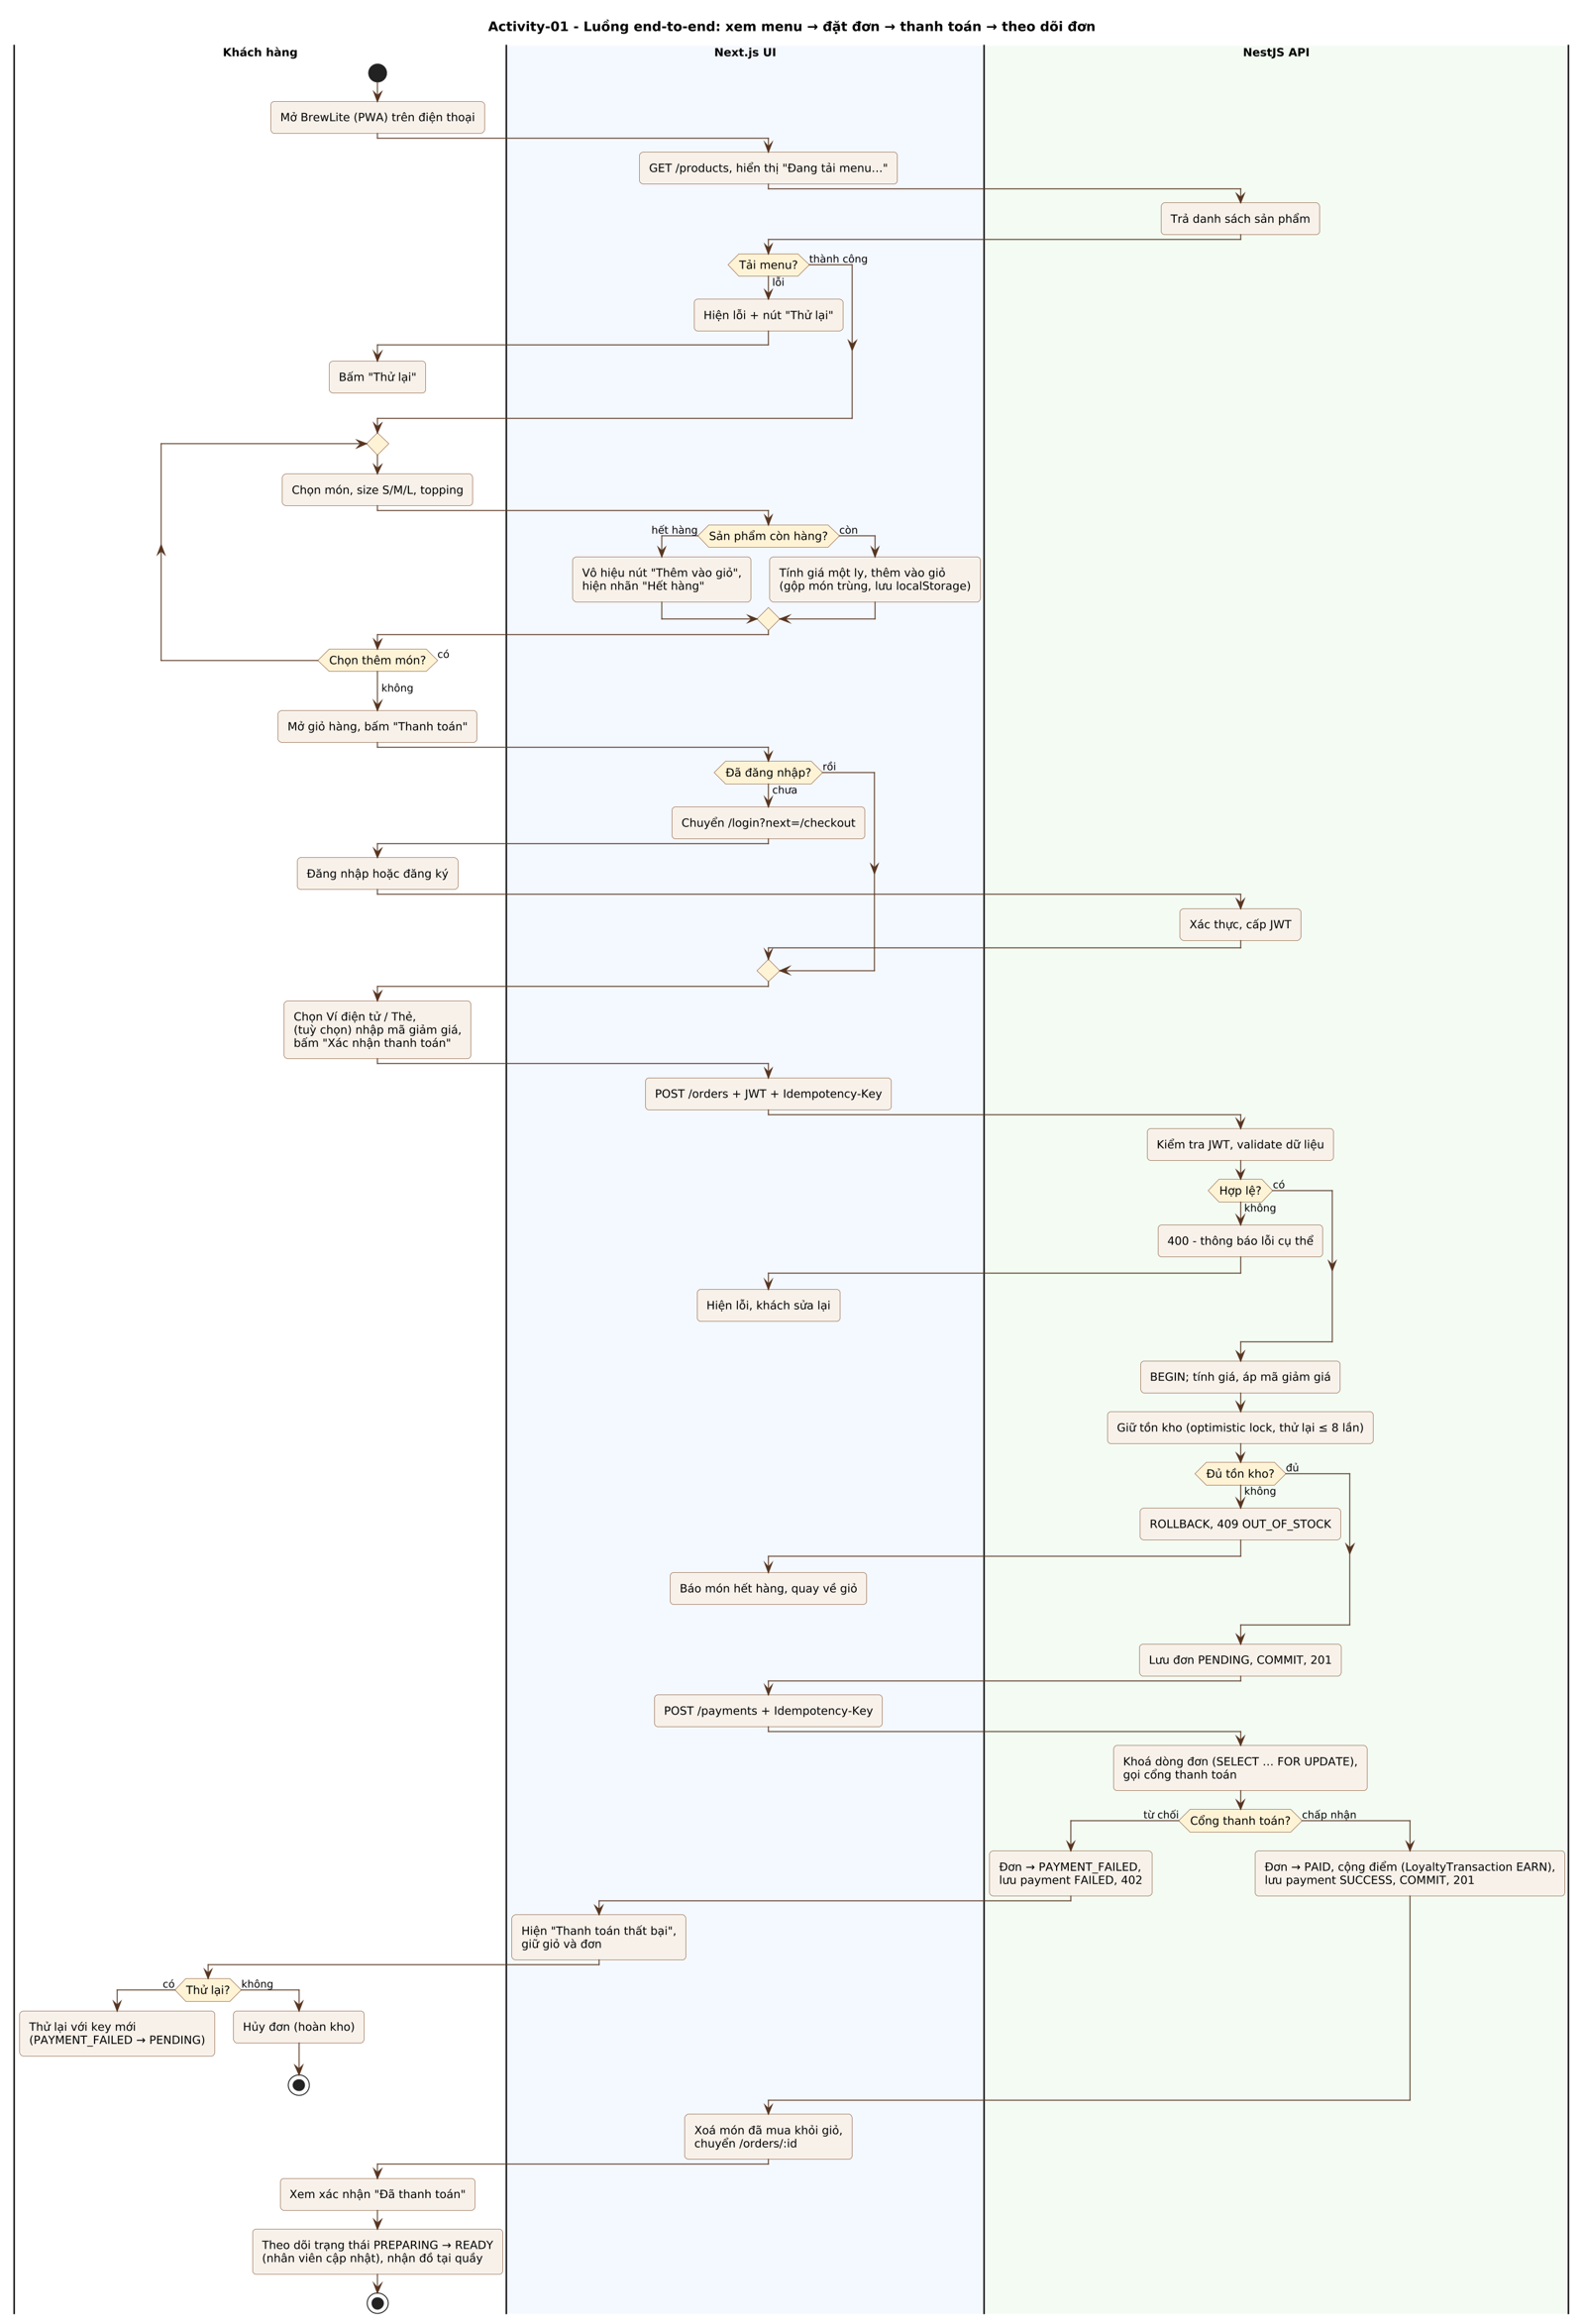
\includegraphics[width=0.47\textwidth,height=0.30\textheight,keepaspectratio]{img/a2/activity-checkout.png}}\hspace{2mm}
\end{center}\vspace{-2mm}
\qa{51}{\lvA}{Activity diagram dùng để làm gì?}{Mô tả luồng công việc từng bước của một quy trình, có rẽ nhánh, hợp nhánh, song song và trách nhiệm từng bên (swimlane).}
\qa{52}{\lvA}{Các ký hiệu của activity diagram?}{Nút bắt đầu (chấm đen), hành động (hình chữ nhật bo góc), decision và merge (hình thoi), fork/join (thanh đen), nút kết thúc hoạt động (chấm đen trong vòng tròn), flow final (vòng tròn có dấu X), swimlane (làn), guard [điều kiện] trên nhánh.}
\qa{53}{\lvA}{Decision khác fork thế nào?}{Decision chọn MỘT nhánh theo điều kiện (if/else). Fork chạy NHIỀU nhánh song song, join chờ tất cả xong mới đi tiếp.}
\qa{54}{\lvB}{Activity-01 của A2 có những swimlane nào và đủ 3 trường hợp đề yêu cầu chưa?}{3 làn: Khách hàng, Next.js UI, NestJS API. Có đủ: hết hàng (ở bước chọn món: vô hiệu nút; ở bước giữ kho: 409 OUT\_OF\_STOCK), chưa đăng nhập (chuyển /login?next=/checkout), thanh toán thất bại (PAYMENT\_FAILED, chọn thử lại hoặc hủy). Thêm lỗi tải menu và dữ liệu sai 400.}
\qa{55}{\lvB}{Kể luồng hoạt động end-to-end theo Activity-01.}{Mở app $\rightarrow$ UI gọi GET /products (lỗi thì Thử lại) $\rightarrow$ khách chọn món, size, topping (hết hàng thì không thêm được) $\rightarrow$ thêm giỏ, lặp lại nếu chọn thêm $\rightarrow$ bấm Thanh toán $\rightarrow$ chưa đăng nhập thì đăng nhập/đăng ký $\rightarrow$ chọn phương thức, nhập mã $\rightarrow$ POST /orders $\rightarrow$ API validate (sai 400) $\rightarrow$ BEGIN, tính giá, giữ kho (thiếu 409) $\rightarrow$ lưu PENDING $\rightarrow$ POST /payments $\rightarrow$ khóa đơn, gọi cổng $\rightarrow$ từ chối: PAYMENT\_FAILED (thử lại hoặc hủy) / chấp nhận: PAID, cộng điểm $\rightarrow$ xóa giỏ, /orders/:id $\rightarrow$ theo dõi PREPARING $\rightarrow$ READY $\rightarrow$ nhận tại quầy.}
\qa{56}{\lvB}{Guard condition là gì? Yêu cầu gì với các nhánh?}{Điều kiện trong ngoặc vuông trên nhánh ra của decision, ví dụ [đủ tồn kho]. Các guard phải loại trừ nhau và bao phủ mọi trường hợp (không có trường hợp không nhánh nào đúng).}
\qa{57}{\lvA}{Khi nào dùng swimlane?}{Khi quy trình có nhiều actor hoặc thành phần chịu trách nhiệm khác nhau, để thấy rõ bước nào do ai làm (khách, frontend, backend).}
\section{Sơ đồ tuần tự (Sequence)}
\noindent\textit{5 sequence A1 (auth, tạo đơn, thanh toán, hủy, race) và Sequence-01 A2.} \hfill \small(11 câu)\normalsize\par\medskip
\begin{center}
\fbox{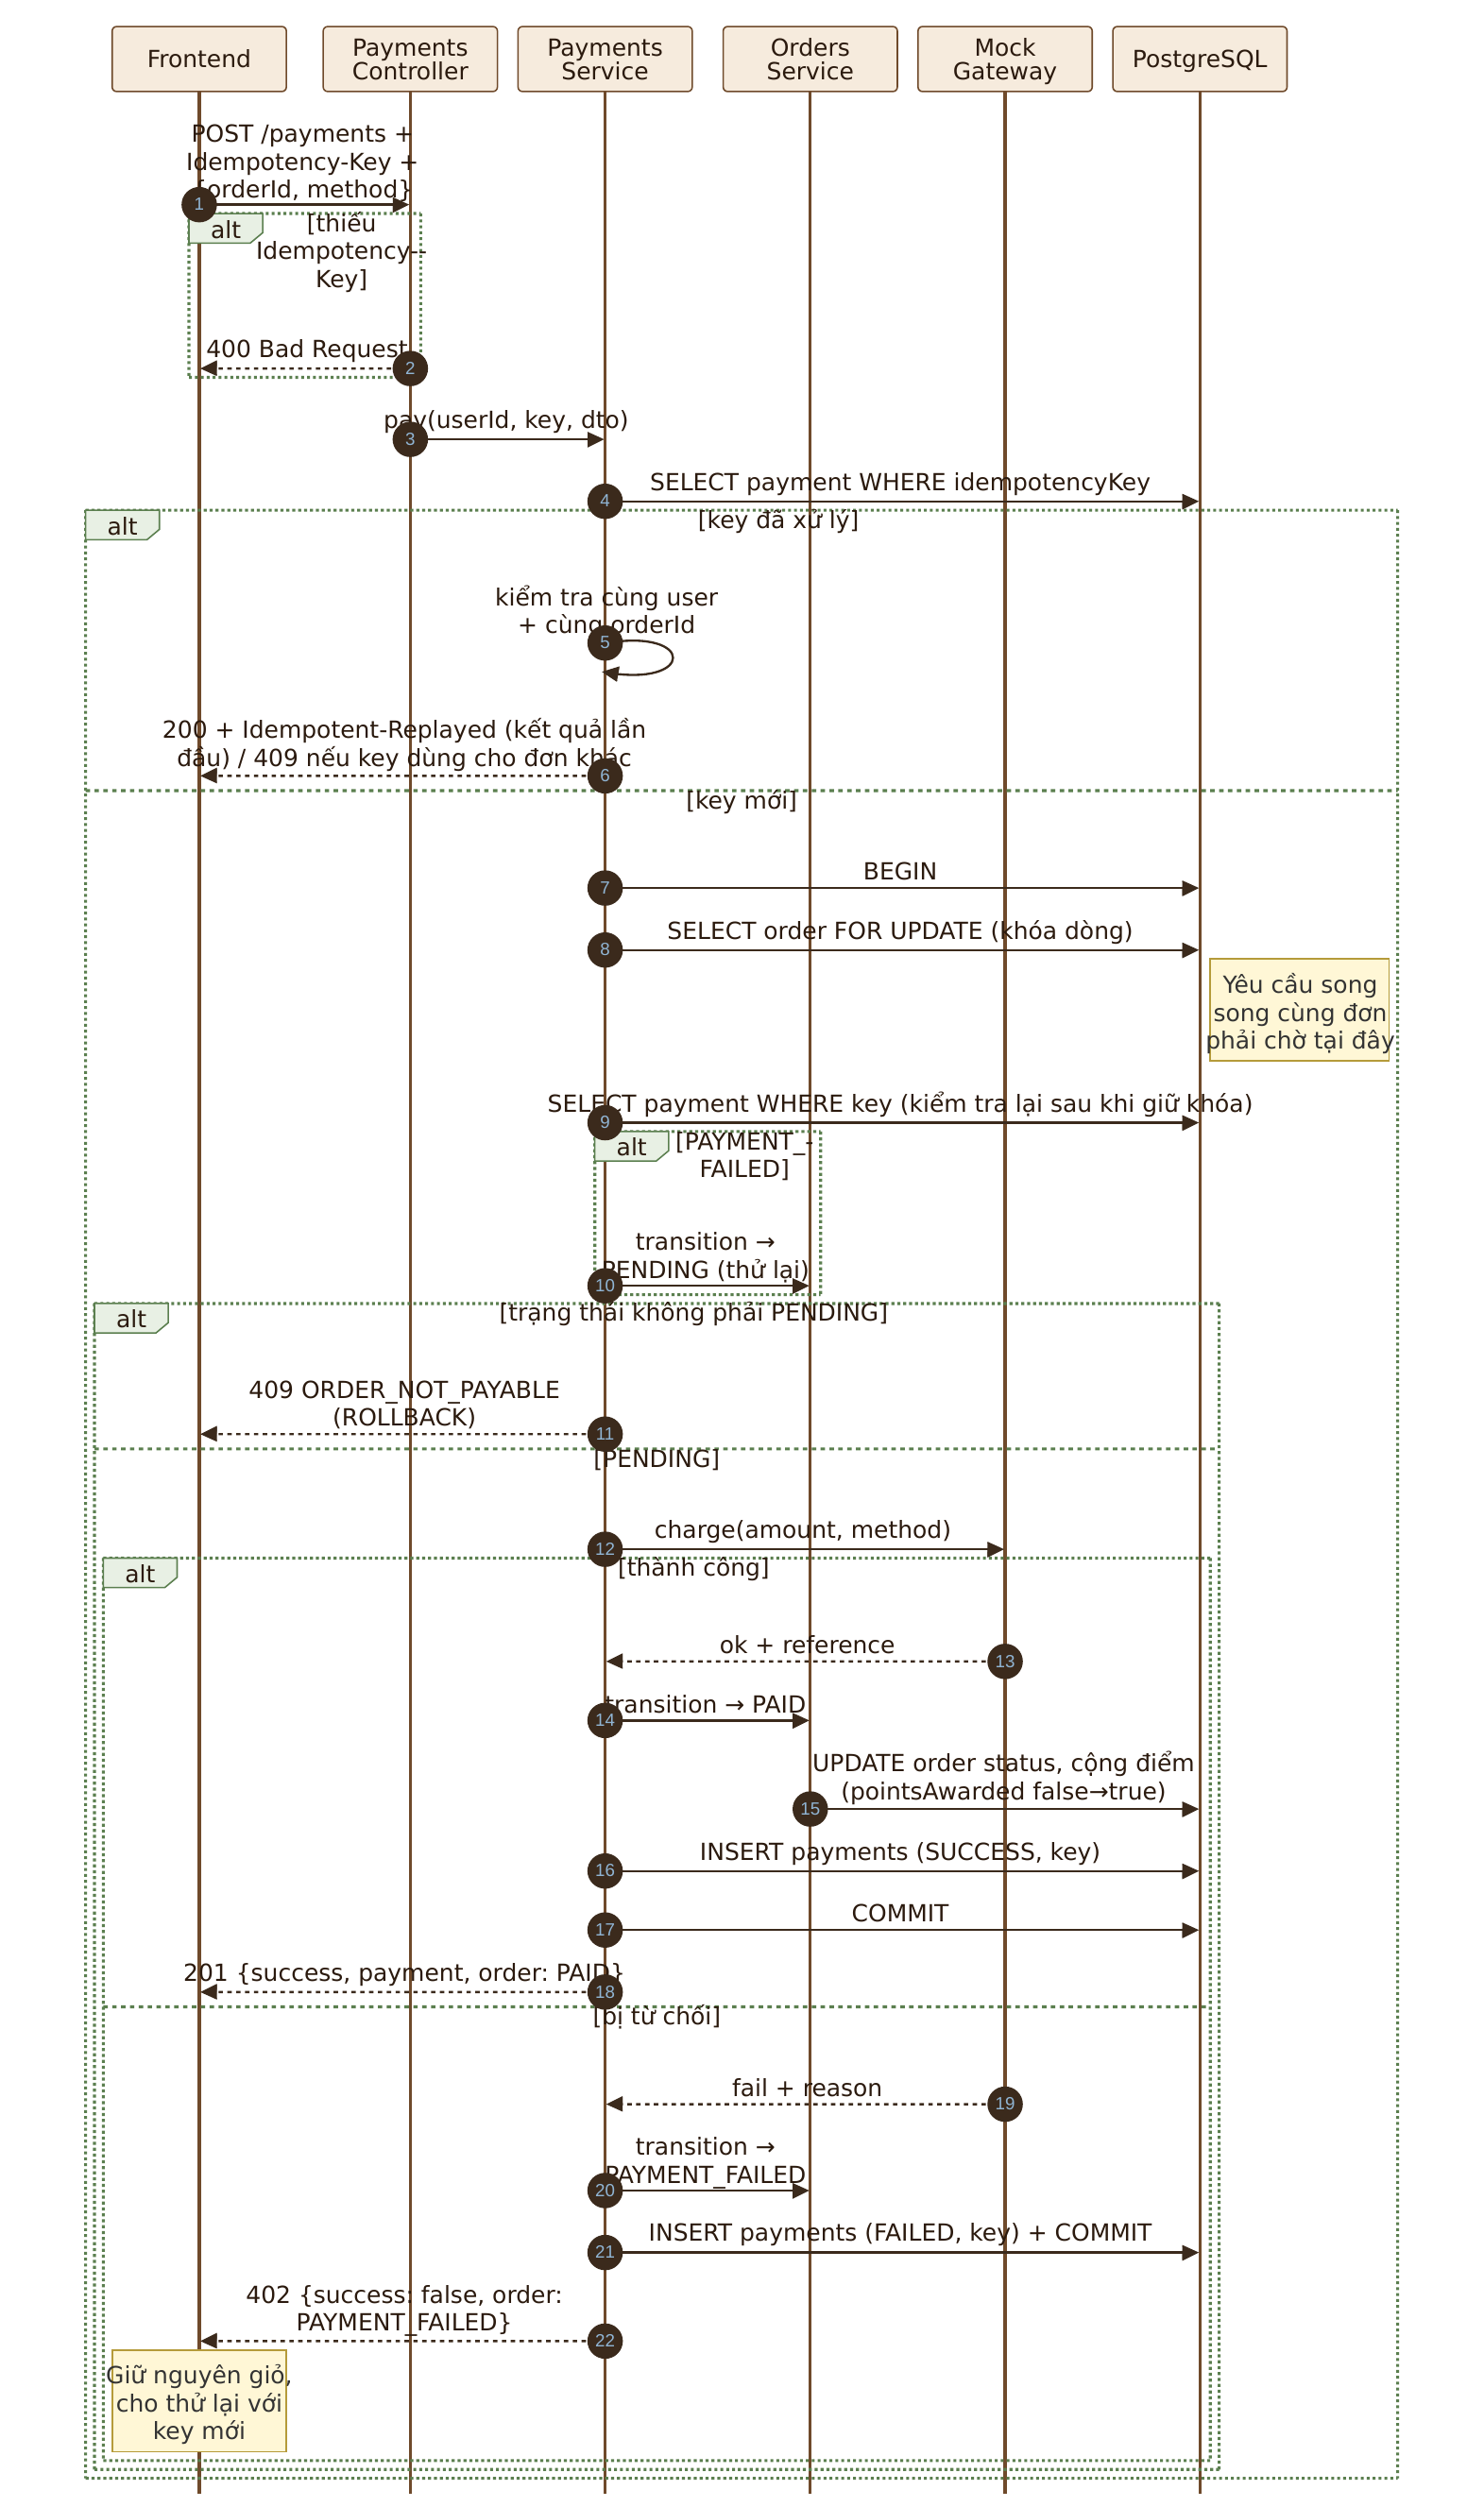
\includegraphics[width=0.47\textwidth,height=0.30\textheight,keepaspectratio]{img/a1/seq-pay.png}}\hspace{2mm}
\fbox{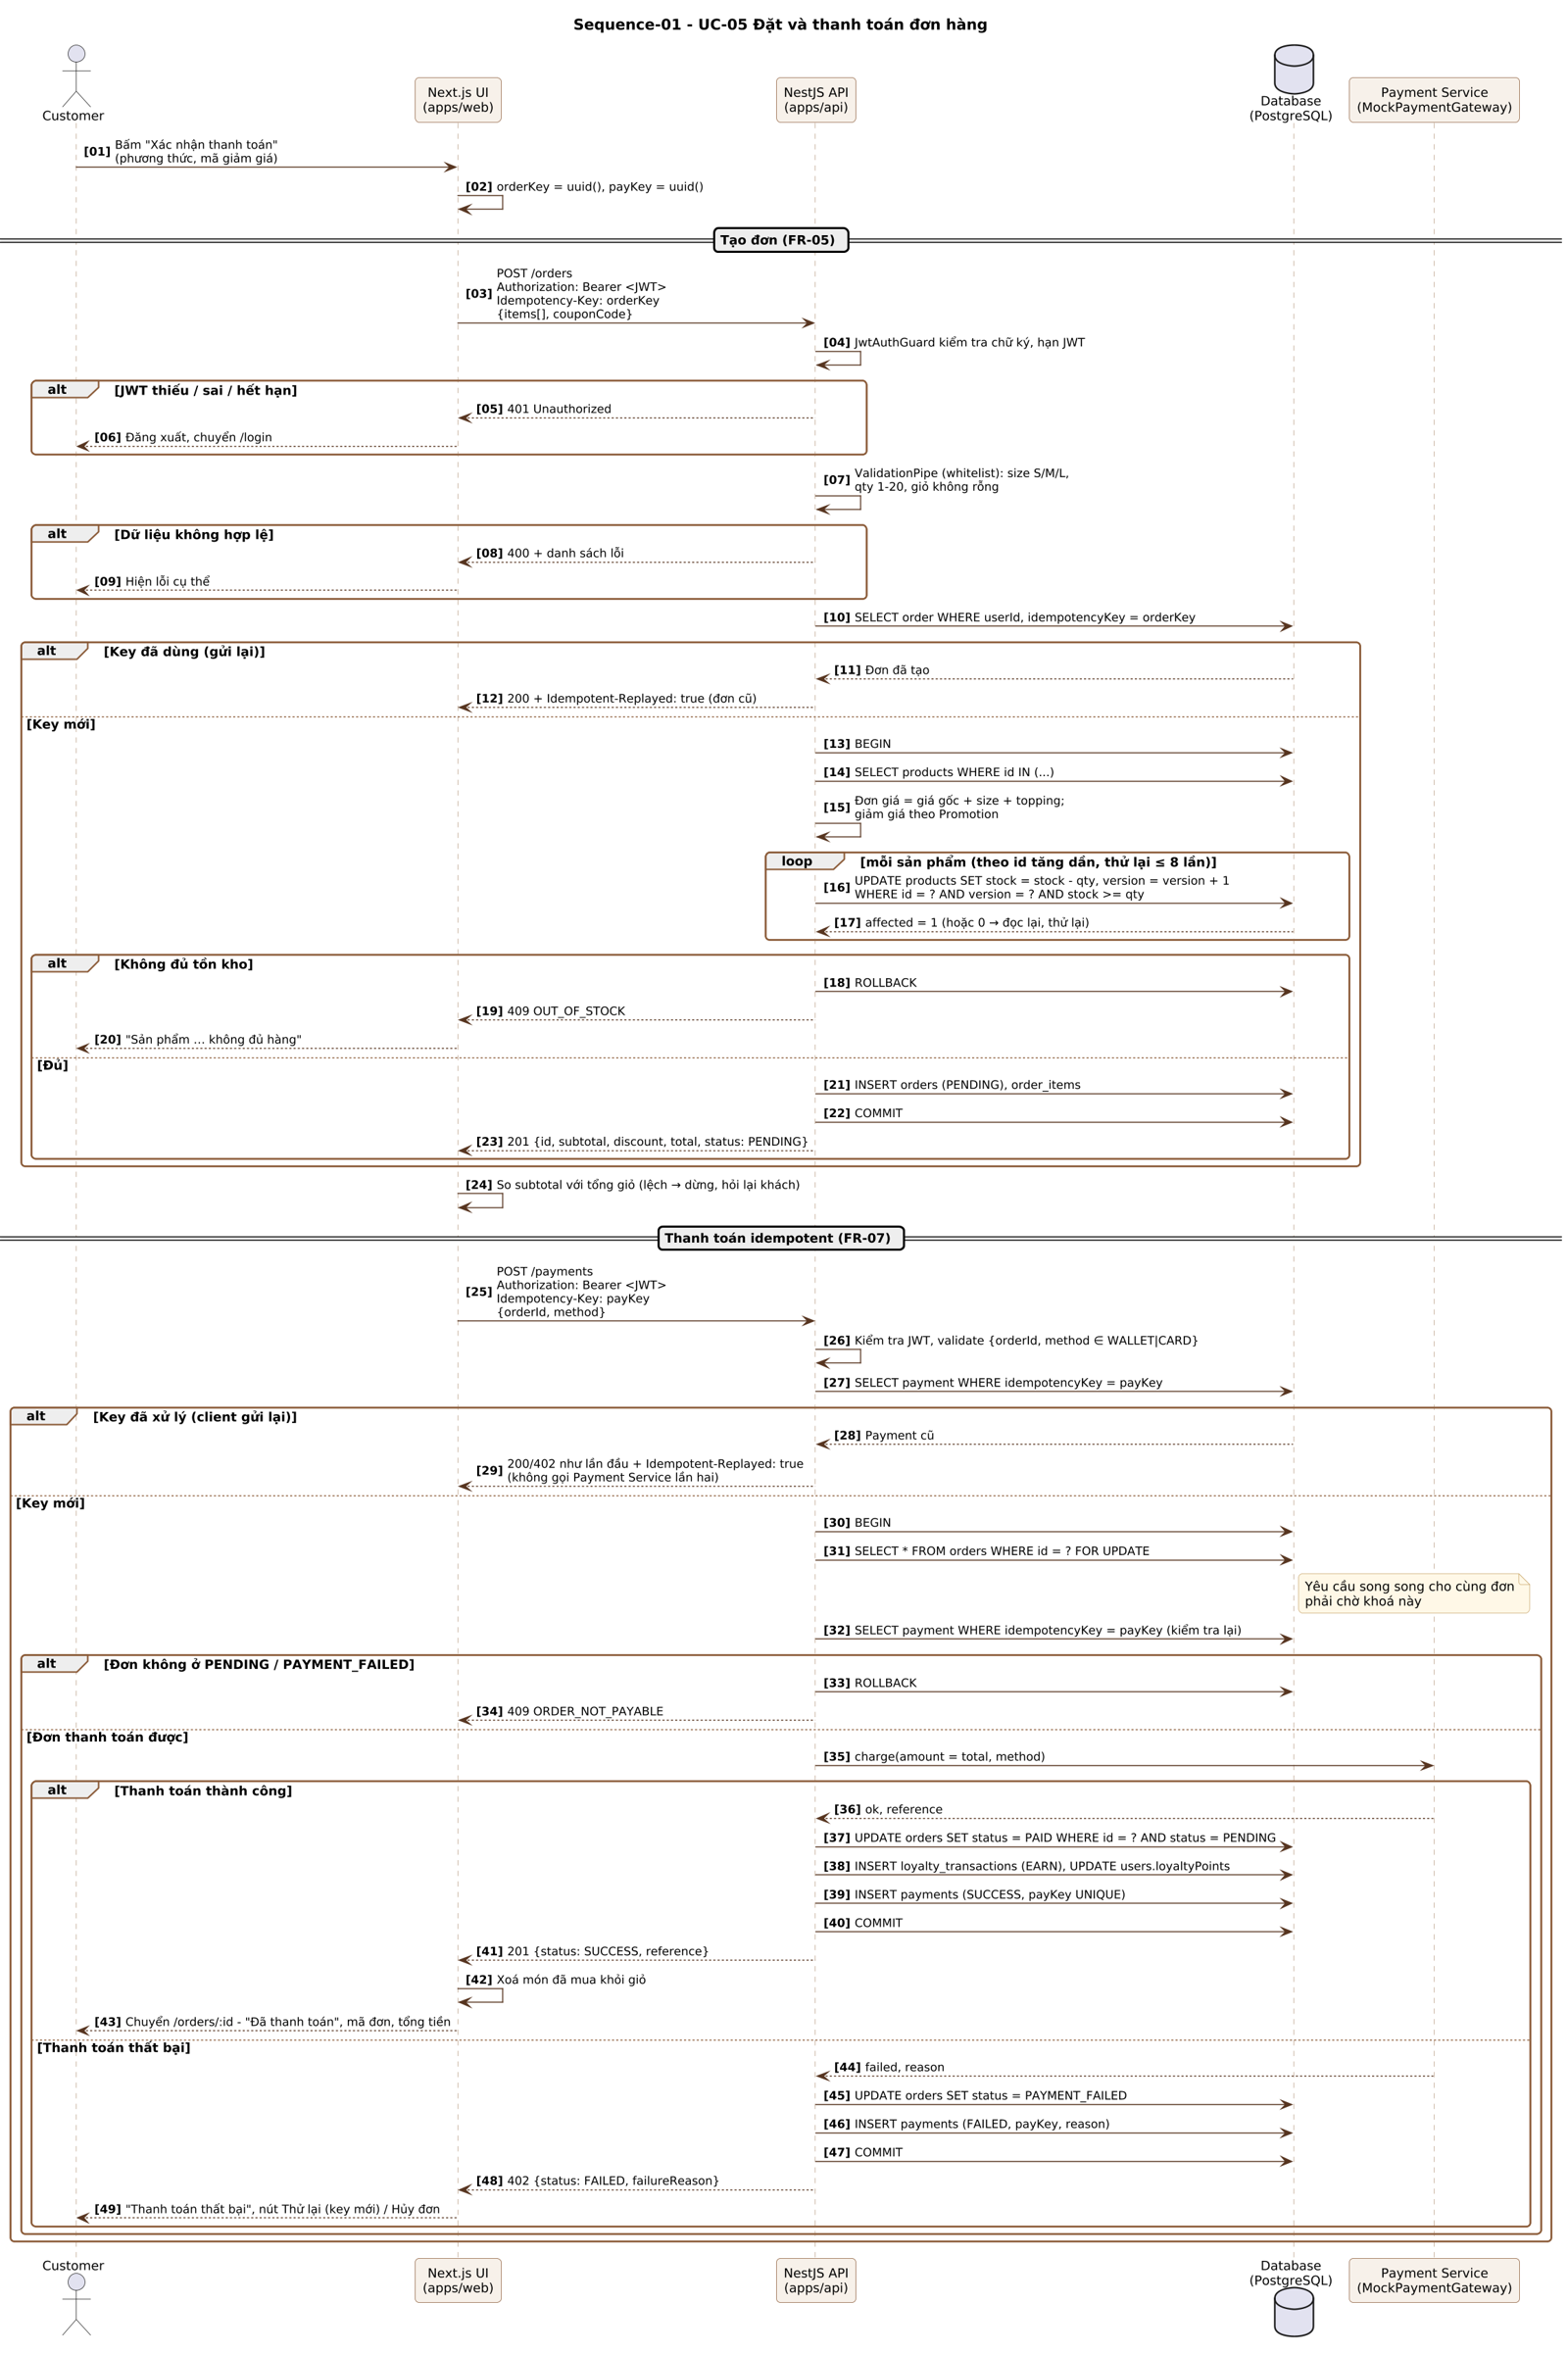
\includegraphics[width=0.47\textwidth,height=0.30\textheight,keepaspectratio]{img/a2/sequence-checkout.png}}\hspace{2mm}
\end{center}\vspace{-2mm}
\qa{58}{\lvA}{Sequence diagram mô tả gì?}{Các đối tượng trao đổi thông điệp theo thứ tự thời gian (từ trên xuống) trong MỘT kịch bản cụ thể.}
\qa{59}{\lvA}{Các thành phần của sequence diagram?}{Lifeline (đường đứt dọc dưới participant/actor), thanh kích hoạt, thông điệp đồng bộ (mũi tên liền đầu đặc), thông điệp trả về (mũi tên đứt), self-message, fragment alt/opt/loop/par, note, autonumber.}
\qa{60}{\lvA}{alt, opt, loop khác nhau thế nào?}{alt: chọn một trong nhiều nhánh (if/else). opt: một nhánh có thể xảy ra hoặc không (if không else). loop: lặp lại. par: chạy song song.}
\qa{61}{\lvA}{5 lifeline bắt buộc trong Sequence-01 A2?}{Customer $\rightarrow$ Next.js UI $\rightarrow$ NestJS API $\rightarrow$ Database $\rightarrow$ Payment Service.}
\qa{62}{\lvB}{Sequence-01 thể hiện kiểm tra JWT và validate ở đâu?}{Ngay khi API nhận POST /orders: JwtAuthGuard kiểm tra chữ ký và hạn token (alt 401), ValidationPipe whitelist kiểm tra size S/M/L, qty 1–20, giỏ không rỗng (alt 400). Tương tự ở POST /payments.}
\qa{63}{\lvB}{Transaction tạo đơn được vẽ thế nào?}{BEGIN $\rightarrow$ SELECT products $\rightarrow$ tính đơn giá, giảm giá $\rightarrow$ loop mỗi sản phẩm (theo id tăng dần, thử lại $\le$ 8): UPDATE products SET stock = stock $-$ qty, version = version + 1 WHERE id = ? AND version = ? AND stock \textgreater{}= qty $\rightarrow$ alt không đủ: ROLLBACK, 409; đủ: INSERT orders + order\_items, COMMIT, 201.}
\qa{64}{\lvB}{Idempotency thể hiện ở đâu trong sequence?}{Trước khi xử lý, API tìm payment theo Idempotency-Key. Đã có thì trả kết quả cũ (200/402 + header Idempotent-Replayed: true) và KHÔNG gọi Payment Service. Key mới thì BEGIN, SELECT ... FOR UPDATE khóa dòng đơn, kiểm tra lại key rồi mới gọi cổng.}
\qa{65}{\lvB}{Sequence thanh toán: thành công và thất bại khác nhau thế nào?}{Thành công: UPDATE orders $\rightarrow$ PAID, INSERT loyalty\_transactions EARN + tăng điểm, INSERT payments SUCCESS, COMMIT, 201. Thất bại: UPDATE orders $\rightarrow$ PAYMENT\_FAILED, INSERT payments FAILED (kèm lý do), COMMIT, 402, không cộng điểm.}
\qa{66}{\lvB}{Sequence race (A1) minh họa điều gì?}{Hai khách cùng mua sản phẩm cuối cùng. Cả hai đọc stock = 1, version = n. Người A cập nhật thành công (version $\rightarrow$ n+1). Người B UPDATE với version = n không khớp nên 0 dòng bị ảnh hưởng $\rightarrow$ đọc lại thấy stock = 0 $\rightarrow$ 409 OUT\_OF\_STOCK. Không ai làm kho âm.}
\qa{67}{\lvB}{Sequence hủy đơn (A1) có gì?}{Khách POST /orders/:id/cancel $\rightarrow$ OrdersService kiểm tra quyền, assertTransition(status, CANCELLED) (self-message) $\rightarrow$ UPDATE ... WHERE status = \textless{}hiện tại\textgreater{} $\rightarrow$ hoàn kho (release) $\rightarrow$ nếu đã PAID thì thu hồi điểm $\rightarrow$ trả 201. Nhân viên PATCH /orders/:id/status chuyển PREPARING $\rightarrow$ READY $\rightarrow$ COMPLETED.}
\qa{68}{\lvC}{Vì sao khóa dòng đơn khi thanh toán mà không dùng optimistic lock?}{Thanh toán chỉ trên MỘT đơn, ít tranh chấp nhưng cần tuần tự tuyệt đối và có gọi cổng ngoài. Khóa bi quan (FOR UPDATE) bắt các request song song cùng đơn phải chờ, tránh gọi cổng hai lần. Tồn kho thì nhiều đơn tranh chấp, mỗi lần cập nhật rất ngắn, nên dùng optimistic lock để có thông lượng tốt.}
\section{Sơ đồ lớp (Class)}
\noindent\textit{Class domain + class service A1, Class-01 A2 có Promotion và LoyaltyTransaction.} \hfill \small(11 câu)\normalsize\par\medskip
\begin{center}
\fbox{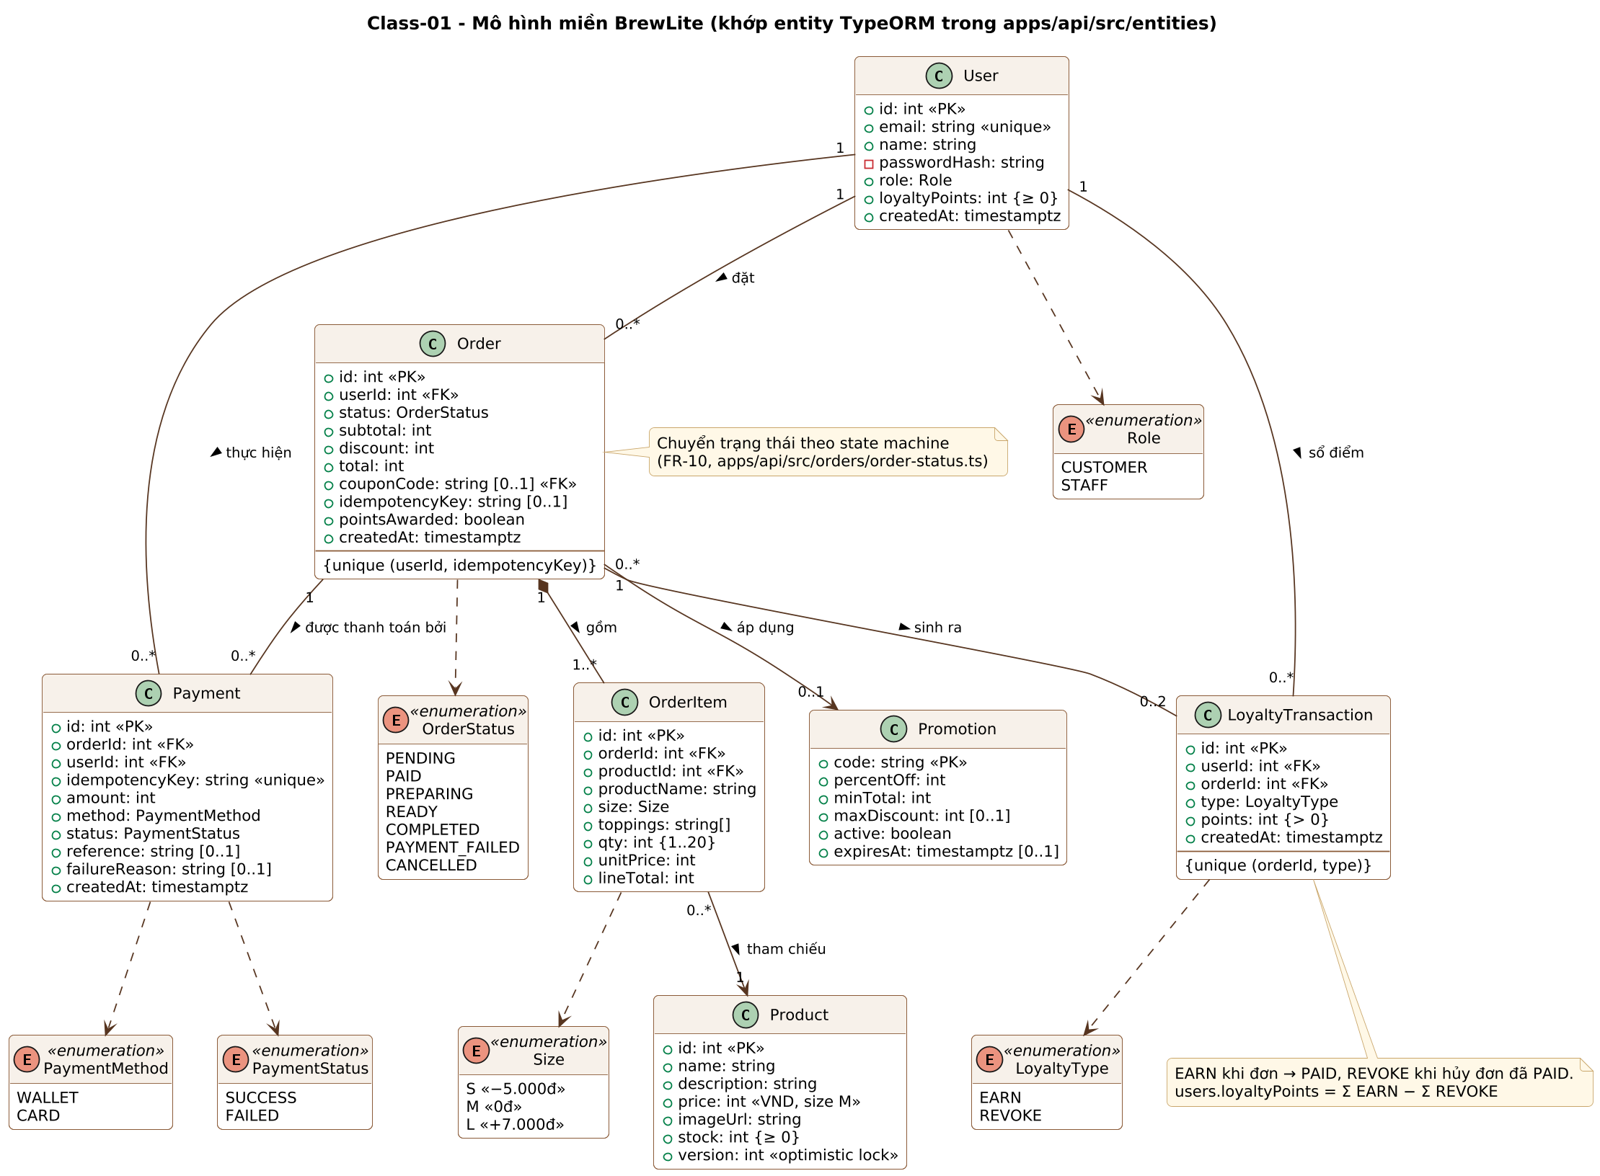
\includegraphics[width=0.47\textwidth,height=0.30\textheight,keepaspectratio]{img/a2/class-domain.png}}\hspace{2mm}
\fbox{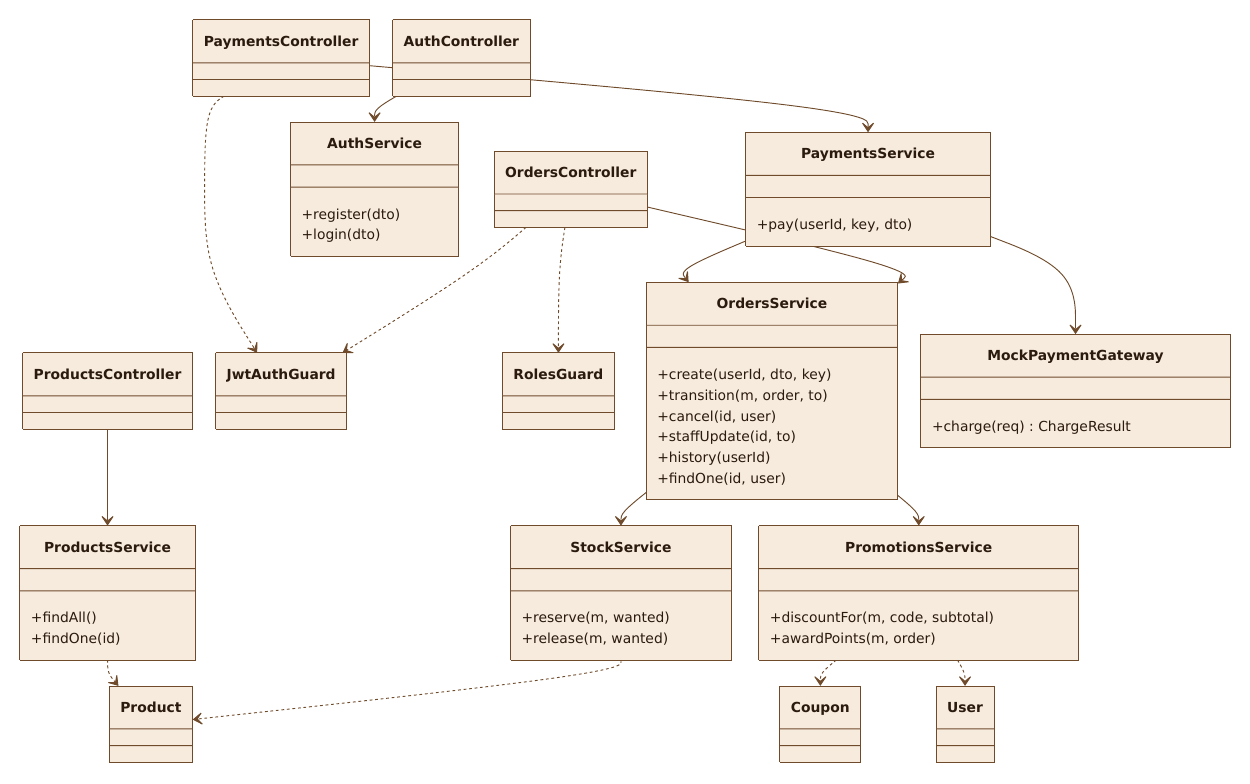
\includegraphics[width=0.47\textwidth,height=0.30\textheight,keepaspectratio]{img/a1/class-service.png}}\hspace{2mm}
\end{center}\vspace{-2mm}
\qa{69}{\lvA}{Class diagram mô tả gì?}{Cấu trúc tĩnh: các lớp, thuộc tính, phương thức và quan hệ giữa chúng.}
\qa{70}{\lvA}{Một lớp gồm mấy ngăn? Các ký hiệu phạm vi?}{3 ngăn: tên lớp, thuộc tính, phương thức. + public, - private, \# protected, \textasciitilde{} package.}
\qa{71}{\lvA}{Các loại quan hệ trong class diagram?}{Association (đường liền), aggregation (thoi rỗng, phần sống độc lập), composition (thoi đặc, phần chết theo tổng thể), dependency (mũi tên đứt), generalization (mũi tên liền đầu tam giác rỗng – kế thừa), realization (mũi tên đứt đầu tam giác rỗng – cài đặt interface).}
\qa{72}{\lvB}{Aggregation và composition khác nhau thế nào? Ví dụ trong đồ án.}{Composition: phần không tồn tại ngoài tổng thể, xóa tổng thể thì phần mất theo – Order *-- OrderItem. Aggregation: phần có thể tồn tại độc lập. OrderItem chỉ THAM CHIẾU Product (association có hướng), xóa đơn không xóa sản phẩm.}
\qa{73}{\lvA}{7 lớp bắt buộc của Class-01 A2 và enum?}{User, Product, Order, OrderItem, Payment, Promotion, LoyaltyTransaction. Enum: OrderStatus (7), Role (CUSTOMER, STAFF), PaymentMethod (WALLET, CARD), PaymentStatus (SUCCESS, FAILED), LoyaltyType (EARN, REVOKE), Size (S, M, L).}
\qa{74}{\lvB}{Đọc bội số các quan hệ chính.}{User 1 — 0..* Order; Order 1 *-- 1..* OrderItem; OrderItem 0..* $\rightarrow$ 1 Product; Order 1 — 0..* Payment; User 1 — 0..* Payment; Order 0..* $\rightarrow$ 0..1 Promotion; User 1 — 0..* LoyaltyTransaction; Order 1 — 0..2 LoyaltyTransaction.}
\qa{75}{\lvC}{Vì sao Order — LoyaltyTransaction là 0..2?}{Ràng buộc UNIQUE(orderId, type): mỗi đơn có tối đa một dòng EARN (khi PAID) và một dòng REVOKE (khi hủy đơn đã PAID). Đơn chưa thanh toán có 0 dòng.}
\qa{76}{\lvA}{Vì sao passwordHash là private (-)?}{Đây là dữ liệu nhạy cảm, không được lộ ra ngoài lớp/API. Thực tế API không bao giờ trả trường này.}
\qa{77}{\lvB}{Vì sao OrderItem lưu productName và unitPrice thay vì chỉ productId?}{Để giữ giá và tên TẠI THỜI ĐIỂM ĐẶT. Nếu sau này đổi giá hoặc tên sản phẩm, đơn cũ vẫn đúng như lúc khách trả tiền (dữ liệu lịch sử).}
\qa{78}{\lvB}{Class diagram service (A1) cho thấy gì?}{Kiến trúc controller $\rightarrow$ service: AuthController $\rightarrow$ AuthService, OrdersController $\rightarrow$ OrdersService, PaymentsController $\rightarrow$ PaymentsService; OrdersService dùng StockService (reserve/release) và PromotionsService (discountFor/awardPoints); PaymentsService dùng OrdersService và MockPaymentGateway; controller phụ thuộc JwtAuthGuard và RolesGuard.}
\qa{79}{\lvB}{Class diagram khác ERD thế nào?}{Class mô tả đối tượng trong code: có phương thức, kế thừa, enum, quan hệ composition. ERD mô tả bảng trong CSDL: khóa chính, khóa ngoại, kiểu dữ liệu, bội số theo ký hiệu chân chim, bảng trung gian cho N-N.}
\section{ERD và cơ sở dữ liệu}
\noindent\textit{ERD A1 và thay đổi ở A2 (promotions, loyalty\_transactions, FK, CHECK, migration).} \hfill \small(10 câu)\normalsize\par\medskip
\begin{center}
\fbox{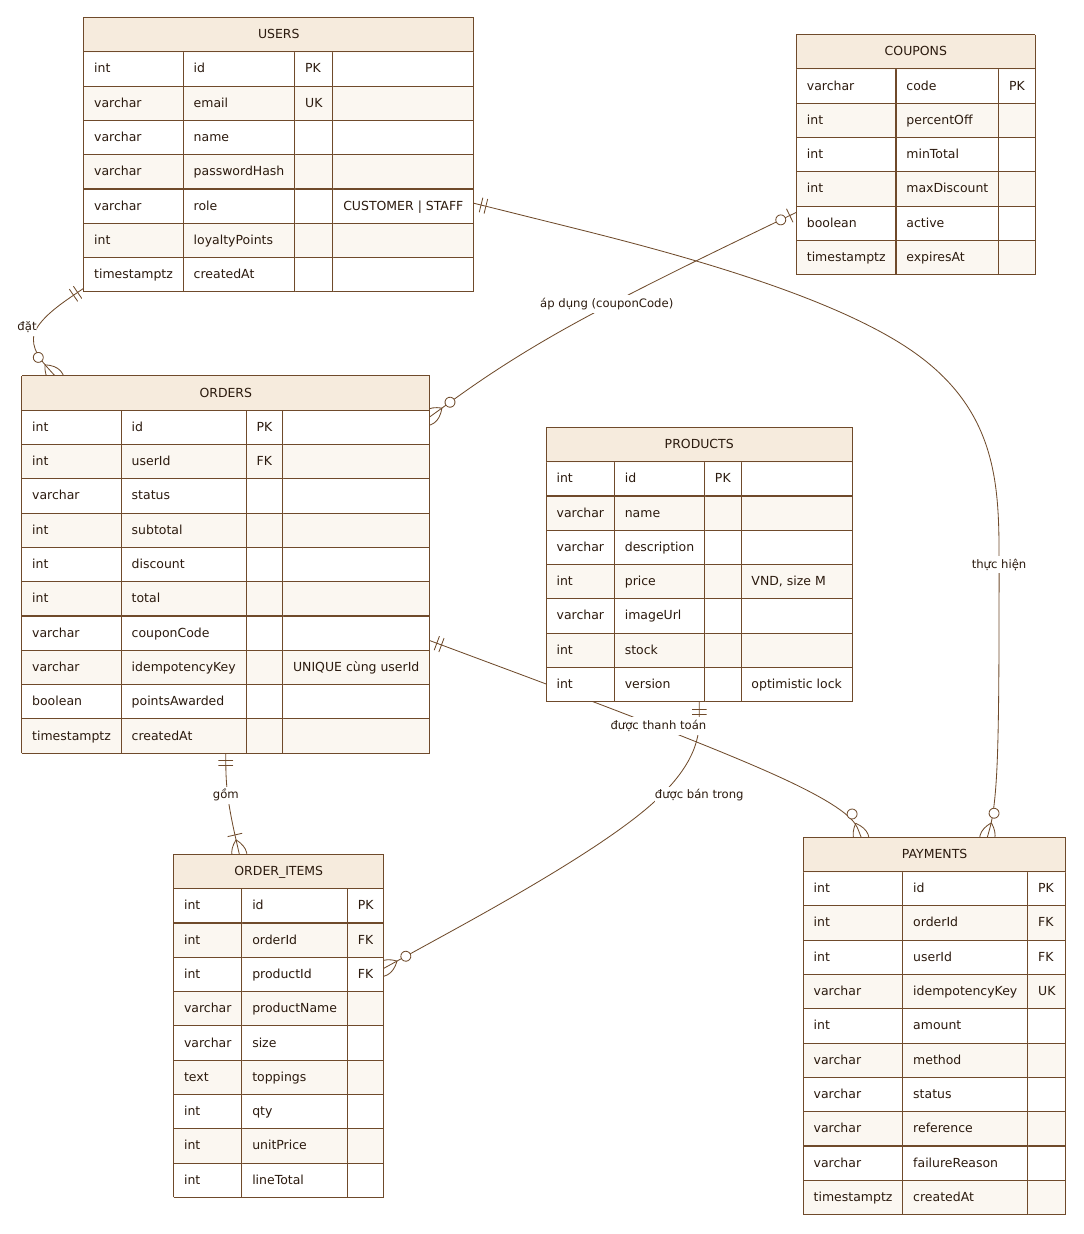
\includegraphics[width=0.62\textwidth,height=0.30\textheight,keepaspectratio]{img/a1/erd.png}}\hspace{2mm}
\end{center}\vspace{-2mm}
\qa{80}{\lvA}{Các bảng trong CSDL BrewLite hiện tại?}{users, products, orders, order\_items, payments, promotions (A1 là coupons), loyalty\_transactions (mới ở A2), và bảng migrations do TypeORM quản lý.}
\qa{81}{\lvA}{PK, FK, UNIQUE khác nhau thế nào?}{PK định danh duy nhất một dòng. FK trỏ tới PK của bảng khác để giữ toàn vẹn tham chiếu. UNIQUE bắt giá trị không trùng nhưng không phải khóa chính (ví dụ users.email, payments.idempotencyKey).}
\qa{82}{\lvA}{Ký hiệu chân chim đọc thế nào?}{| là đúng một, o là không (tùy chọn), chân chim là nhiều. ||--o\{ : một bắt buộc tới không hoặc nhiều. ||--|\{ : một tới một hoặc nhiều.}
\qa{83}{\lvA}{Quan hệ 1-N thì đặt FK ở đâu? N-N thì sao?}{1-N: FK ở bảng phía N (orders.userId). N-N: tạo bảng trung gian chứa hai FK (ví dụ nếu một sản phẩm nhiều danh mục và ngược lại thì cần product\_categories).}
\qa{84}{\lvB}{Các ràng buộc toàn vẹn quan trọng trong CSDL?}{UNIQUE(payments.idempotencyKey); UNIQUE(orders.userId, idempotencyKey); UNIQUE(loyalty\_transactions.orderId, type); UNIQUE(users.email); CHECK(stock \textgreater{}= 0); CHECK(loyaltyPoints \textgreater{}= 0); khóa ngoại orders $\rightarrow$ users/promotions, order\_items $\rightarrow$ orders/products, payments $\rightarrow$ orders/users, loyalty\_transactions $\rightarrow$ users/orders.}
\qa{85}{\lvB}{Vì sao vừa kiểm tra trong code vừa đặt ràng buộc ở CSDL?}{Phòng thủ nhiều lớp. Code có thể có lỗi hoặc có đường ghi dữ liệu khác (script, test); CSDL là lớp cuối cùng bảo đảm không bao giờ có tồn kho âm, payment trùng key hay tham chiếu tới dòng không tồn tại.}
\qa{86}{\lvB}{Cột version trong products dùng để làm gì?}{Optimistic locking: mỗi lần trừ kho tăng version; UPDATE chỉ thành công khi version chưa bị ai đổi (WHERE version = ?). Nếu 0 dòng bị ảnh hưởng nghĩa là có người cập nhật trước $\rightarrow$ đọc lại và thử lại.}
\qa{87}{\lvB}{Migration là gì? Vì sao bỏ synchronize?}{Migration là tệp mô tả từng bước thay đổi schema (up) và cách hoàn tác (down), có lịch sử trong bảng migrations. synchronize tự sửa bảng theo entity, có thể xóa cột/dữ liệu, không có lịch sử, không rollback được, không an toàn cho production.}
\qa{88}{\lvB}{Đồ án có những migration nào?}{InitialSchema (tạo bảng) và AddRelationsAndChecks (khóa ngoại, CHECK stock \textgreater{}= 0, CHECK loyaltyPoints \textgreater{}= 0). Đã kiểm tra run, revert hai lần, run lại; migration:generate báo No changes nên entity khớp migration.}
\qa{89}{\lvC}{Chuẩn hóa: bảng orders có vi phạm 3NF không khi lưu total?}{total là giá trị dẫn xuất (subtotal $-$ discount). Lưu lại là PHI CHUẨN HÓA CÓ CHỦ Ý để giữ số tiền đã chốt lúc thanh toán và truy vấn nhanh; giá trị được tính một lần trong transaction nên không lệch.}
\section{Máy trạng thái (State machine)}
\noindent\textit{State machine đơn hàng và state machine của một Idempotency-Key.} \hfill \small(9 câu)\normalsize\par\medskip
\begin{center}
\fbox{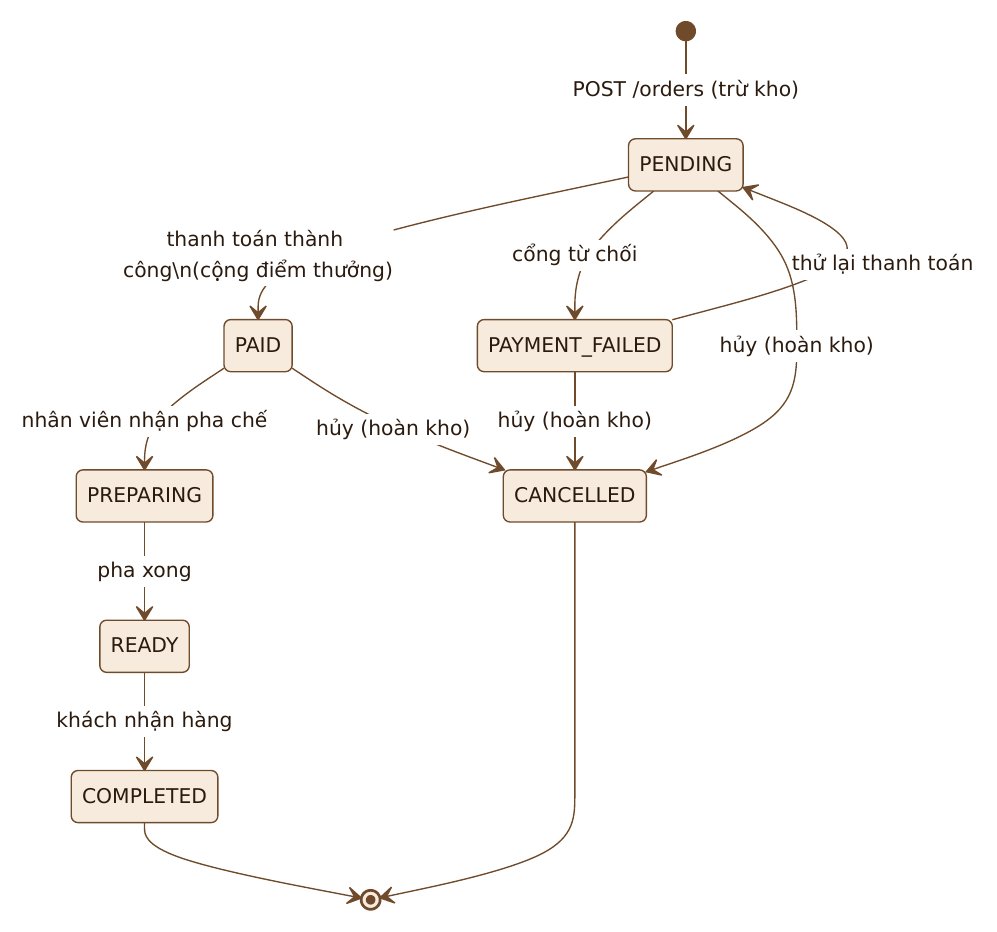
\includegraphics[width=0.47\textwidth,height=0.30\textheight,keepaspectratio]{img/a1/state-order.png}}\hspace{2mm}
\fbox{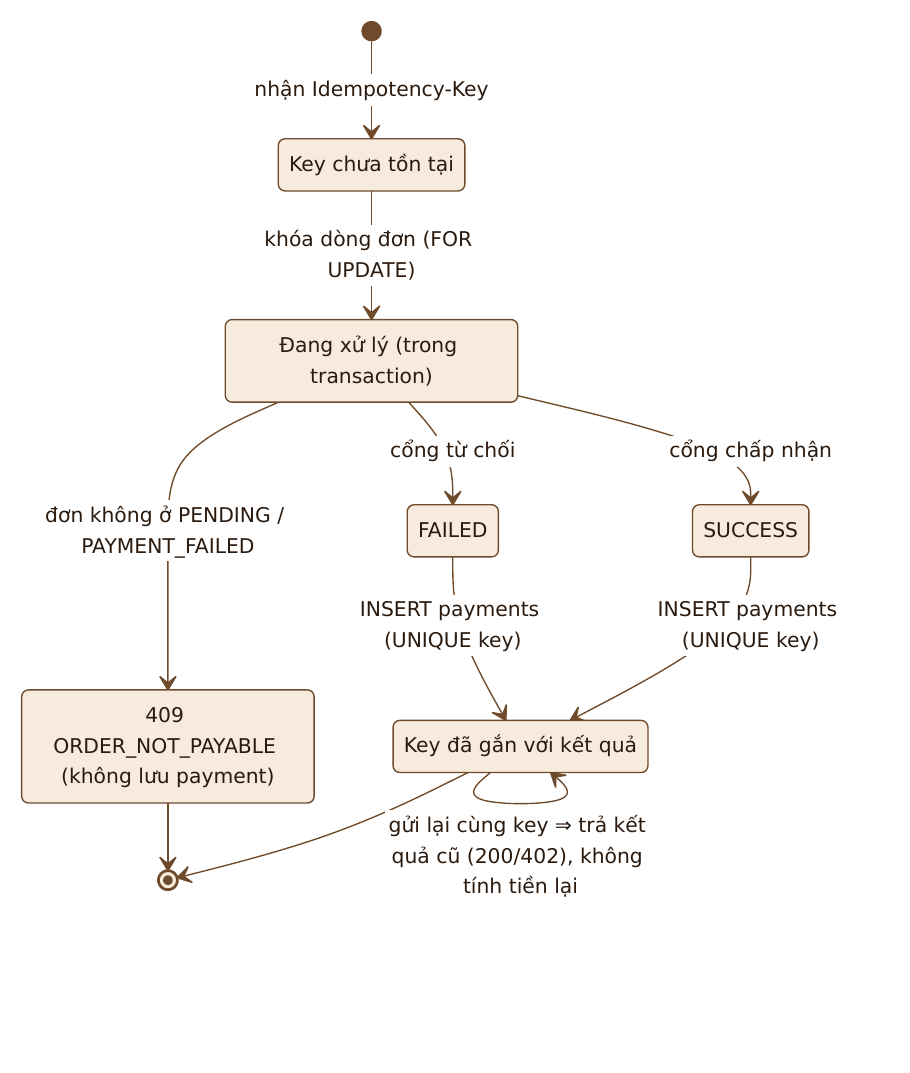
\includegraphics[width=0.47\textwidth,height=0.30\textheight,keepaspectratio]{img/a1/state-payment.png}}\hspace{2mm}
\end{center}\vspace{-2mm}
\qa{90}{\lvA}{State machine diagram mô tả gì?}{Vòng đời của MỘT đối tượng: các trạng thái và sự kiện/điều kiện làm nó chuyển trạng thái. Nhãn chuyển: sự kiện [guard] / hành động.}
\qa{91}{\lvA}{Đơn hàng có những trạng thái nào?}{7 trạng thái: PENDING, PAID, PREPARING, READY, COMPLETED, PAYMENT\_FAILED, CANCELLED. COMPLETED và CANCELLED là trạng thái kết thúc.}
\qa{92}{\lvA}{Các chuyển tiếp hợp lệ?}{PENDING $\rightarrow$ PAID, PAYMENT\_FAILED, CANCELLED; PAYMENT\_FAILED $\rightarrow$ PENDING, CANCELLED; PAID $\rightarrow$ PREPARING, CANCELLED; PREPARING $\rightarrow$ READY; READY $\rightarrow$ COMPLETED. Tổng 9 cặp hợp lệ trên 49 cặp (7$\times$7); 40 cặp còn lại bị chặn.}
\qa{93}{\lvA}{Chuyển trạng thái sai thì sao? Code nằm ở đâu?}{Hàm assertTransition trong apps/api/src/orders/order-status.ts ném 409 INVALID\_TRANSITION. Unit test UT-01..04 kiểm tra đủ 49 cặp.}
\qa{94}{\lvB}{Hai request đồng thời cùng chuyển một đơn thì sao?}{Câu UPDATE có điều kiện WHERE id = ? AND status = \textless{}trạng thái hiện tại\textgreater{}: chỉ request đầu tiên đổi được dòng, request sau thấy 0 dòng bị ảnh hưởng và bị từ chối.}
\qa{95}{\lvA}{Khách hủy được đơn ở trạng thái nào? Hủy thì có gì xảy ra?}{PENDING, PAYMENT\_FAILED, PAID (chưa pha chế). Hệ thống trả kho; nếu đã PAID thì thu hồi điểm (ghi LoyaltyTransaction REVOKE). PREPARING trở đi thì không hủy được (409).}
\qa{96}{\lvB}{Vì sao PAYMENT\_FAILED được quay lại PENDING?}{Để khách thử lại thanh toán trên CÙNG đơn (giữ nguyên giá và tồn kho đã giữ) thay vì tạo đơn mới làm giữ kho hai lần (lỗi D11 đã sửa).}
\qa{97}{\lvB}{State machine của Idempotency-Key gồm gì?}{Key mới $\rightarrow$ Đang xử lý (trong transaction, khóa dòng đơn) $\rightarrow$ SUCCESS hoặc FAILED (theo cổng) $\rightarrow$ Đã lưu (INSERT payments, UNIQUE key). Nhánh Từ chối khi đơn không thanh toán được (409, không lưu). Gửi lại key ở trạng thái Đã lưu thì trả kết quả cũ.}
\qa{98}{\lvB}{Ai được chuyển PREPARING, READY, COMPLETED?}{Chỉ nhân viên (role STAFF) qua PATCH /orders/:id/status, bảo vệ bằng RolesGuard; khách gọi nhận 403. Nhân viên không được đặt PAID bằng tay (400) vì PAID chỉ do thanh toán sinh ra.}
\section{Kiến trúc hệ thống}
\noindent\textit{Component, package, deployment (A1), C4, phân lớp, ADR, deployment production (A2).} \hfill \small(12 câu)\normalsize\par\medskip
\begin{center}
\fbox{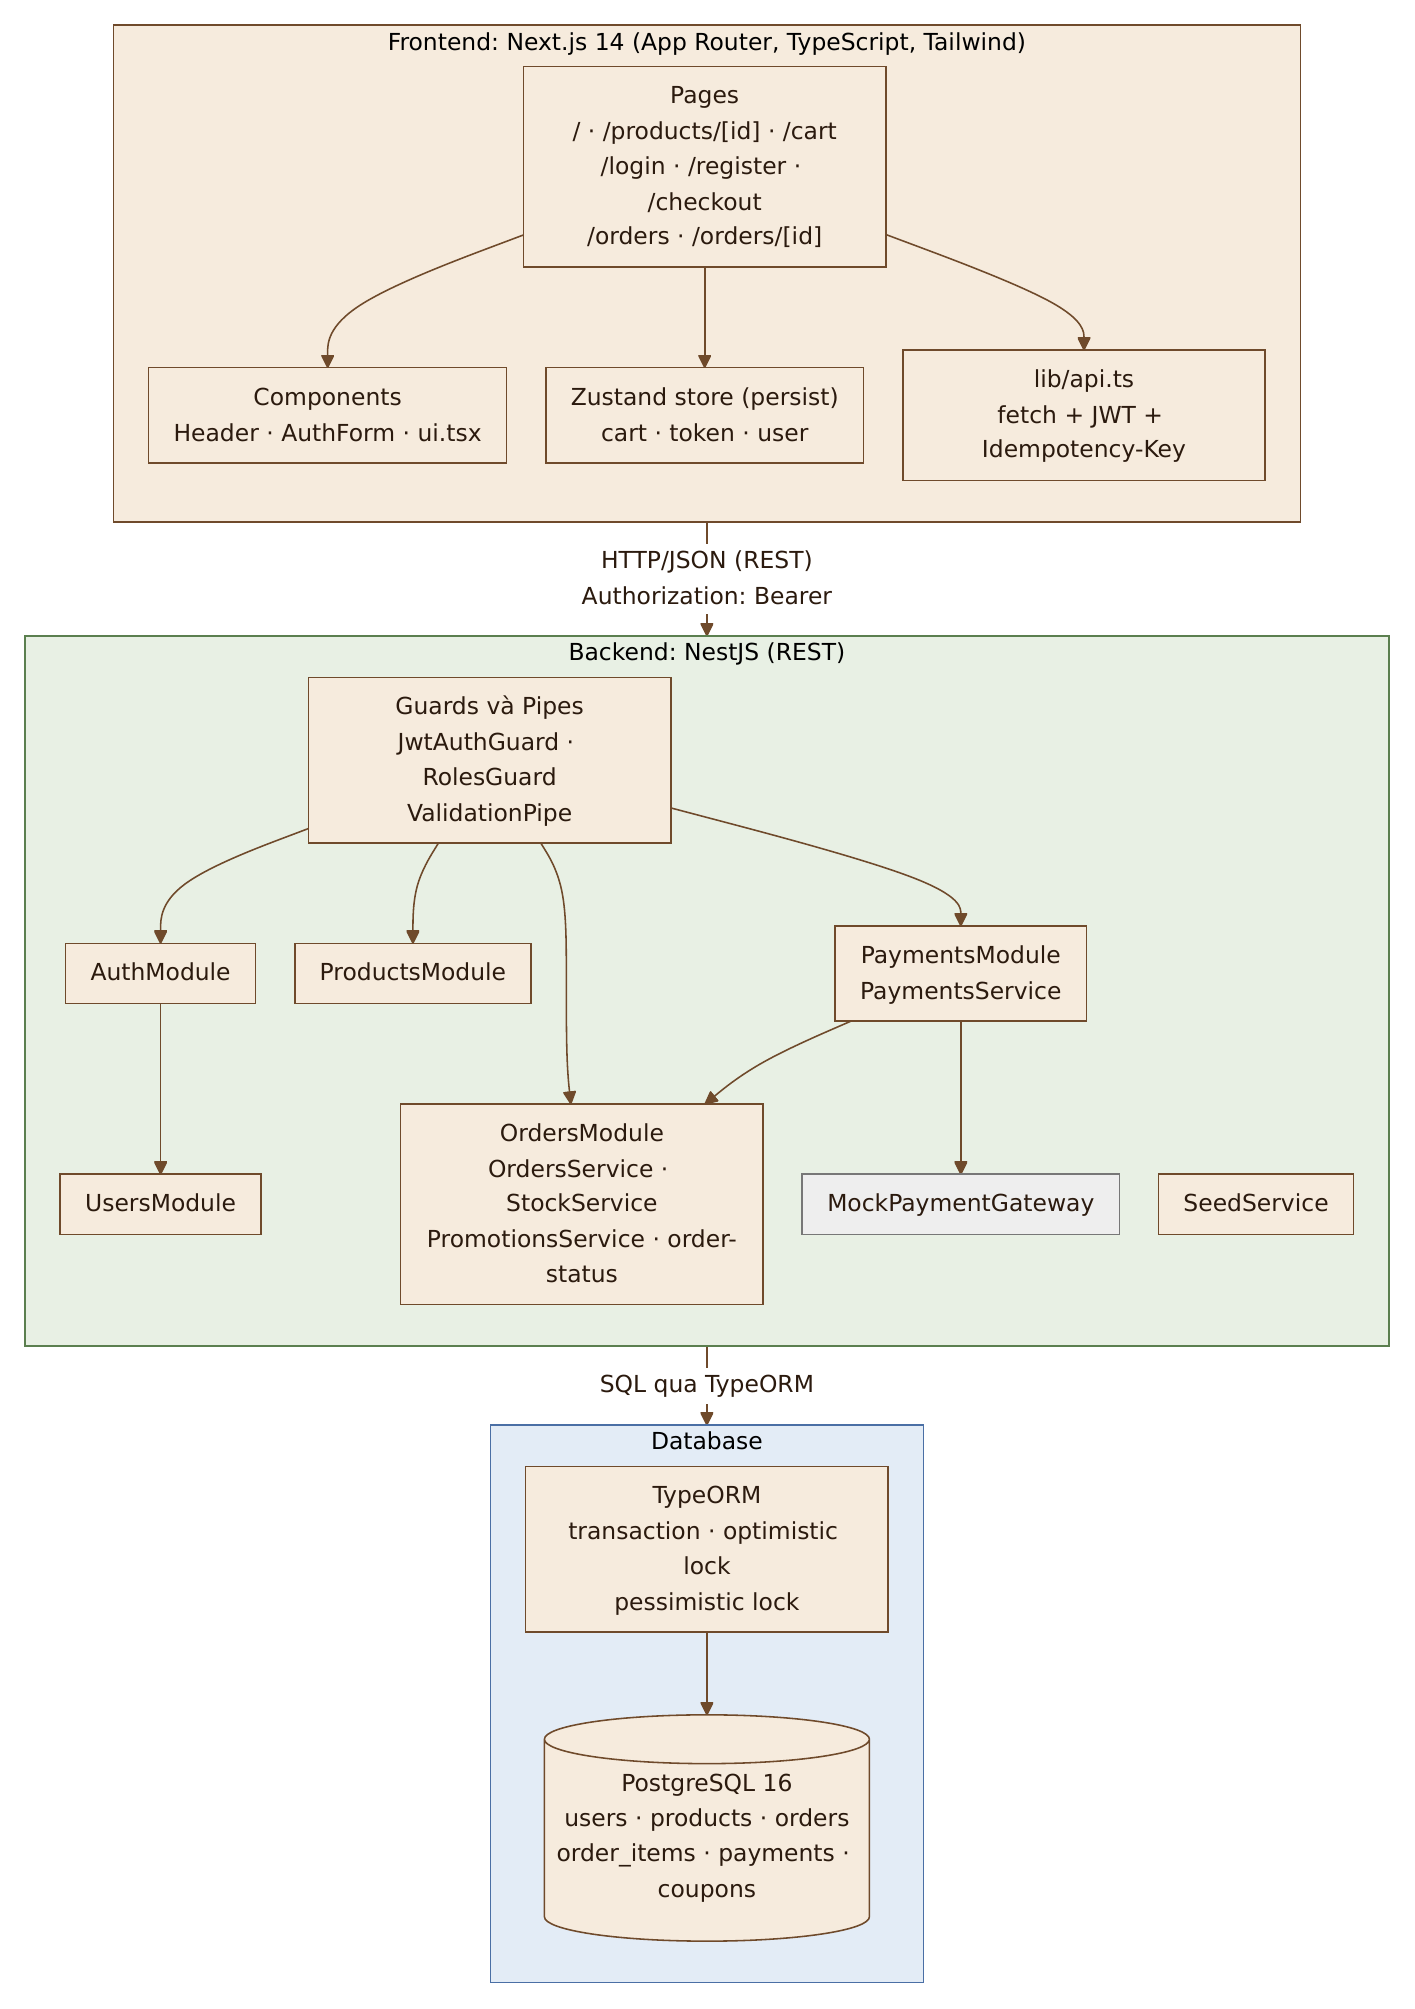
\includegraphics[width=0.31\textwidth,height=0.30\textheight,keepaspectratio]{img/a1/component.png}}\hspace{2mm}
\fbox{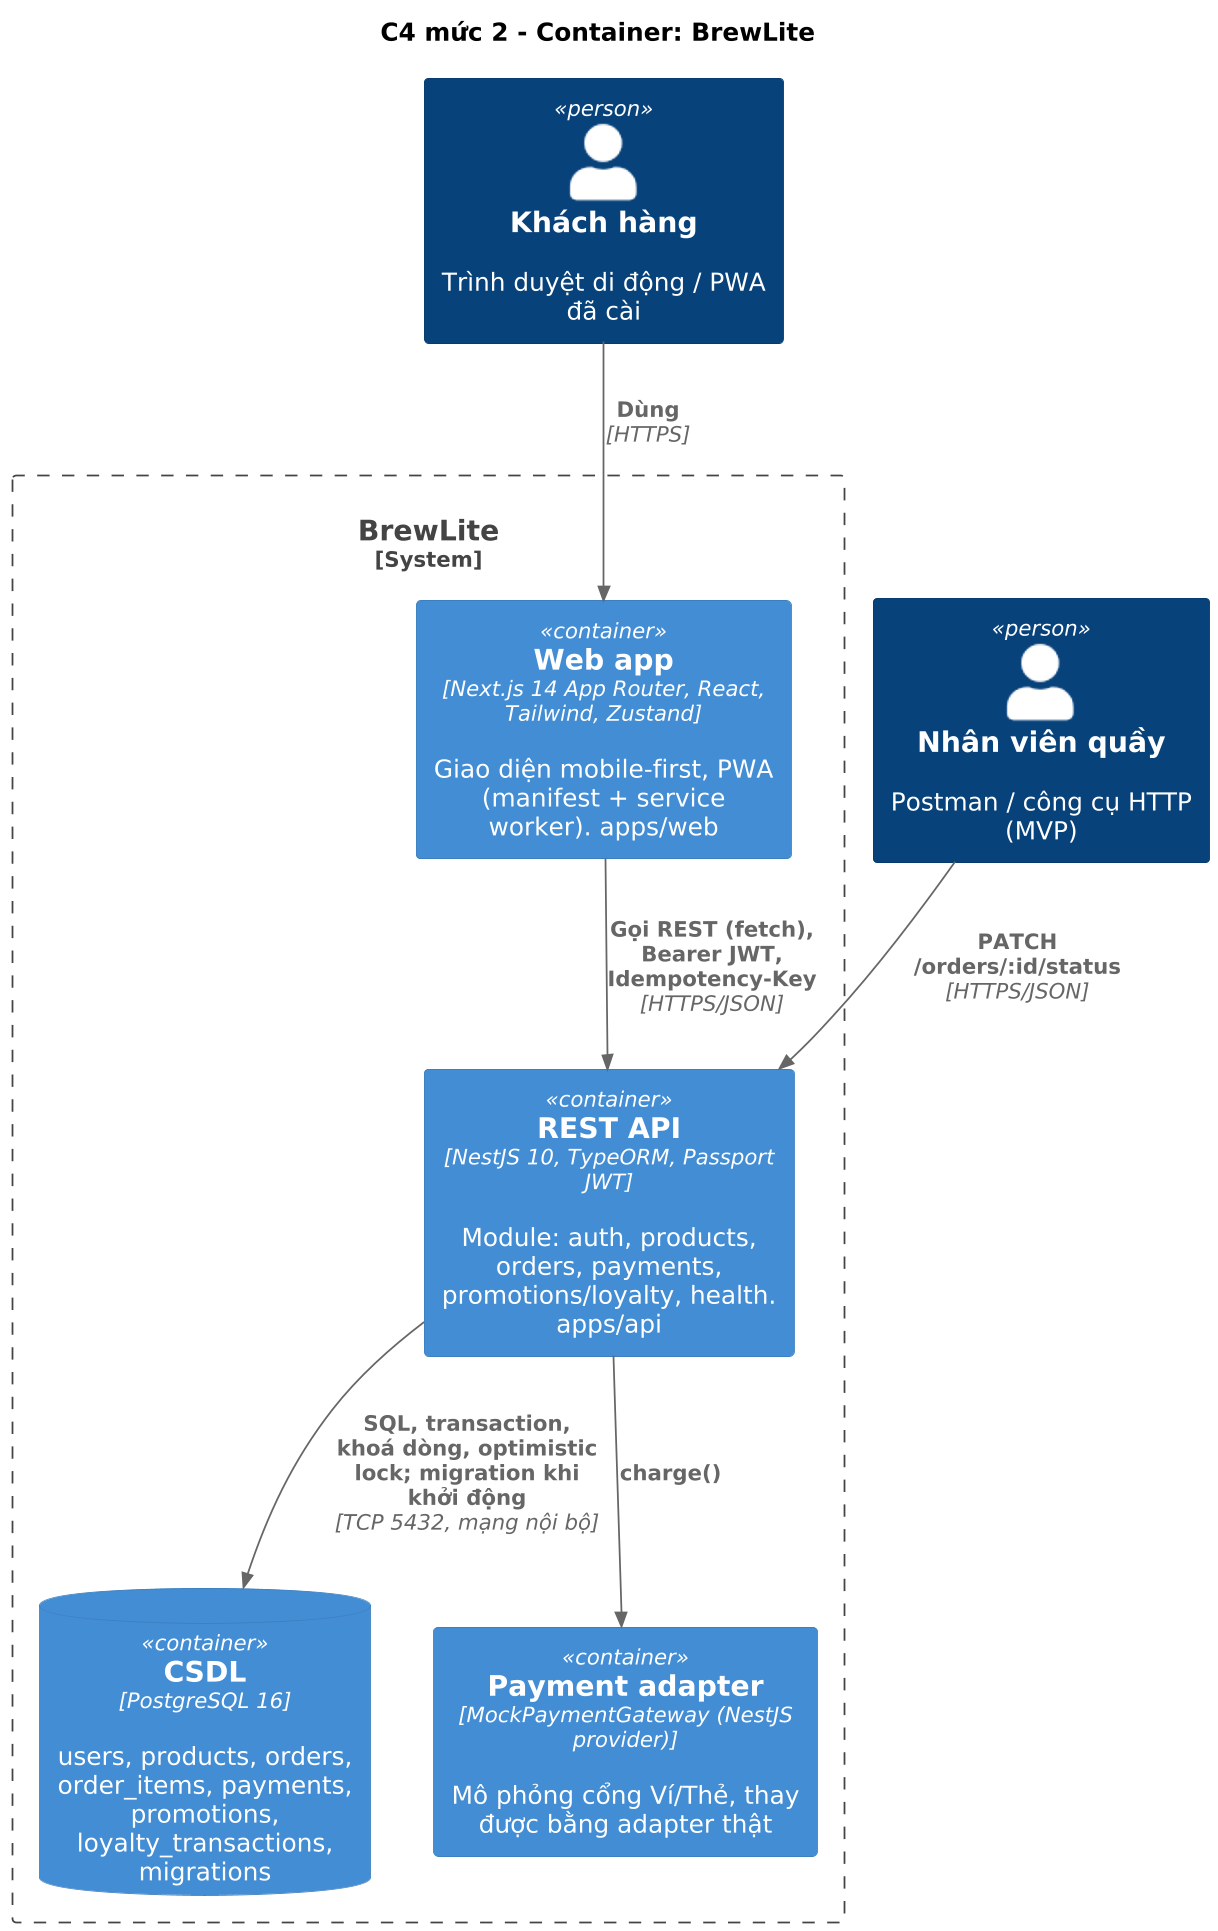
\includegraphics[width=0.31\textwidth,height=0.30\textheight,keepaspectratio]{img/a2/c4-container.png}}\hspace{2mm}
\fbox{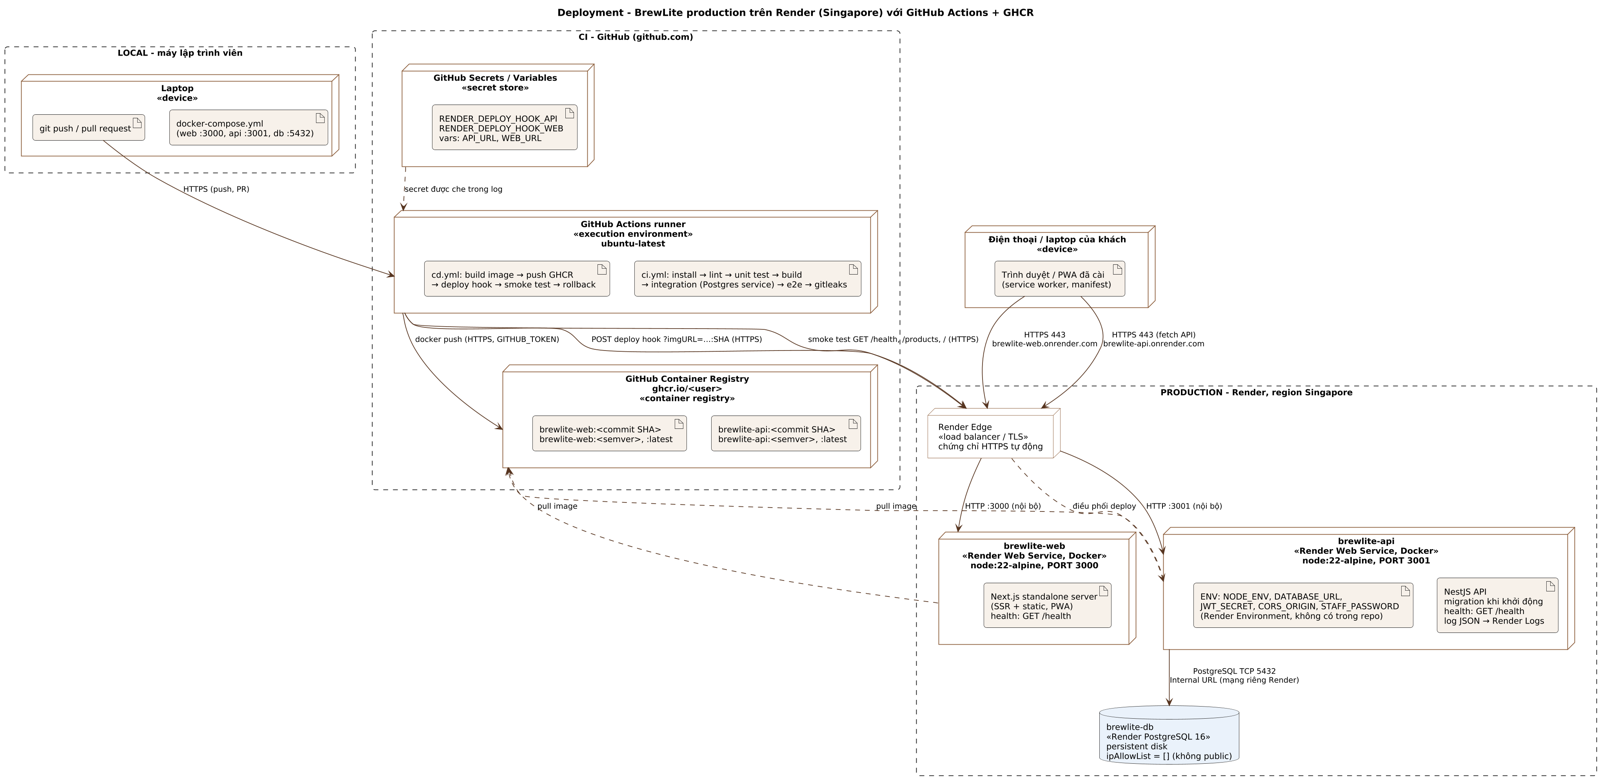
\includegraphics[width=0.31\textwidth,height=0.30\textheight,keepaspectratio]{img/a2/deployment-production.png}}\hspace{2mm}
\end{center}\vspace{-2mm}
\qa{99}{\lvA}{Kiến trúc tổng thể của BrewLite?}{Ba thành phần: Web app Next.js 14 (mobile-first, PWA) gọi REST API NestJS 10 qua HTTPS/JSON với Bearer JWT; API dùng TypeORM truy cập PostgreSQL 16. Payment adapter MockPaymentGateway chạy trong API. Đóng gói bằng Docker, chạy local bằng docker compose, production trên Render.}
\qa{100}{\lvA}{Mô hình C4 gồm những mức nào? Đồ án vẽ mức nào?}{Context (hệ thống và người dùng, hệ thống ngoài), Container (ứng dụng, CSDL chạy riêng), Component (thành phần trong container), Code. Đồ án vẽ mức 1 và 2; mức 3 thể hiện bằng cấu trúc module NestJS.}
\qa{101}{\lvA}{Backend chia lớp thế nào?}{Presentation: controller, DTO + class-validator, guard (không chứa nghiệp vụ). Application/Domain: service và hàm thuần (unitPrice, computeDiscount, assertTransition). Infrastructure: entity, migration, MockPaymentGateway, PostgreSQL.}
\qa{102}{\lvB}{NestJS module gồm những gì? Đồ án có module nào?}{Module gom controller, provider (service) và import/export. Đồ án: auth, users, products, orders, payments, promotions, loyalty, seed, health. Module chỉ dùng nhau qua service được export.}
\qa{103}{\lvA}{Component, package, deployment diagram khác nhau thế nào?}{Component: các thành phần phần mềm và giao diện giữa chúng (có gì). Package: cách nhóm mã nguồn và phụ thuộc giữa các gói (nhóm ra sao). Deployment: phần mềm chạy trên node nào, cổng, kết nối (chạy ở đâu).}
\qa{104}{\lvA}{ADR là gì? Đồ án có những ADR nào?}{Architecture Decision Record: ghi một quyết định kiến trúc gồm bối cảnh, phương án, quyết định, hệ quả. 7 ADR: 001 monorepo; 002 modular monolith; 003 PostgreSQL + TypeORM + migration; 004 migration khi khởi động trong 1 transaction; 005 idempotency + khóa dòng + optimistic lock; 006 Render + GHCR + GitHub Actions; 007 JWT Bearer + bcrypt.}
\qa{105}{\lvB}{Vì sao chọn modular monolith thay vì microservices?}{Đặt đơn, trừ kho, thanh toán và cộng điểm cần một transaction ACID chung. Microservices cần saga/outbox, nhiều container, chi phí vận hành cao, không hợp với nhóm một người và lưu lượng nhỏ. Ranh giới module vẫn cho phép tách sau này (ví dụ tách payment).}
\qa{106}{\lvA}{Deployment diagram production có những gì?}{3 vùng: LOCAL (laptop, docker compose), CI (GitHub Actions runner, GitHub Secrets, GHCR), PRODUCTION (Render Singapore: Render Edge HTTPS, brewlite-web cổng 3000, brewlite-api cổng 3001, brewlite-db PostgreSQL 16 có persistent disk, không public). Người dùng $\rightarrow$ HTTPS 443 $\rightarrow$ Edge $\rightarrow$ web/api; api $\rightarrow$ db qua Internal URL 5432.}
\qa{107}{\lvB}{Làm sao chứng minh deployment diagram truy vết được tới mã nguồn?}{Bảng cuối architecture.md: brewlite-web $\leftrightarrow$ apps/web + Dockerfile + render.yaml; brewlite-api $\leftrightarrow$ apps/api; brewlite-db $\leftrightarrow$ apps/api/src/database + render.yaml databases; GHCR $\leftrightarrow$ job image trong cd.yml; secret $\leftrightarrow$ .env.example, render.yaml envVars, GitHub Secrets; health $\leftrightarrow$ health.controller.ts.}
\qa{108}{\lvA}{Docker Compose local gồm những gì?}{3 dịch vụ: db (postgres:16-alpine, cổng 5432, healthcheck pg\_isready, volume brewlite-db), api (NestJS 3001, chờ db khỏe, chạy migration + seed), web (Next.js 3000, chờ api khỏe; NEXT\_PUBLIC\_API\_URL nhúng lúc build).}
\qa{109}{\lvB}{Vì sao NEXT\_PUBLIC\_API\_URL đổi thì phải build lại web?}{Next.js thay biến NEXT\_PUBLIC\_* vào mã JavaScript lúc build để trình duyệt dùng được. Đổi giá trị lúc chạy không có tác dụng, phải build lại image.}
\qa{110}{\lvA}{Sitemap (A1) có những trang nào?}{/ Menu, /products/:id, /cart, /login, /register, /checkout, /orders, /orders/:id. Chưa đăng nhập bấm Thanh toán $\rightarrow$ /login?next=/checkout; thanh toán thành công $\rightarrow$ /orders/:id; thất bại $\rightarrow$ ở lại /checkout.}
\section{Luồng nghiệp vụ và Task 10}
\noindent\textit{Giá, khuyến mãi, điểm, idempotency, tồn kho đồng thời, mã lỗi HTTP.} \hfill \small(13 câu)\normalsize\par\medskip
\qa{111}{\lvA}{Giá một ly tính thế nào? Ví dụ.}{Giá gốc (size M) + chênh lệch size (S $-$5.000, M 0, L +7.000) + tổng topping (Trân châu 5.000, Kem 7.000, Thạch dừa 5.000, Espresso shot 10.000; mỗi loại tính một lần). Cappuccino 45.000 size L + Trân châu = 45.000 + 7.000 + 5.000 = 57.000đ.}
\qa{112}{\lvA}{Vì sao giá phải tính ở server?}{Client có thể bị sửa (DevTools, gọi API trực tiếp). Server tính lại từ bảng giá gốc + size + topping nên không ai gửi giá thấp để gian lận. Frontend chỉ hiển thị để tiện.}
\qa{113}{\lvA}{Hai mã giảm giá hoạt động thế nào?}{BREW10: giảm 10\%, tối đa 20.000đ, không yêu cầu đơn tối thiểu. WELCOME20: giảm 20\% cho đơn từ 100.000đ, tối đa 50.000đ. Giảm làm tròn xuống. Mã không phân biệt hoa thường; sai, hết hạn hoặc chưa đủ tối thiểu trả 400.}
\qa{114}{\lvA}{Điểm thưởng tính và lưu thế nào?}{$\lfloor$tổng thanh toán / 10.000$\rfloor$, cộng đúng một lần khi đơn chuyển PAID (cờ pointsAwarded + UNIQUE(orderId, type)). Hủy đơn đã PAID thì thu hồi đúng số điểm. Mỗi lần ghi một dòng loyalty\_transactions (EARN/REVOKE); users.loyaltyPoints là số dư; GET /loyalty/me trả số dư và lịch sử.}
\qa{115}{\lvA}{Idempotent là gì? Vì sao thanh toán cần idempotent?}{Gửi một yêu cầu nhiều lần cho kết quả như gửi một lần. Khách có thể bấm nhiều lần hoặc mạng rớt rồi trình duyệt gửi lại; nếu không idempotent sẽ trừ tiền hai lần.}
\qa{116}{\lvB}{Idempotency được hiện thực bằng những cơ chế nào?}{Header Idempotency-Key bắt buộc ở POST /payments (thiếu 400); cột idempotencyKey UNIQUE; tìm key trước khi xử lý (có thì trả kết quả cũ, 200 + Idempotent-Replayed: true); khóa dòng đơn SELECT ... FOR UPDATE rồi kiểm tra lại key; key dùng cho đơn khác trả 409. POST /orders cũng hỗ trợ key (UNIQUE userId + key), 5 request đồng thời chỉ tạo 1 đơn.}
\qa{117}{\lvB}{Chống bán vượt tồn kho thế nào?}{Optimistic locking: UPDATE products SET stock = stock $-$ qty, version = version + 1 WHERE id = ? AND version = ? AND stock \textgreater{}= qty. 0 dòng $\rightarrow$ đọc lại, thử lại tối đa 8 lần; sắp xếp id để thứ tự khóa nhất quán; thiếu hàng $\rightarrow$ 409 OUT\_OF\_STOCK và rollback cả đơn. CHECK stock \textgreater{}= 0 là lớp bảo vệ cuối. Test: 12 khách tranh 5 ly ra đúng 5 đơn.}
\qa{118}{\lvB}{Optimistic và pessimistic locking khác nhau ra sao?}{Pessimistic khóa dữ liệu trước khi sửa, người khác phải chờ (SELECT ... FOR UPDATE). Optimistic không khóa, kiểm tra xung đột lúc ghi bằng version, xung đột thì thử lại. Pessimistic hợp tranh chấp cao hoặc thao tác dài; optimistic hợp xung đột thấp, thao tác ngắn, cần thông lượng.}
\qa{119}{\lvC}{Vì sao sắp xếp id sản phẩm trước khi trừ kho?}{Để mọi giao dịch truy cập dòng theo cùng một thứ tự, tránh hai giao dịch giữ dòng theo thứ tự ngược nhau gây xung đột/deadlock.}
\qa{120}{\lvA}{Mã HTTP trong đồ án?}{201 tạo thành công; 200 phát lại idempotent; 400 dữ liệu sai/thiếu key/mã giảm giá sai; 401 chưa đăng nhập/token sai; 402 thanh toán thất bại; 403 không đủ quyền; 404 không tìm thấy; 409 xung đột (INVALID\_TRANSITION, OUT\_OF\_STOCK, ORDER\_NOT\_PAYABLE, key dùng cho đơn khác, email trùng).}
\qa{121}{\lvA}{3 tiêu chí chấm của Task 10 (A1) và cách chứng minh?}{(a) Chặn chuyển trạng thái sai $\rightarrow$ UT-01..04 (49 cặp) và INT-T11. (b) Gửi hai lần cùng Idempotency-Key chỉ tạo một đơn $\rightarrow$ INT-T14, T15 (5 request đồng thời). (c) Đặt đồng thời không vượt tồn kho $\rightarrow$ INT-T18..T20 (12 khách/5 ly, 30 khách/10 ly).}
\qa{122}{\lvA}{Thanh toán thất bại thì dữ liệu ra sao?}{Đơn chuyển PAYMENT\_FAILED, lưu payment FAILED cùng key và lý do, COMMIT, trả 402. Kho vẫn giữ cho đơn, giỏ hàng còn nguyên, không cộng điểm. Khách thử lại bằng key mới: đơn về PENDING rồi thanh toán.}
\qa{123}{\lvC}{Nếu cổng thanh toán trừ tiền thành công nhưng server sập trước COMMIT thì sao?}{Đây là giới hạn của bản mô phỏng: transaction rollback nên đơn vẫn PENDING dù tiền đã trừ. Với cổng thật cần gửi Idempotency-Key sang cổng, dùng webhook từ cổng và job đối soát để cập nhật đơn theo kết quả thực tế (outbox/reconciliation). Đã ghi trong hướng phát triển.}
\section{Bảo mật và xác thực}
\noindent\textit{JWT, bcrypt, phân quyền, validate, CORS, secret.} \hfill \small(9 câu)\normalsize\par\medskip
\qa{124}{\lvA}{JWT là gì? Cấu trúc thế nào?}{JSON Web Token gồm 3 phần header.payload.signature mã hóa base64url. Server ký bằng JWT\_SECRET (HS256); client gửi trong header Authorization: Bearer \textless{}token\textgreater{}; server kiểm tra chữ ký và hạn (1 ngày) mà không cần lưu phiên.}
\qa{125}{\lvB}{Payload JWT có bị mã hóa không? Có nên để mật khẩu trong đó?}{Không, chỉ mã hóa base64, ai cũng đọc được; chữ ký chỉ chống sửa. Không đặt dữ liệu nhạy cảm, chỉ id, email, role.}
\qa{126}{\lvA}{Vì sao băm mật khẩu bằng bcrypt mà không dùng MD5/SHA?}{bcrypt có salt riêng mỗi mật khẩu và cố ý chậm (cost 10, khoảng 68 ms) để chống dò mật khẩu hàng loạt và rainbow table. MD5/SHA quá nhanh nên dễ bị brute-force.}
\qa{127}{\lvA}{Phân quyền được thực hiện thế nào?}{JwtAuthGuard bảo vệ route cần đăng nhập; RolesGuard + @Roles('STAFF') cho API nhân viên; service kiểm tra khách chỉ xem/hủy đơn của chính mình (403).}
\qa{128}{\lvA}{Validate đầu vào ở backend thế nào?}{ValidationPipe toàn cục với whitelist (bỏ trường lạ) và forbidNonWhitelisted (gửi trường lạ thì 400), DTO dùng class-validator: email hợp lệ, mật khẩu $\ge$ 6 ký tự, size thuộc S/M/L, qty 1–20, method thuộc WALLET/CARD.}
\qa{129}{\lvB}{CORS là gì? Lỗi G07 là gì?}{CORS là cơ chế trình duyệt chỉ cho trang ở origin khác gọi API khi server cho phép. Lỗi G07: không đặt CORS\_ORIGIN thì API nhận mọi nguồn; đã sửa để mặc định chỉ http://localhost:3000 và production đặt đúng URL web.}
\qa{130}{\lvB}{Secret được quản lý thế nào ở production?}{.env không commit; .env.example chỉ có giá trị giả; JWT\_SECRET do Render sinh; deploy hook trong GitHub Secrets (environment production), GitHub che trong log; CSDL không public; gitleaks quét lịch sử git mỗi PR; production thiếu biến hoặc JWT\_SECRET \textless{} 32 ký tự thì app không khởi động.}
\qa{131}{\lvC}{Lưu JWT trong localStorage có rủi ro gì? Cải tiến thế nào?}{Nếu trang bị XSS, script độc đọc được token. Giảm thiểu: React tự escape, không dùng dangerouslySetInnerHTML, token hết hạn 1 ngày. Cải tiến: cookie HttpOnly + SameSite và refresh token xoay vòng.}
\qa{132}{\lvA}{Lỗi C07 là gì?}{Token hết hạn khiến giao diện kẹt (gọi API liên tục lỗi). Sửa: nhận 401 thì tự đăng xuất và chuyển về /login, giỏ hàng giữ nguyên.}
\section{Kiểm thử}
\noindent\textit{Unit, integration, component, E2E, bộ 55 kịch bản giao diện, 6 lỗi đã sửa.} \hfill \small(10 câu)\normalsize\par\medskip
\qa{133}{\lvA}{Các mức kiểm thử trong đồ án?}{Unit test (hàm thuần: state machine, giá, khuyến mãi, cấu hình) – 15; integration test API với PostgreSQL thật – 27; test component web Vitest – 7; E2E Playwright luồng menu $\rightarrow$ xác nhận – 1; kiểm thử giao diện thủ công/tự động 55 kịch bản, 224 điểm kiểm tra (A1). Tổng test tự động A2: 50.}
\qa{134}{\lvA}{Unit test khác integration test và E2E thế nào?}{Unit: kiểm tra một đơn vị nhỏ độc lập, nhanh, không cần CSDL. Integration: kiểm tra nhiều thành phần chạy cùng nhau (HTTP + service + PostgreSQL thật). E2E: kiểm tra như người dùng thật trên trình duyệt, đi qua toàn bộ hệ thống.}
\qa{135}{\lvB}{Kim tự tháp kiểm thử là gì?}{Nhiều unit test ở đáy (rẻ, nhanh), ít integration hơn ở giữa, rất ít E2E ở đỉnh (chậm, dễ vỡ). Đồ án theo đúng tỉ lệ đó: 15 unit + 27 integration + 7 component, 1 E2E.}
\qa{136}{\lvB}{Integration test dùng CSDL nào? Có ảnh hưởng dữ liệu thật không?}{CSDL riêng brewlite\_test (TEST\_DATABASE\_URL). Mỗi lần chạy xóa schema (dropSchema) rồi chạy lại toàn bộ migration, nên không ảnh hưởng dữ liệu thật và đồng thời chứng minh migration tái tạo được CSDL.}
\qa{137}{\lvB}{Test đồng thời tồn kho viết thế nào?}{Tạo sản phẩm còn 5 ly, bắn 12 request POST /orders song song bằng Promise.all, khẳng định đúng 5 request 201, 7 request 409 và stock cuối = 0, không âm.}
\qa{138}{\lvA}{E2E-T01 đi qua những bước nào?}{Mở / trên khung Pixel 7 $\rightarrow$ bấm Cappuccino $\rightarrow$ chọn size L $\rightarrow$ Thêm vào giỏ $\rightarrow$ /cart có 1 dòng $\rightarrow$ Thanh toán $\rightarrow$ bị chuyển /login $\rightarrow$ Đăng ký tài khoản mới $\rightarrow$ về /checkout $\rightarrow$ chọn Ví điện tử $\rightarrow$ Xác nhận thanh toán $\rightarrow$ /orders/:id thấy 'Đã thanh toán' $\rightarrow$ /orders thấy đơn.}
\qa{139}{\lvB}{Test component Menu kiểm tra gì?}{FE-T01: trạng thái loading (role status), danh sách có giá VND và nhãn Hết hàng, link tới /products/:id, trạng thái 'Menu đang trống', lỗi kết nối có nút Thử lại và gọi lại API. Dùng vi.mock để giả lập api.}
\qa{140}{\lvB}{6 lỗi nghiệp vụ tìm được là gì?}{F04 (cao) giá đổi khi khách đang xem giỏ mà vẫn thanh toán $\rightarrow$ so tổng, hỏi lại. D11 thanh toán lỗi rồi tải lại tạo đơn thứ hai $\rightarrow$ dùng lại đơn cũ. D12 thanh toán lại từ chi tiết đơn nhưng giỏ không xóa $\rightarrow$ xóa đúng món. E06 hủy đơn PAID không thu hồi điểm $\rightarrow$ revokePoints. C07 token hết hạn kẹt giao diện $\rightarrow$ tự đăng xuất. G07 CORS nhận mọi nguồn $\rightarrow$ mặc định localhost:3000.}
\qa{141}{\lvB}{Hộp đen và hộp trắng khác nhau thế nào? Đồ án dùng loại nào?}{Hộp đen: thiết kế test từ đặc tả, không nhìn code (E2E, kịch bản giao diện, phần lớn integration theo API). Hộp trắng: dựa trên cấu trúc code, nhánh, đường đi (unit test state machine phủ đủ 49 cặp). Đồ án dùng cả hai.}
\qa{142}{\lvB}{Phân vùng tương đương và giá trị biên áp dụng thế nào?}{Ví dụ qty hợp lệ 1–20: phân vùng \textless{} 1, 1–20, \textgreater{} 20; giá trị biên 0, 1, 20, 21. WELCOME20: đơn 99.999 (không áp), 100.000 (áp). Mật khẩu 5 và 6 ký tự.}
\section{DevOps: Docker, migration, CI/CD, triển khai}
\noindent\textit{Task 4.4, 5.2, 5.3, 5.4 của A2.} \hfill \small(16 câu)\normalsize\par\medskip
\begin{center}
\fbox{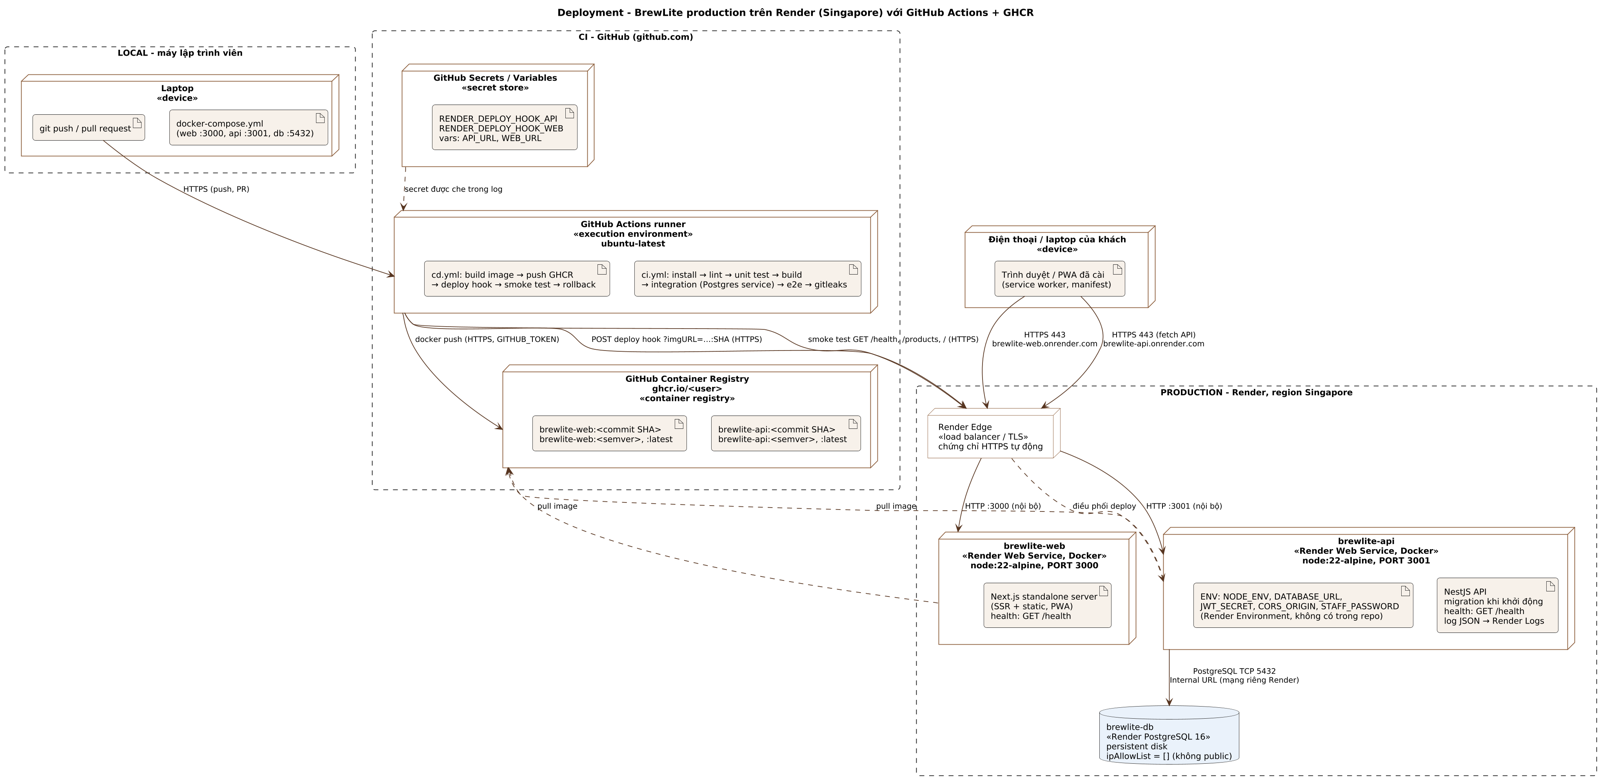
\includegraphics[width=0.62\textwidth,height=0.30\textheight,keepaspectratio]{img/a2/deployment-production.png}}\hspace{2mm}
\end{center}\vspace{-2mm}
\qa{143}{\lvA}{CI và CD khác nhau thế nào?}{CI (Continuous Integration): mỗi thay đổi được tích hợp và kiểm tra tự động (lint, test, build) để phát hiện lỗi sớm. CD: Continuous Delivery tự động đóng gói và luôn sẵn sàng triển khai; Continuous Deployment tự động triển khai lên production khi qua kiểm tra.}
\qa{144}{\lvA}{Pipeline CI của em gồm những bước nào? Chạy khi nào?}{Chạy khi mở/cập nhật PR vào main. Job quality (matrix api, web): Install $\rightarrow$ Lint $\rightarrow$ Unit Test $\rightarrow$ Build. Sau đó integration test với PostgreSQL service, E2E Playwright, gitleaks quét secret.}
\qa{145}{\lvA}{Làm sao PR không merge được khi CI lỗi?}{Bật branch protection cho main: Require a pull request before merging + Require status checks to pass (chọn các job CI). Check đỏ thì nút Merge bị khóa.}
\qa{146}{\lvA}{Pipeline CD có những bước nào?}{Push/tag $\rightarrow$ quality gate (gọi lại ci.yml) $\rightarrow$ build Docker image $\rightarrow$ tag commit SHA (và semver khi có tag) $\rightarrow$ push GHCR $\rightarrow$ gọi deploy hook Render cho API (migration chạy khi container khởi động) $\rightarrow$ chờ /health báo đúng SHA $\rightarrow$ deploy web $\rightarrow$ smoke test $\rightarrow$ lỗi thì rollback về SHA trước và dừng pipeline với lỗi $\rightarrow$ tag thì tạo GitHub Release.}
\qa{147}{\lvB}{Vì sao tag image bằng commit SHA?}{SHA là duy nhất và bất biến, biết chính xác code nào đang chạy, rollback chỉ là deploy lại một image cũ. latest thì thay đổi theo thời gian nên không truy vết được.}
\qa{148}{\lvB}{Migration chạy ở đâu và an toàn thế nào?}{Khi container API mới khởi động, mọi migration chưa chạy nằm trong một transaction. Lỗi thì rollback, app dừng, health check không đạt, Render không chuyển traffic, bản cũ vẫn chạy và pipeline rollback. Migration viết tương thích ngược (expand/contract) để rollback image vẫn chạy.}
\qa{149}{\lvA}{Smoke test kiểm tra gì?}{API /health trả status ok, db up và version đúng SHA vừa deploy; GET /products có dữ liệu; web /health đúng SHA; trang Menu trả 200 có chữ BrewLite; manifest PWA đúng. Có thử lại vì dịch vụ cần thời gian kéo image và khởi động.}
\qa{150}{\lvA}{Rollback có những cách nào?}{Tự động trong pipeline khi deploy/smoke test lỗi (deploy lại SHA đọc được từ /health trước khi deploy). Bằng tay: Actions $\rightarrow$ CD $\rightarrow$ Run workflow với rollback\_to = \textless{}SHA\textgreater{}. Trên Render: Events $\rightarrow$ chọn bản trước $\rightarrow$ Rollback. Hoàn tác schema hiếm khi cần: migration:revert:prod.}
\qa{151}{\lvA}{Health check endpoint trả gì?}{API GET /health: \{status, db, migrations, version (commit SHA), uptime\}; 200 khi CSDL trả lời SELECT 1, 503 khi CSDL lỗi. Web GET /health: \{status, service, version\}. Render dùng làm health check; pipeline dùng để xác nhận đúng phiên bản.}
\qa{152}{\lvB}{Vì sao chọn Render và GHCR?}{Miễn phí, HTTPS tự động, chạy được Docker image, PostgreSQL có Internal URL, deploy hook nhận image theo SHA, hạ tầng khai báo bằng render.yaml. GHCR gắn liền GitHub, đăng nhập bằng GITHUB\_TOKEN. Hạn chế: gói miễn phí ngủ sau 15 phút, Postgres miễn phí hết hạn 30 ngày.}
\qa{153}{\lvB}{render.yaml dùng để làm gì?}{Blueprint – hạ tầng dưới dạng code: khai báo brewlite-db (Postgres 16, Singapore, ipAllowList rỗng), brewlite-api và brewlite-web (runtime image từ GHCR, healthCheckPath /health, autoDeploy false), biến môi trường (DATABASE\_URL lấy từ DB, JWT\_SECRET sinh tự động, CORS\_ORIGIN nhập tay).}
\qa{154}{\lvA}{Log được ghi thế nào?}{Middleware RequestLogger ghi một dòng mỗi request \{method, path, status, ms\}, JSON ở production, 5xx mức error, 4xx mức warn, bỏ qua /health 200, không ghi header, body, query. Xem trên Render Logs.}
\qa{155}{\lvA}{PWA là gì? Đồ án làm những gì cho PWA?}{Progressive Web App: web cài được lên màn hình chính, chạy như app, có khả năng ngoại tuyến. Đồ án có app/manifest.ts (name, short\_name, start\_url, display standalone, icon 192/512/maskable), service worker public/sw.js (trang network-first, tài nguyên tĩnh cache-first, không cache API), trang offline.html, đăng ký service worker chỉ ở production.}
\qa{156}{\lvB}{Vì sao service worker không cache API?}{Giá, tồn kho, trạng thái đơn phải luôn mới; cache API có thể khiến khách thấy giá cũ hoặc đơn sai trạng thái. Hơn nữa API ở origin khác nên service worker để mạng xử lý.}
\qa{157}{\lvB}{Dockerfile multi-stage là gì? Có lợi gì?}{Stage build cài devDependencies và build; stage chạy chỉ copy dist/node\_modules production. Image nhỏ hơn, ít bề mặt tấn công hơn. Container chạy bằng user node (không phải root) và có HEALTHCHECK.}
\qa{158}{\lvC}{Nếu Render đang ngủ lúc thầy mở link thì sao?}{Gói miễn phí ngủ sau 15 phút không có request, lần đầu mất khoảng 1 phút để khởi động. Em mở web và /health trước giờ chấm khoảng 2 phút; nếu đang chờ thì giải thích đây là đặc điểm gói miễn phí đã ghi trong rủi ro R-04.}
\section{Demo giao diện và chức năng}
\noindent\textit{Kịch bản demo và các yêu cầu thao tác thầy có thể đưa ra. Cột phải là kết quả em cần chỉ ra trên màn hình.} \hfill \small(14 câu)\normalsize\par\medskip
\begin{center}
\fbox{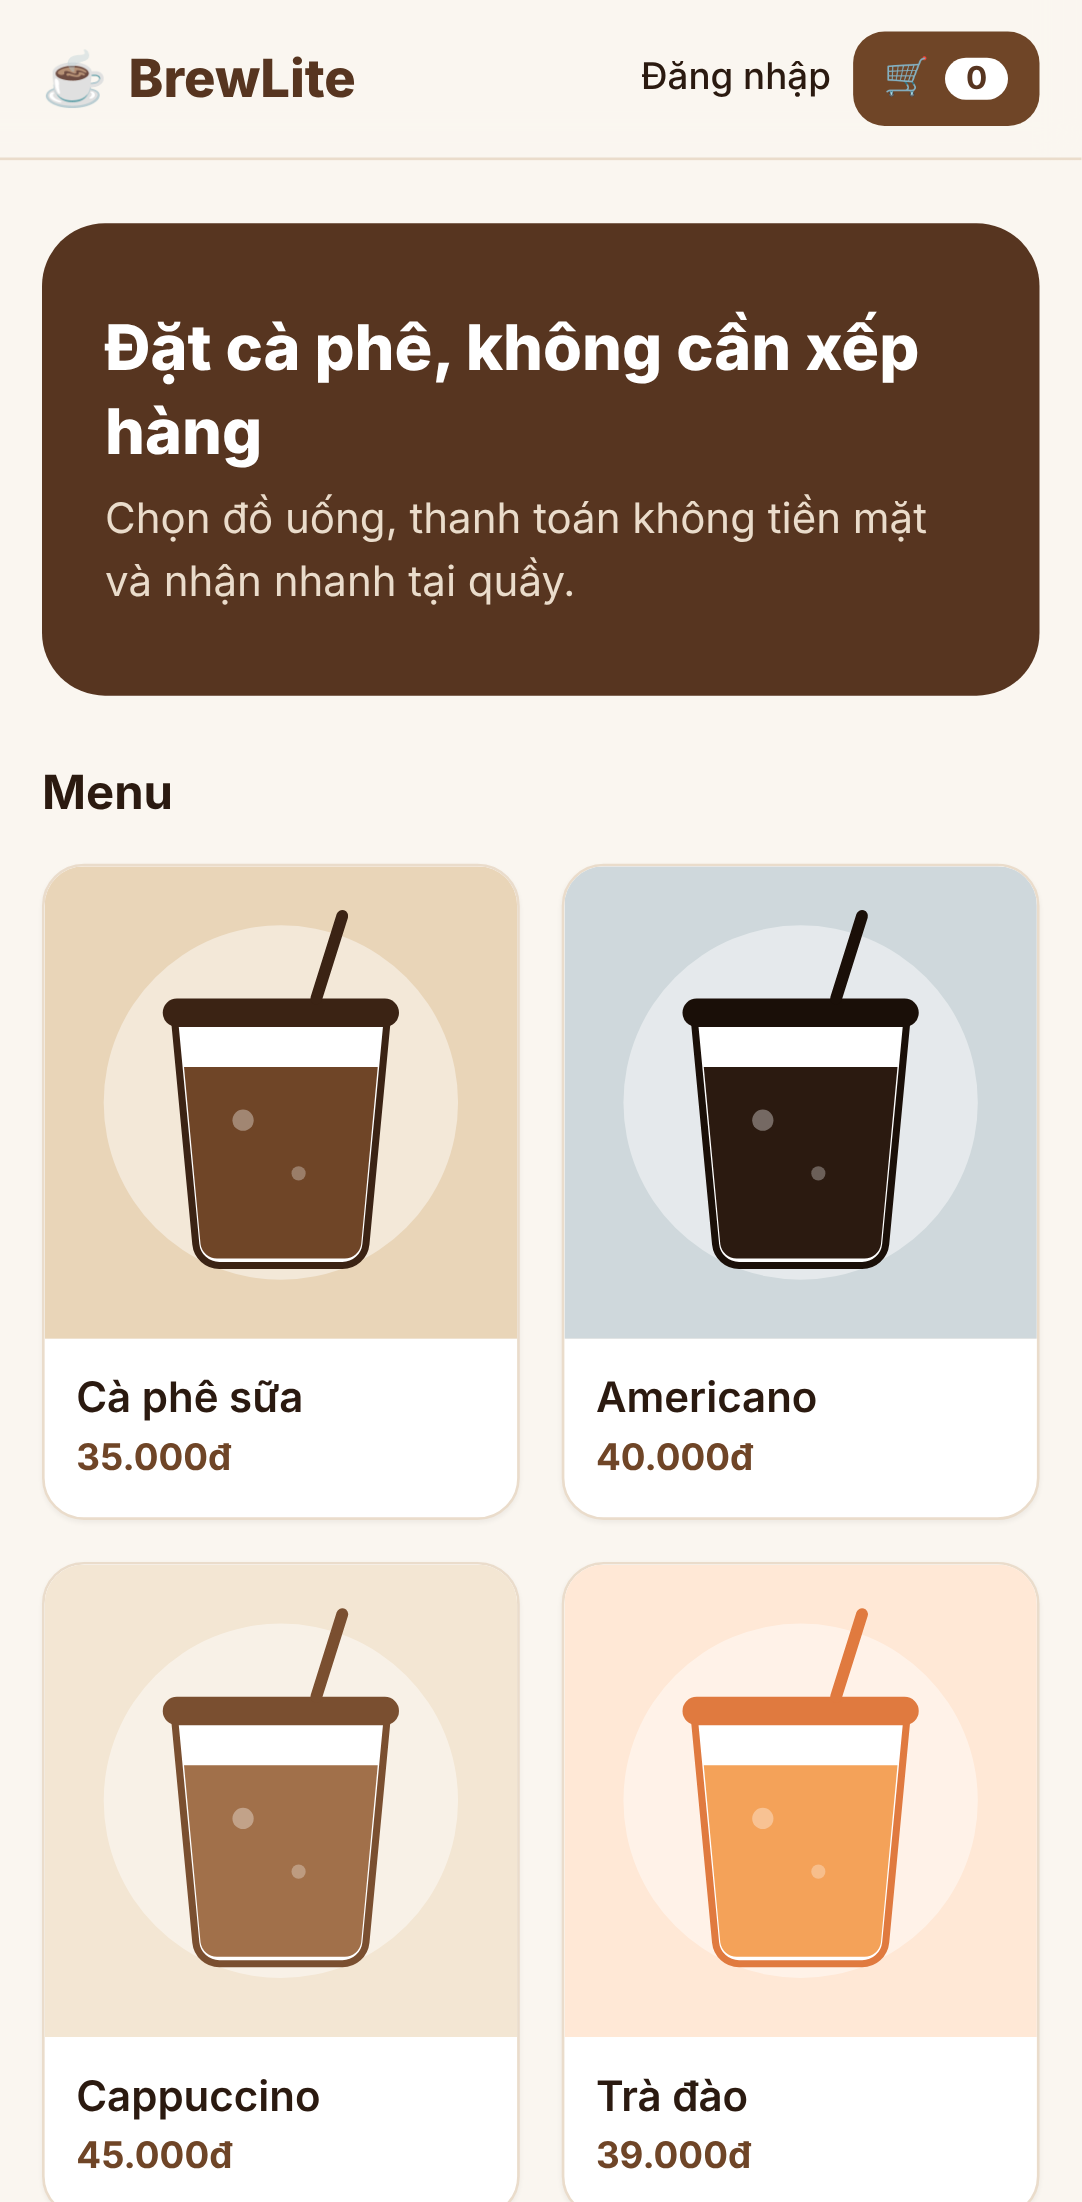
\includegraphics[width=0.62\textwidth,height=0.30\textheight,keepaspectratio]{img/shots/menu.png}}\hspace{2mm}
\end{center}\vspace{-2mm}
\qa{159}{\lvA}{Thầy: 'Em demo luồng đặt hàng từ đầu đến cuối.'}{Mở web trên điện thoại hoặc DevTools khung mobile $\rightarrow$ Menu $\rightarrow$ chọn Cappuccino, size L, Trân châu (giá 57.000đ) $\rightarrow$ Thêm vào giỏ $\rightarrow$ Giỏ hàng $\rightarrow$ Thanh toán $\rightarrow$ đăng nhập $\rightarrow$ chọn Ví điện tử, nhập BREW10 $\rightarrow$ Xác nhận $\rightarrow$ màn hình 'Đã thanh toán' có mã đơn $\rightarrow$ Lịch sử đơn. Chỉ /health để thấy version và db up.}
\qa{160}{\lvA}{Thầy: 'Chưa đăng nhập bấm thanh toán thì sao?'}{Đăng xuất, thêm món, bấm Thanh toán $\rightarrow$ bị chuyển /login?next=/checkout; đăng nhập xong quay lại /checkout, giỏ giữ nguyên.}
\qa{161}{\lvA}{Thầy: 'Thanh toán thất bại thì sao?'}{Ở trang thanh toán bật ô 'Mô phỏng thanh toán lỗi' $\rightarrow$ Xác nhận $\rightarrow$ báo thất bại, đơn PAYMENT\_FAILED, giỏ còn nguyên. Tắt ô, bấm thử lại $\rightarrow$ đơn PAID, vẫn là cùng mã đơn (không tạo đơn mới).}
\qa{162}{\lvB}{Thầy: 'Bấm thanh toán nhiều lần có bị trừ tiền hai lần không?'}{Chạy integration test INT-T16 hoặc gọi API bằng scripts/demo-api.ps1/Postman: gửi hai lần POST /payments cùng Idempotency-Key $\rightarrow$ lần 1 trả 201, lần 2 trả 200 với header Idempotent-Replayed: true; trong bảng payments chỉ có 1 dòng.}
\qa{163}{\lvB}{Thầy: 'Chứng minh không bán vượt tồn kho.'}{Chạy npm run test:integration và chỉ INT-T18 (12 khách tranh 5 ly $\rightarrow$ đúng 5 đơn, kho 0). Hoặc mở hai tab cùng mua món chỉ còn 1 ly: tab sau nhận 'không đủ hàng'.}
\qa{164}{\lvA}{Thầy: 'Áp mã WELCOME20 cho đơn 90.000đ được không?'}{Không. Đơn tối thiểu 100.000đ nên báo lỗi 'Đơn tối thiểu ...'. Thêm món cho đủ 100.000đ thì áp được, giảm 20\% tối đa 50.000đ.}
\qa{165}{\lvB}{Thầy: 'Hủy đơn đã thanh toán thì điểm ra sao?'}{Vào chi tiết đơn PAID $\rightarrow$ Hủy đơn $\rightarrow$ trạng thái CANCELLED, kho được trả; gọi GET /loyalty/me thấy số dư giảm và có dòng REVOKE (INT-T26).}
\qa{166}{\lvB}{Thầy: 'Nhân viên cập nhật trạng thái đơn thế nào?'}{Đăng nhập staff@brewlite.local, gọi PATCH /orders/:id/status với status PREPARING $\rightarrow$ READY $\rightarrow$ COMPLETED (Postman hoặc demo-api.ps1). Khách tải lại chi tiết đơn thấy trạng thái đổi. Thử nhảy cóc PENDING $\rightarrow$ COMPLETED nhận 409.}
\qa{167}{\lvA}{Thầy: 'Tắt backend thì giao diện thế nào?'}{Dừng API $\rightarrow$ trang Menu hiện 'Không kết nối được máy chủ' và nút Thử lại; bật lại API, bấm Thử lại thì menu hiện ra.}
\qa{168}{\lvA}{Thầy: 'Cài app lên điện thoại được không?'}{Mở URL production trên Chrome Android $\rightarrow$ menu $\vdots$ $\rightarrow$ Cài đặt ứng dụng / Thêm vào màn hình chính (Safari iOS: Chia sẻ $\rightarrow$ Thêm vào MH chính). Mở ra chạy toàn màn hình. Mất mạng khi mở trang mới thấy trang ngoại tuyến.}
\qa{169}{\lvA}{Thầy: 'Cho xem pipeline CI/CD.'}{Mở GitHub $\rightarrow$ Actions: lần chạy CI trên PR (các job xanh), PR demo/ci-fail bị đỏ ở bước Lint và nút Merge bị khóa; lần chạy CD trên main với Summary 'Production đang chạy \textless{}SHA\textgreater{}'; lần rollback. Mở /health để đối chiếu SHA.}
\qa{170}{\lvC}{Thầy: 'Sửa một dòng code rồi triển khai lại.'}{Tạo nhánh feat/..., sửa (ví dụ đổi chữ trên trang), commit theo Conventional Commits, mở PR $\rightarrow$ CI chạy $\rightarrow$ merge $\rightarrow$ CD build image SHA mới, deploy, smoke test $\rightarrow$ /health hiển thị SHA mới.}
\qa{171}{\lvA}{Thầy: 'Chạy hệ thống trên máy em.'}{docker compose up --build $\rightarrow$ web localhost:3000, API localhost:3001/health. Tài khoản nhân viên staff@brewlite.local / staff123 (local).}
\qa{172}{\lvB}{Thầy: 'Cho xem dữ liệu trong CSDL sau khi đặt đơn.'}{psql hoặc pgAdmin: SELECT status, total FROM orders ORDER BY id DESC LIMIT 1; SELECT * FROM payments WHERE "orderId" = ...; SELECT stock, version FROM products WHERE id = ...; SELECT * FROM loyalty\_transactions.}
\section{Câu hỏi mở rộng và câu hỏi khó}
\noindent\textit{Câu hỏi 'tại sao', 'nếu... thì sao' và hướng phát triển.} \hfill \small(11 câu)\normalsize\par\medskip
\qa{173}{\lvA}{Hạn chế lớn nhất của sản phẩm là gì?}{Cổng thanh toán mô phỏng, chưa hoàn tiền khi hủy đơn đã thanh toán; đơn PENDING chưa tự hết hạn nên có thể giữ kho mãi; chưa có giao diện nhân viên; JWT trong localStorage; gói miễn phí Render ngủ và Postgres hết hạn 30 ngày; E2E chỉ chạy Chromium, chưa kiểm thử tải.}
\qa{174}{\lvB}{Nếu có thêm thời gian, em cải tiến gì trước?}{Đơn PENDING hết hạn sau 15 phút và nhả kho (cron/job); giao diện barista có hàng đợi và thông báo thời gian thực (WebSocket/Web Push) khi READY; cổng thật + webhook + hoàn tiền; cookie HttpOnly + refresh token; rate limit /auth.}
\qa{175}{\lvC}{Nếu có 10.000 người dùng đồng thời thì sao?}{Scale ngang API (nhiều instance, stateless nhờ JWT), connection pool và chỉ mục CSDL, cache menu (CDN/Redis), chuyển migration sang job pre-deploy để tránh nhiều instance cùng chạy, tách hàng đợi cho thông báo; kiểm thử tải bằng k6 trước.}
\qa{176}{\lvC}{Vì sao không dùng Redis để khóa tồn kho?}{PostgreSQL đã có transaction, khóa dòng và optimistic lock đủ cho quy mô này; thêm Redis là thêm một thành phần phải vận hành và một nguồn sự thật thứ hai dễ lệch dữ liệu.}
\qa{177}{\lvC}{Đổi từ coupons sang promotions có làm hỏng dữ liệu cũ không?}{A2 dùng migration InitialSchema tạo bảng promotions từ đầu; CSDL tạo bởi A1 (synchronize) cần tạo lại một lần (docker compose down -v). Ở production thật sẽ viết migration đổi tên bảng (ALTER TABLE ... RENAME) để giữ dữ liệu.}
\qa{178}{\lvB}{Monorepo có nhược điểm gì?}{CI chạy cả hai app mỗi PR; repo lớn dần; quyền truy cập không tách theo app. Khắc phục: lọc job theo đường dẫn thay đổi, cache npm.}
\qa{179}{\lvC}{Nếu migration mới xóa một cột mà rollback image về bản cũ đang dùng cột đó?}{Bản cũ sẽ lỗi. Vì vậy quy tắc expand/contract: bản N thêm cột mới và ngừng dùng cột cũ; bản N+1 (sau khi chắc chắn không rollback) mới xóa cột cũ.}
\qa{180}{\lvB}{Tại sao không dùng Vercel cho Next.js?}{Vercel tốt cho Next.js nhưng sẽ chia hệ thống ra hai nền tảng (web ở Vercel, API + DB ở nơi khác), thêm cấu hình và secret. Render chạy được cả ba thành phần bằng Docker image, cùng một cơ chế deploy hook và rollback.}
\qa{181}{\lvA}{Làm sao biết code đang chạy trên production là phiên bản nào?}{Gọi /health của API và web, trường version là commit SHA; đối chiếu với lịch sử git và image trên GHCR.}
\qa{182}{\lvB}{Đồ án có áp dụng nguyên lý SOLID nào không?}{Single responsibility: controller chỉ nhận request, service xử lý nghiệp vụ, StockService chỉ lo tồn kho. Dependency inversion: PaymentsService phụ thuộc interface charge() của gateway, inject qua DI của NestJS, nên thay MockPaymentGateway bằng cổng thật không phải sửa nghiệp vụ. Open/closed: thêm mã giảm giá mới chỉ thêm dữ liệu vào bảng promotions.}
\qa{183}{\lvB}{Dependency Injection trong NestJS là gì?}{Container của NestJS tạo và cung cấp các provider (service) cho class cần dùng qua constructor, thay vì class tự new. Giúp dễ thay thế (mock trong test, đổi gateway) và giảm phụ thuộc cứng.}
\clearpage\part{Bài tập thực hành}\setcounter{section}{0}
\noindent Làm trực tiếp vào chỗ trống (in ra hoặc ghi chú trên PDF). Đáp án ở Phần III, chỉ xem sau khi đã làm xong.\par\medskip
\section{Tính tiền như server}
\noindent\textit{Dùng bảng giá: Cà phê sữa 35.000, Americano 40.000, Cappuccino 45.000, Trà đào 39.000, Latte 45.000, Bạc xỉu 38.000 (giá size M). Size S $-$5.000, L +7.000. Topping: Trân châu 5.000, Kem 7.000, Thạch dừa 5.000, Espresso shot 10.000 (mỗi loại tính một lần). BREW10: 10\%, tối đa 20.000. WELCOME20: 20\%, đơn từ 100.000, tối đa 50.000. Giảm và điểm làm tròn xuống, 1 điểm mỗi 10.000đ tổng thanh toán. Mỗi câu ghi: đơn giá từng dòng, tạm tính, giảm giá, tổng, điểm.}\par\medskip
\exq{1.1}{2 $\times$ Cà phê sữa size M, không topping, không mã.}
\writelines{3}
\exq{1.2}{1 $\times$ Latte size L + Kem + Espresso shot, mã BREW10.}
\writelines{3}
\exq{1.3}{3 $\times$ Cappuccino size S + Trân châu, mã WELCOME20.}
\writelines{3}
\exq{1.4}{2 $\times$ Trà đào size L + Thạch dừa + Trân châu, và 1 $\times$ Americano size M, mã WELCOME20.}
\writelines{4}
\exq{1.5}{2 $\times$ Bạc xỉu size M + Kem, mã WELCOME20. Hệ thống trả gì?}
\writelines{3}
\exq{1.6}{4 $\times$ Latte size L + Espresso shot, và 3 $\times$ Cappuccino size L + Kem + Trân châu, mã BREW10.}
\writelines{4}
\exq{1.7}{Client gửi toppings ['SHOT', 'SHOT'] cho 1 Latte size L. Đơn giá bao nhiêu? Vì sao?}
\writelines{3}
\exq{1.8}{Đơn 86.400đ đã PAID rồi bị hủy. Điểm thay đổi thế nào và có bản ghi gì?}
\writelines{3}
\section{State machine đơn hàng}
\noindent\textit{Điền vào bảng: \checkmark{} nếu chuyển trực tiếp từ trạng thái ở dòng sang trạng thái ở cột là hợp lệ, để trống nếu không.}\par\medskip
\exq{2.1}{Bảng 7 $\times$ 7 các chuyển tiếp.}
\begin{center}\renewcommand{\arraystretch}{1.6}\begin{tabular}{|l|c|c|c|c|c|c|c|}\hline
\diagbox[width=2.9cm]{\scriptsize Từ}{\scriptsize Tới} & \rotatebox{90}{\scriptsize PENDING} & \rotatebox{90}{\scriptsize PAID} & \rotatebox{90}{\scriptsize PREPARING} & \rotatebox{90}{\scriptsize READY} & \rotatebox{90}{\scriptsize COMPLETED} & \rotatebox{90}{\scriptsize PAYMENT\_FAILED} & \rotatebox{90}{\scriptsize CANCELLED} \\ \hline
\scriptsize PENDING & \hspace{6mm} & \hspace{6mm} & \hspace{6mm} & \hspace{6mm} & \hspace{6mm} & \hspace{6mm} & \hspace{6mm} \\ \hline
\scriptsize PAID & \hspace{6mm} & \hspace{6mm} & \hspace{6mm} & \hspace{6mm} & \hspace{6mm} & \hspace{6mm} & \hspace{6mm} \\ \hline
\scriptsize PREPARING & \hspace{6mm} & \hspace{6mm} & \hspace{6mm} & \hspace{6mm} & \hspace{6mm} & \hspace{6mm} & \hspace{6mm} \\ \hline
\scriptsize READY & \hspace{6mm} & \hspace{6mm} & \hspace{6mm} & \hspace{6mm} & \hspace{6mm} & \hspace{6mm} & \hspace{6mm} \\ \hline
\scriptsize COMPLETED & \hspace{6mm} & \hspace{6mm} & \hspace{6mm} & \hspace{6mm} & \hspace{6mm} & \hspace{6mm} & \hspace{6mm} \\ \hline
\scriptsize PAYMENT\_FAILED & \hspace{6mm} & \hspace{6mm} & \hspace{6mm} & \hspace{6mm} & \hspace{6mm} & \hspace{6mm} & \hspace{6mm} \\ \hline
\scriptsize CANCELLED & \hspace{6mm} & \hspace{6mm} & \hspace{6mm} & \hspace{6mm} & \hspace{6mm} & \hspace{6mm} & \hspace{6mm} \\ \hline
\end{tabular}\end{center}
\exq{2.2}{Khách gọi hủy đơn đang PREPARING. API trả gì? Vì sao?}
\writelines{2}
\exq{2.3}{Nhân viên gửi PATCH status = PAID cho đơn PENDING. Kết quả?}
\writelines{2}
\exq{2.4}{Hai nhân viên cùng lúc chuyển đơn PAID $\rightarrow$ PREPARING. Có bao nhiêu request thành công? Cơ chế nào?}
\writelines{3}
\exq{2.5}{Vẽ state machine đơn hàng (đủ trạng thái đầu, kết thúc, nhãn sự kiện).}
\drawgrid{9}
\section{Yêu cầu, user story và MoSCoW}
\noindent\textit{Phân loại và viết yêu cầu.}\par\medskip
\exq{3.1}{Phân loại FR hay NFR và nhóm: (a) Khách xem lịch sử đơn của mình; (b) API trả lời dưới 500 ms; (c) Mật khẩu băm bcrypt; (d) Khách nhập mã giảm giá; (e) Chạy toàn bộ hệ thống bằng một lệnh docker compose; (f) Mọi màn hình có trạng thái loading/lỗi.}
\writelines{4}
\exq{3.2}{Gán MoSCoW cho: thanh toán Ví/Thẻ; PWA; giao diện nhân viên; điểm thưởng; xem menu; thông báo khi đơn READY.}
\writelines{3}
\exq{3.3}{Viết user story và 3 tiêu chí chấp nhận dạng Given/When/Then cho chức năng 'hủy đơn'.}
\writelines{6}
\exq{3.4}{Sửa tiêu chí chấp nhận kém sau thành tiêu chí kiểm chứng được: 'Đăng nhập phải an toàn.'}
\writelines{3}
\exq{3.5}{Phân biệt: 'khách có smartphone', 'bắt buộc dùng PostgreSQL', 'khách bấm thanh toán hai lần', 'giao hàng tận nơi'. Mỗi cái là giả định, ràng buộc, rủi ro hay out-of-scope?}
\writelines{3}
\section{Use case, DFD và activity}
\exq{4.1}{Chọn include hay extend và chiều mũi tên: (1) Đặt đơn – Đăng nhập; (2) Áp mã giảm giá – Đặt đơn; (3) Thử lại thanh toán – Thanh toán; (4) Xem chi tiết – Xem menu; (5) Tích điểm – Thanh toán.}
\writelines{4}
\exq{4.2}{Vẽ use case cho actor Nhân viên quầy (đăng nhập, xem đơn, cập nhật trạng thái pha chế) trong ranh giới hệ thống.}
\drawgrid{6}
\exq{4.3}{Luồng nào sai luật DFD? (a) Khách hàng $\rightarrow$ 3.0 Tạo đơn; (b) Khách hàng $\rightarrow$ D3 orders; (c) 4.0 Thanh toán $\rightarrow$ D4 payments; (d) D2 products $\rightarrow$ D3 orders; (e) Cổng thanh toán $\rightarrow$ Nhân viên; (f) 3.0 Tạo đơn $\rightarrow$ D2 products (trừ kho).}
\writelines{3}
\exq{4.4}{Tiến trình 6.0 Truy vấn lịch sử nhận yêu cầu từ khách nhưng không có luồng ra. Lỗi gì? Sửa thế nào?}
\writelines{2}
\exq{4.5}{Vẽ activity diagram 'Khách hủy đơn' có swimlane Khách hàng / Next.js UI / NestJS API, có nhánh không được hủy.}
\drawgrid{10}
\section{Sequence, class và ERD}
\exq{5.1}{Sắp xếp các thông điệp của luồng thanh toán thành công theo đúng thứ tự: (a) INSERT payments SUCCESS; (b) SELECT * FROM orders ... FOR UPDATE; (c) charge(amount, method); (d) Kiểm tra key đã xử lý chưa; (e) COMMIT, trả 201; (f) UPDATE orders $\rightarrow$ PAID + cộng điểm; (g) POST /payments + Idempotency-Key; (h) BEGIN.}
\writelines{2}
\exq{5.2}{Vẽ sequence diagram đăng nhập: Customer, Next.js UI, NestJS API (AuthService), Database; có nhánh sai mật khẩu.}
\drawgrid{10}
\exq{5.3}{Điền bội số: User \_\_ — \_\_ Order; Order \_\_ *-- \_\_ OrderItem; OrderItem \_\_ $\rightarrow$ \_\_ Product; Order \_\_ $\rightarrow$ \_\_ Promotion; Order \_\_ — \_\_ LoyaltyTransaction.}
\writelines{3}
\exq{5.4}{Quan hệ users – orders là 1-N. FK nằm ở bảng nào, tên cột gì? Nếu thêm danh mục sản phẩm mà một sản phẩm thuộc nhiều danh mục thì thiết kế bảng thế nào?}
\writelines{3}
\exq{5.5}{Viết câu lệnh SQL tạo bảng loyalty\_transactions với các ràng buộc như đồ án.}
\writelines{7}
\section{Đồng thời và idempotency}
\noindent\textit{Lần theo dữ liệu từng bước.}\par\medskip
\exq{6.1}{Sản phẩm X có stock = 1, version = 7. Khách A và B cùng đọc rồi cùng gửi UPDATE ... WHERE id = X AND version = 7 AND stock \textgreater{}= 1. A ghi trước. Ghi lại stock, version sau mỗi bước và kết quả HTTP của A, B.}
\writelines{5}
\exq{6.2}{Chuỗi request thanh toán cho đơn \#5: (1) key K1, cổng OK; (2) key K1 lặp lại; (3) key K2 cho đơn \#5; (4) key K1 nhưng orderId \#6. Ghi mã HTTP và trạng thái đơn sau mỗi bước.}
\writelines{5}
\exq{6.3}{Chuỗi: đơn \#9 PENDING; (1) key A, cổng từ chối; (2) key A gửi lại; (3) key B, cổng OK. Ghi kết quả.}
\writelines{4}
\exq{6.4}{Vì sao thiếu UNIQUE ở idempotencyKey thì vẫn có thể bị trừ tiền hai lần dù code đã 'kiểm tra key trước'?}
\writelines{3}
\section{Kiểm thử}
\exq{7.1}{Thiết kế test giá trị biên cho số lượng mỗi dòng (hợp lệ 1–20).}
\writelines{3}
\exq{7.2}{Thiết kế test cho WELCOME20 theo giá trị biên của đơn tối thiểu và trần giảm.}
\writelines{4}
\exq{7.3}{Viết các bước một test integration chứng minh 'gửi hai lần cùng Idempotency-Key chỉ tạo một đơn'.}
\writelines{5}
\exq{7.4}{Mỗi tình huống dùng loại test nào? (a) Hàm unitPrice; (b) POST /payments với PostgreSQL thật; (c) Màn hình Menu hiện lỗi khi API sập; (d) Đặt hàng đầy đủ trên trình duyệt di động.}
\writelines{2}
\section{CI/CD và triển khai}
\exq{8.1}{Sắp xếp pipeline CD: Smoke Test, Push Registry, Push/Tag, Deploy, Docker Image, Build, Lint và Test.}
\writelines{2}
\exq{8.2}{Smoke test báo /health vẫn trả version cũ sau 6 phút. Pipeline làm gì tiếp? Production đang chạy bản nào?}
\writelines{3}
\exq{8.3}{Đặt mỗi giá trị vào đúng chỗ (repo, GitHub Secrets, GitHub Variables, Render Environment): JWT\_SECRET, RENDER\_DEPLOY\_HOOK\_API, API\_URL, DATABASE\_URL, .env.example, CORS\_ORIGIN.}
\writelines{3}
\exq{8.4}{Migration mới bị lỗi cú pháp được merge vào main. Mô tả chuyện gì xảy ra từ lúc merge tới khi kết thúc pipeline.}
\writelines{4}
\exq{8.5}{Viết lệnh để phát hành phiên bản 2.0.0 và lệnh rollback tay về commit abc123... (SHA đầy đủ).}
\writelines{3}
\section{Ma trận truy vết}
\noindent\textit{Điền một dòng của ma trận truy vết.}\par\medskip
\exq{9.1}{Điền ma trận cho FR-11 Hủy đơn: Use-case/User Story | Thiết kế/Sơ đồ | Code/API | Test.}
\writelines{4}
\exq{9.2}{Điền ma trận cho FR-12 Điểm thưởng.}
\writelines{4}
\clearpage\part{Đáp án bài tập}
\subsection*{Tính tiền như server}
\ansq{1.1}{Đơn giá 35.000; tạm tính 70.000; giảm 0; tổng 70.000; 7 điểm.}
\ansq{1.2}{Đơn giá 45.000 + 7.000 + 7.000 + 10.000 = 69.000; tạm tính 69.000; giảm $\lfloor$6.900$\rfloor$ = 6.900; tổng 62.100; 6 điểm.}
\ansq{1.3}{Đơn giá 45.000 $-$ 5.000 + 5.000 = 45.000; tạm tính 135.000 ($\ge$ 100.000 nên áp được); giảm 27.000 (dưới trần 50.000); tổng 108.000; 10 điểm.}
\ansq{1.4}{Trà đào: 39.000 + 7.000 + 5.000 + 5.000 = 56.000 $\times$ 2 = 112.000; Americano 40.000; tạm tính 152.000; giảm 30.400; tổng 121.600; 12 điểm.}
\ansq{1.5}{Đơn giá 45.000; tạm tính 90.000 \textless{} 100.000 nên mã bị từ chối: 400 'Đơn tối thiểu 100000đ để dùng mã WELCOME20'. Đơn không được tạo; khách bỏ mã hoặc thêm món.}
\ansq{1.6}{Latte 62.000 $\times$ 4 = 248.000; Cappuccino 45.000 + 7.000 + 7.000 + 5.000 = 64.000 $\times$ 3 = 192.000; tạm tính 440.000; 10\% = 44.000 nhưng trần 20.000 $\rightarrow$ giảm 20.000; tổng 420.000; 42 điểm.}
\ansq{1.7}{45.000 + 7.000 + 10.000 = 62.000. Server bỏ trùng topping (mỗi loại tính một lần), không cộng 20.000.}
\ansq{1.8}{Khi PAID cộng $\lfloor$86.400/10.000$\rfloor$ = 8 điểm và ghi LoyaltyTransaction EARN 8. Khi hủy thu hồi 8 điểm, ghi REVOKE 8; số dư quay về như trước.}
\subsection*{State machine đơn hàng}
\ansq{2.1}{Hợp lệ đúng 9 ô: PENDING $\rightarrow$ PAID, PAYMENT\_FAILED, CANCELLED; PAYMENT\_FAILED $\rightarrow$ PENDING, CANCELLED; PAID $\rightarrow$ PREPARING, CANCELLED; PREPARING $\rightarrow$ READY; READY $\rightarrow$ COMPLETED. Còn lại 40 ô trống (kể cả đường chéo).}
\begin{center}\renewcommand{\arraystretch}{1.3}\begin{tabular}{|l|c|c|c|c|c|c|c|}\hline
\diagbox[width=2.9cm]{\scriptsize Từ}{\scriptsize Tới} & \rotatebox{90}{\scriptsize PENDING} & \rotatebox{90}{\scriptsize PAID} & \rotatebox{90}{\scriptsize PREPARING} & \rotatebox{90}{\scriptsize READY} & \rotatebox{90}{\scriptsize COMPLETED} & \rotatebox{90}{\scriptsize PAYMENT\_FAILED} & \rotatebox{90}{\scriptsize CANCELLED} \\ \hline
\scriptsize PENDING &  & \textcolor{good}{\checkmark} &  &  &  & \textcolor{good}{\checkmark} & \textcolor{good}{\checkmark} \\ \hline
\scriptsize PAID &  &  & \textcolor{good}{\checkmark} &  &  &  & \textcolor{good}{\checkmark} \\ \hline
\scriptsize PREPARING &  &  &  & \textcolor{good}{\checkmark} &  &  &  \\ \hline
\scriptsize READY &  &  &  &  & \textcolor{good}{\checkmark} &  &  \\ \hline
\scriptsize COMPLETED &  &  &  &  &  &  &  \\ \hline
\scriptsize PAYMENT\_FAILED & \textcolor{good}{\checkmark} &  &  &  &  &  & \textcolor{good}{\checkmark} \\ \hline
\scriptsize CANCELLED &  &  &  &  &  &  &  \\ \hline
\end{tabular}\end{center}
\ansq{2.2}{409 INVALID\_TRANSITION vì PREPARING chỉ được chuyển sang READY; quán đã bắt đầu pha chế.}
\ansq{2.3}{400: nhân viên chỉ được đặt PREPARING, READY, COMPLETED; PAID chỉ do thanh toán thành công sinh ra.}
\ansq{2.4}{Đúng 1. UPDATE orders SET status = 'PREPARING' WHERE id = ? AND status = 'PAID': request đầu đổi được 1 dòng, request sau 0 dòng nên bị từ chối (409).}
\ansq{2.5}{Chấm đầu $\rightarrow$ PENDING. PENDING –thanh toán OK$\rightarrow$ PAID –nhân viên bắt đầu$\rightarrow$ PREPARING –pha xong$\rightarrow$ READY –khách nhận$\rightarrow$ COMPLETED $\rightarrow$ chấm kết thúc. PENDING –cổng từ chối$\rightarrow$ PAYMENT\_FAILED –thử lại$\rightarrow$ PENDING. PENDING, PAYMENT\_FAILED, PAID –khách hủy / hoàn kho$\rightarrow$ CANCELLED $\rightarrow$ chấm kết thúc.}
\subsection*{Yêu cầu, user story và MoSCoW}
\ansq{3.1}{(a) FR – lịch sử đơn (FR-09); (b) NFR – hiệu năng (NFR-01); (c) NFR – bảo mật (NFR-03); (d) FR – đặt đơn/khuyến mãi (FR-06); (e) NFR – khả năng triển khai (NFR-08); (f) NFR – tính khả dụng (NFR-06).}
\ansq{3.2}{Must: thanh toán, xem menu. Should: điểm thưởng. Could: PWA. Won't (bản 2.0): giao diện nhân viên, thông báo READY.}
\ansq{3.3}{Là khách hàng, tôi muốn hủy đơn chưa pha chế để đổi ý. (1) Given đơn PENDING của tôi, When tôi bấm Hủy, Then đơn CANCELLED và tồn kho được trả. (2) Given đơn PAID có 8 điểm đã cộng, When tôi hủy, Then điểm giảm 8 và có giao dịch REVOKE. (3) Given đơn PREPARING, When tôi hủy, Then nhận 409 và đơn không đổi.}
\ansq{3.4}{Ví dụ: sai mật khẩu trả 401 và không tiết lộ email có tồn tại hay không; mật khẩu lưu dạng băm bcrypt; gọi API cần đăng nhập không có token trả 401; token hết hạn sau 1 ngày.}
\ansq{3.5}{Giả định (A-01); ràng buộc (C-01); rủi ro (R-01); out-of-scope.}
\subsection*{Use case, DFD và activity}
\ansq{4.1}{(1) Đặt đơn include Đăng nhập (mũi tên từ Đặt đơn tới Đăng nhập). (2) Áp mã extend Đặt đơn (mũi tên từ Áp mã về Đặt đơn). (3) Thử lại extend Thanh toán. (4) Xem chi tiết extend Xem menu. (5) Tích điểm extend Thanh toán, điều kiện [đơn PAID].}
\ansq{4.2}{Actor Nhân viên ngoài hình chữ nhật 'BrewLite'; các elip UC-04 Đăng nhập, Xem đơn, UC-11 Cập nhật trạng thái pha chế; association từ actor; Cập nhật trạng thái include Đăng nhập (hoặc ghi tiền điều kiện role STAFF).}
\ansq{4.3}{Sai: (b) tác nhân nối thẳng kho; (d) kho nối thẳng kho; (e) tác nhân nối thẳng tác nhân. Đúng: (a), (c), (f).}
\ansq{4.4}{Hố đen. Thêm luồng 'danh sách đơn' từ 6.0 về Khách hàng và luồng đọc từ D3 orders vào 6.0.}
\ansq{4.5}{Bắt đầu $\rightarrow$ Khách mở chi tiết đơn $\rightarrow$ UI hiện nút Hủy nếu trạng thái thuộc PENDING/PAYMENT\_FAILED/PAID $\rightarrow$ Khách bấm Hủy $\rightarrow$ UI gửi POST /orders/:id/cancel + JWT $\rightarrow$ API kiểm tra chủ đơn [không: 403] $\rightarrow$ assertTransition [không hợp lệ: 409, UI báo lỗi] $\rightarrow$ BEGIN, UPDATE status = CANCELLED WHERE status = hiện tại, trả kho, [đã PAID] thu hồi điểm, COMMIT $\rightarrow$ UI hiện 'Đã hủy' $\rightarrow$ kết thúc.}
\subsection*{Sequence, class và ERD}
\ansq{5.1}{g $\rightarrow$ d $\rightarrow$ h $\rightarrow$ b $\rightarrow$ c $\rightarrow$ f $\rightarrow$ a $\rightarrow$ e.}
\ansq{5.2}{Customer nhập email/mật khẩu $\rightarrow$ UI POST /auth/login $\rightarrow$ API ValidationPipe [sai định dạng: 400] $\rightarrow$ SELECT user WHERE email $\rightarrow$ alt không có user hoặc bcrypt.compare sai: 401 'Sai email hoặc mật khẩu' / đúng: ký JWT (1 ngày) $\rightarrow$ 200 \{accessToken, user\} $\rightarrow$ UI lưu token (Zustand persist) $\rightarrow$ chuyển trang next hoặc /.}
\ansq{5.3}{1 — 0..*; 1 *-- 1..*; 0..* $\rightarrow$ 1; 0..* $\rightarrow$ 0..1; 1 — 0..2.}
\ansq{5.4}{FK ở orders: orders.userId $\rightarrow$ users.id. Quan hệ N-N cần bảng trung gian product\_categories(productId FK, categoryId FK, PK ghép (productId, categoryId)).}
\ansq{5.5}{CREATE TABLE loyalty\_transactions (id SERIAL PRIMARY KEY, "userId" INT NOT NULL REFERENCES users(id), "orderId" INT NOT NULL REFERENCES orders(id), type VARCHAR NOT NULL, points INT NOT NULL, "createdAt" TIMESTAMPTZ NOT NULL DEFAULT now(), UNIQUE ("orderId", type));}
\subsection*{Đồng thời và idempotency}
\ansq{6.1}{A: 1 dòng bị ảnh hưởng $\rightarrow$ stock 0, version 8 $\rightarrow$ A nhận 201. B: 0 dòng (version đã là 8) $\rightarrow$ đọc lại stock 0, version 8 $\rightarrow$ stock \textless{} 1 $\rightarrow$ ROLLBACK, B nhận 409 OUT\_OF\_STOCK. Kho không âm.}
\ansq{6.2}{(1) 201, đơn PAID. (2) 200 + Idempotent-Replayed: true, vẫn PAID, không có payment mới. (3) 409 ORDER\_NOT\_PAYABLE (đơn đã PAID). (4) 409: key K1 đã dùng cho đơn khác.}
\ansq{6.3}{(1) 402, đơn PAYMENT\_FAILED, payment FAILED lưu với key A. (2) Trả lại kết quả cũ 402 + Idempotent-Replayed, không gọi cổng. (3) Đơn PAYMENT\_FAILED $\rightarrow$ PENDING $\rightarrow$ PAID, 201, cộng điểm một lần.}
\ansq{6.4}{Hai request đồng thời cùng kiểm tra lúc chưa có bản ghi, cả hai đều thấy 'chưa có' rồi cùng xử lý (race condition kiểm tra-rồi-ghi). UNIQUE ở CSDL và khóa dòng FOR UPDATE bảo đảm chỉ một request ghi được.}
\subsection*{Kiểm thử}
\ansq{7.1}{0 $\rightarrow$ 400; 1 $\rightarrow$ hợp lệ; 20 $\rightarrow$ hợp lệ; 21 $\rightarrow$ 400. Thêm: -1, giá trị không phải số nguyên (1.5, 'abc') $\rightarrow$ 400.}
\ansq{7.2}{Tạm tính 99.999 (hoặc 99.000) $\rightarrow$ 400; 100.000 $\rightarrow$ giảm 20.000; 250.000 $\rightarrow$ giảm 50.000 (đúng bằng trần); 300.000 $\rightarrow$ giảm 50.000 (bị chặn trần).}
\ansq{7.3}{Đăng ký user, tạo sản phẩm stock 10 $\rightarrow$ gửi POST /orders với key K $\rightarrow$ 201, lưu id $\rightarrow$ gửi lại cùng key $\rightarrow$ 200 + Idempotent-Replayed, cùng id $\rightarrow$ kiểm tra COUNT(orders) của user = 1 và stock chỉ giảm một lần. Biến thể: 5 request song song bằng Promise.all.}
\ansq{7.4}{(a) Unit test; (b) Integration test; (c) Test component (Vitest + Testing Library); (d) E2E (Playwright).}
\subsection*{CI/CD và triển khai}
\ansq{8.1}{Push/Tag $\rightarrow$ Lint và Test $\rightarrow$ Build $\rightarrow$ Docker Image $\rightarrow$ Push Registry $\rightarrow$ Deploy $\rightarrow$ Smoke Test.}
\ansq{8.2}{Bước smoke test thất bại $\rightarrow$ bước Rollback chạy: gọi deploy hook với image SHA cũ (đọc từ /health trước khi deploy), smoke test lại với SHA cũ, rồi pipeline kết thúc với trạng thái lỗi. Production vẫn chạy bản cũ.}
\ansq{8.3}{JWT\_SECRET: Render Environment (Render sinh). RENDER\_DEPLOY\_HOOK\_API: GitHub Secrets (environment production). API\_URL: GitHub Variables. DATABASE\_URL: Render Environment (lấy từ DB). .env.example: repo (giá trị giả). CORS\_ORIGIN: Render Environment.}
\ansq{8.4}{CI đã chạy integration test trên schema từ migration nên thường đã đỏ và không merge được. Nếu vẫn lọt: CD build, deploy API $\rightarrow$ container mới chạy migration trong 1 transaction $\rightarrow$ lỗi $\rightarrow$ rollback transaction, process thoát $\rightarrow$ /health không bao giờ 200, Render giữ bản cũ $\rightarrow$ smoke test hết lượt thử $\rightarrow$ rollback (deploy lại SHA cũ) $\rightarrow$ pipeline đỏ. CSDL không bị thay đổi.}
\ansq{8.5}{git tag -a v2.0.0 -m 'BrewLite 2.0.0' \&\& git push origin v2.0.0. Rollback: GitHub $\rightarrow$ Actions $\rightarrow$ CD $\rightarrow$ Run workflow $\rightarrow$ rollback\_to = SHA đầy đủ (hoặc gh workflow run cd.yml -f rollback\_to=\textless{}SHA\textgreater{}).}
\subsection*{Ma trận truy vết}
\ansq{9.1}{UC-09, US-11 | Activity-01 (nhánh hủy sau thanh toán lỗi), state machine đơn hàng | POST /orders/:id/cancel – orders.service.ts | INT-T13, INT-T22, UI-E.}
\ansq{9.2}{UC-10, US-09, US-13 | Class-01 LoyaltyTransaction, Sequence-01 bước cộng điểm | awardPoints/revokePoints trong promotions.service.ts, GET /loyalty/me | UT-11, INT-T16, T21, T22, T26, T27.}
\end{document}